\def \sectionauthors {Philipp Kraft}

\subsection{Einleitung}
Das Webinterface hat auf der einen Seite die Aufgabe die Kommunikation mit der
Kennzeichenerkennung und der Fahrzeugerkennung sicherzustellen und auf der
anderen Seite die Verwaltung und Darstellung der gewonnen Daten.

\subsection{Verwendete Technologien}
\subsubsection{HTML}
\acs*{HTML} steht hierbei für \acl*{HTML} und ist eine Auszeichnungssprache
welche vom \ac*{W3C}\footnote{\url{https://www.w3.org} } entwickelt wird.
\ac*{HTML} ist De-Facto-Standard um Inhalte in Browsern darzustellen.
\acs*{HTML} ist dabei aber nicht für die visuelle Darstellung verantwortlich
sondern nur für die semantische Struktur. Der Sinn dahinter ist, dass der Inhalt
und die Vorgaben an die Darstellung möglichst gut getrennt ist. Für die
Formatierung kommt die Stylesheet-Sprache \ac*{CSS} zum Einsatz, welche
ebenfalls vom \acl*{W3C} entwickelt wird. Die aktuellste Version der \acs*{HTML}
Spezifikation ist
HTML5\footnote{\url{https://www.w3.org/2014/10/html5-rec.html.en}} und wurde am
28. Oktober 2014 vom \acs*{W3C} vorgelegt.

\begin{figure}[H]
  \centering
  
\includegraphics[width=0.2\linewidth]{webinterface/html5_logo.pdf}
  \caption{HTML5 Logo von \citeurl[]{html5logo}}
\end{figure}

\paragraph{Beispielhafte HTML Seite}\mbox{}\\
Eine \acs*{HTML} Seite setzt sich aus einer Vielzahl von sogenannten Elementen
zusammen. Ein Element besteht aus einem Start Tag und aus einem End Tag, der
Inhalt wird zwischen diese Tags geschrieben. Nun folgt eine einfache HTML Seite,
welche die Grundlegenden Funktionen von HTML und CSS darlegen soll.

\begin{listing}[H]
  \begin{minted}{html}
    <!DOCTYPE html>
    <html>
    <head>
    <title>Titel</title>ü
    </head>
    <body>

    <h1>Überschrift</h1>
    <p>Paragraph</p>

    </body>
    </html>
  \end{minted}
  \caption{index.html}
  \label{lst:simple_html_site}
\end{listing}

Das Element \verb|<!DOCTYPE html>| deklariert, dass die folgende Seite den HTML5
Standard verwendet. Danach folgt mit \verb|<html>| das Wurzelelement, dass alle
anderen Elemente beinhaltet. Das \verb|<head>| Element beinhaltet verschiedene
Metadaten d.h. Daten die nicht angezeigt werden. Im oben gezeigten Beispiel
Code~\ref{lst:simple_html_site} wird nur der Title des Dokuments gesetzt, dieser
wird im Browser Tab angezeigt. Es können aber auch noch andere Daten gesetzt
bzw. eingebunden werden:

\begin{itemize}
  \item Character Set
  \item Styles
  \item Scripts
  \item Viewport
  \item Sonstige Metainformationen (Author, Keywords)
\end{itemize}

\begin{figure}[H]
  \centering
  \frame{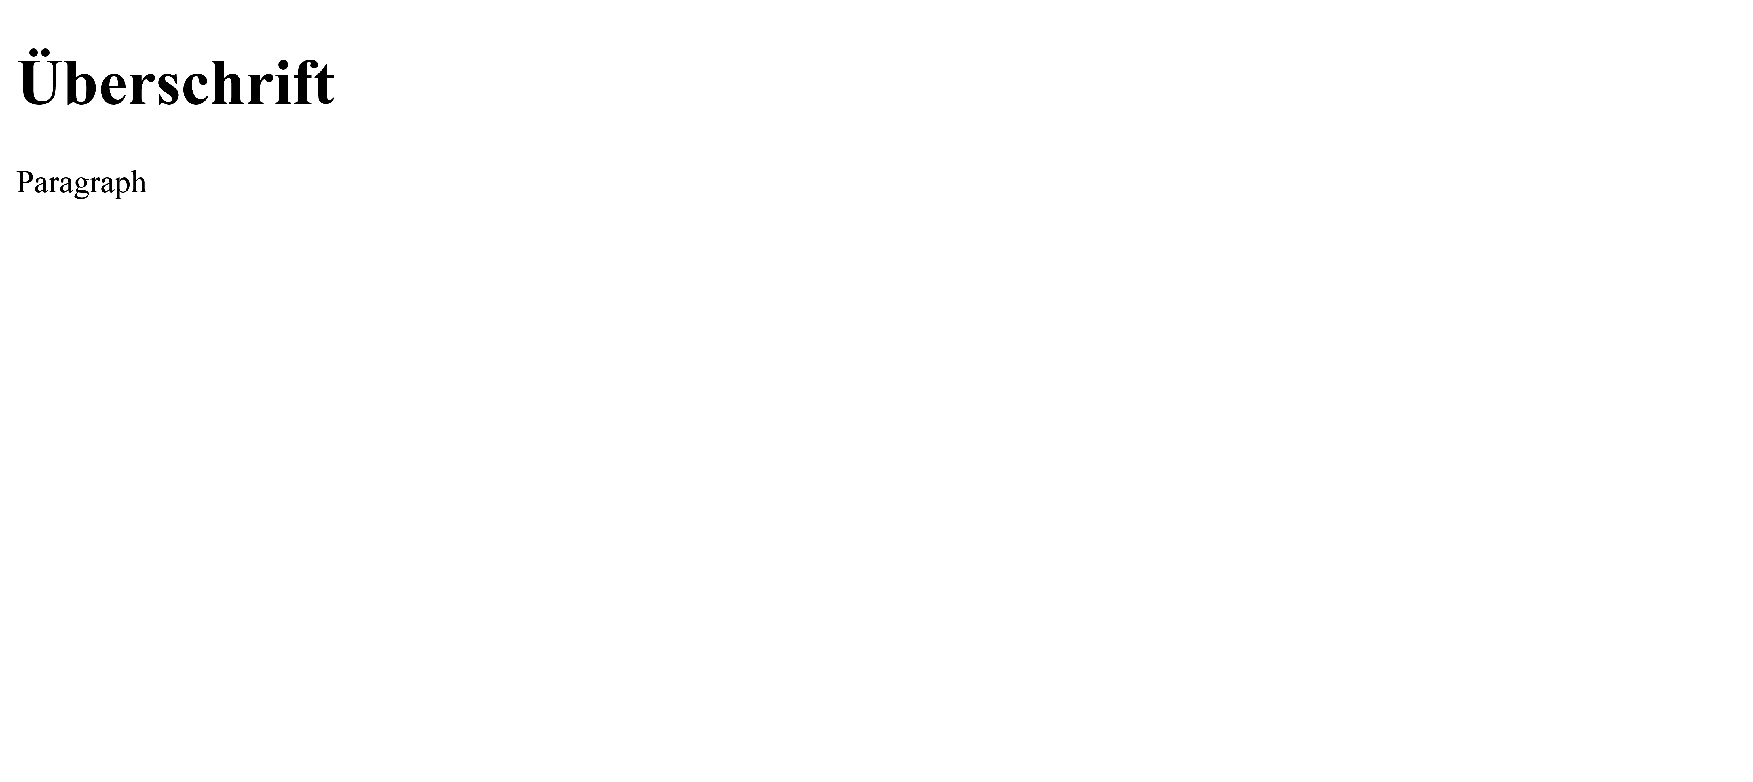
\includegraphics[width=1\linewidth]{webinterface/simple_html_site.pdf}}
  \caption{Einfache HTML Seite von \citeurl[]{html5logo}}
\end{figure}

\subsubsection{CSS}
Wie bereits angesprochen ist \ac*{CSS} für die Formatierung bzw. die visuelle
Darstellung der einzelnen HTML-Elemente verantwortlich. Der Standard wird wie
bei HTML vom \acs*{W3C} spezifiziert und die aktuellste Version ist CSS3 was so
viel bedeutet wie \acs*{CSS} Level 3, wobei nur einzelne Teile als Empfehlung
durch das \acs*{W3C} vorgelegt wurden, beispielweise das CSS Color Module Level
3\footnote{\url{https://www.w3.org/TR/css-color-3}}. Um die Funktion
darzustellen wird die vorherige HTML Seite nun mit CSS ergänzt.

\begin{listing}[H]
  \begin{minted}{css}
    body {
      background-color: deepskyblue;
    }

    h1 {
      color: white;
      text-align: center;
      font-family: verdana;
    }

    p {
      color: wheat;
      font-family: verdana;
      font-size: 20px;
    }
  \end{minted}
  \caption{style.css}
\end{listing}

Nun muss dieses Stylesheet nur noch im \verb|<head>| Tag mit\\
\mintinline{css}{  <link rel="stylesheet" href="style.css">} eingebunden werden.

\begin{figure}[H]
  \centering
  \frame{
\includegraphics[width=1\linewidth]{webinterface/simple_html_site_with_css.pdf}}
  \caption{Einfache HTML Seite mit CSS}
\end{figure}

Es lässt sich nun erkennen, dass sich die Webseite deutlich verändert hat. Dabei
bieten HTML und CSS bieten noch viel mehr Funktionen, eine ausführliche
Dokumentation der Funktionen sind auf der Website
w3schools\footnote{\url{https://www.w3schools.com/html} und
\url{https://www.w3schools.com/css}} zu finden.

\subsubsection{JavaScript}
Es folgt nun eine weitere sehr wichtige Technologie und die meist verwendete
Programmiersprache überhaupt laut der Stack Overflow Developer Survey
2020\footnote{\url{https://insights.stackoverflow.com/survey/2020}}. \ac*{JS}
ermöglicht es dynamische Webseiten zu erstellen, dabei wird der Code direkt
lokal im Browser ausgeführt. Jedoch ist JavaScript nicht mehr nur auf das
Frontend\footnote{Präsentationsebene in Form der grafischen Benutzeroberfläche}
mehr beschränkt, es möglich mit Frameworks wie Node.js auch
Backend\footnote{Verarbeitung von Daten auf beispielsweise einem Server}
Applikationen zu schreiben und somit ist es möglich Full-Stack\footnote{Front-
und Backend}-Anwendungen vollständig mit \acl*{JS} zu entwickeln. Eine der
wichtigsten Anwendungsgebiete ist die Manipulation von Elementen über das
\ac*{DOM}. Der Standards wird unter dem Namen ECMA Script von der Organisation
Ecma International\footnote{\url{https://www.ecma-international.org}}
veröffentlicht und die aktuellste Version ist \textbf{ECMA-262}.

\subsubsection{PHP}
\ac*{PHP} ist eine Skriptsprache um dynamische Webseiten zu realisieren, jedoch
wird nicht wie bei \acl*{JS} der Code auf dem Client ausgeführt sondern auf dem
Server, dort wird die HTML-Ausgabe generiert und dem Client zugesendet. Somit
ist es nicht möglich den Code als Benutzer zu betrachten. Grundsätzlich ist PHP
als synchrone Sprache geplant worden, es ist jedoch auch möglich asynchron zu
Programmieren um die Performance zu steigern. Die aktuellste Version ist
\acs*{PHP} 8\footnote{\url{https://www.php.net/docs.php}}.


\subsubsection{TailwindCSS}
Es gibt eine Vielzahl von CSS-Frameworks, das Ziel ist ein einfacheres und
schnelleres erstellen von Webseiten, dazu gehören neben TailwindCSS folgende
relevanten Frameworks.

\begin{itemize}
  \item Bootstrap (\url{https://getbootstrap.com})
  \item Foundation (\url{https://get.foundation})
  \item Materialize (\url{https://materializecss.com})
\end{itemize}

Viele von diesen CSS Frameworks verwenden vorgefertigte Components welche direkt
verwendet werden können, dies führt dazu, dass die Entwicklung sehr rasch ist.
Dort unterscheidet sich TailwindCSS von den anderen CSS Frameworks, dort
existieren sogenannte Utility-Classes, diese können direkt im \acs*{HTML} auf
die einzelnen Elemente angewendet werden.

%\subsubsection{Vue}

\subsubsection{Laravel}
Laravel\footnote{\url{https://laravel.com/}} ist ein Open-Source PHP-Framework,
es erleichtert die Entwicklung und erhöht die Sicherheit und auch durch die
zahlreichen First-Party-Packages bietet Laravel ein sehr hochwertiges Ecosystem.
Da Laravel ein sehr wichtiger Bestandteil des Webinterfaces ist wird später noch
genauer auf die einzelne Funktionen des Frameworks eingegangen. Laravel wird
seit Juni 2011 entwickelt und erhält jährlich eine neue Version, aktuell ist
Laravel 8 die neuste Version.\\

Das Framework folgt dem sogenannten \ac*{MVC} Muster das bedeutet, dass die
Programmierlogik in drei verschiedene Teile unterteilt wird. Der Sinn dahinter
ist, dass die Anwendung dadurch sehr flexibel ist und später leichter erweitert
werden kann oder einzelne Teile wiederverwendet werden können.

\begin{itemize}
  \item \textbf{Model} \\
  Hier befindet sich die Datenstruktur der Anwendung. In Laravel kann dies
  beispielsweise das Model \verb|User| sein.
  \item \textbf{View} \\
  In der View befindet sich die Präsentationsebene, im Fall von Laravel sind das
  Components und Layouts.
  \item \textbf{Controller} \\
  In den Controllern der Anwendung befindet sich die Logik um beispielsweise
  durch das Absenden eines Formulares einen Eintrag in der Datenbank zu
  erstellen. 
\end{itemize}

Ein Anfrage auf eine Webseite läuft in 6. Schritten ab:

\begin{itemize}
  \item \textbf{1. Schritt:} Der Benutzer führt eine HTTP-Anfragemethode aus
  \item \textbf{2. Schritt:} Die Anfrage wird geroutet
  \item \textbf{3. Schritt:} Der Controller interagiert mit dem Model
  \item \textbf{4. Schritt:} Das Model greift auf die Datenbank zu
  \item \textbf{5. Schritt:} Der Controller liefert die Daten an eine View
  \item \textbf{6. Schritt:} View mit den Daten werden an den Client gesendet
\end{itemize}

\begin{figure}[H]
  \centering
  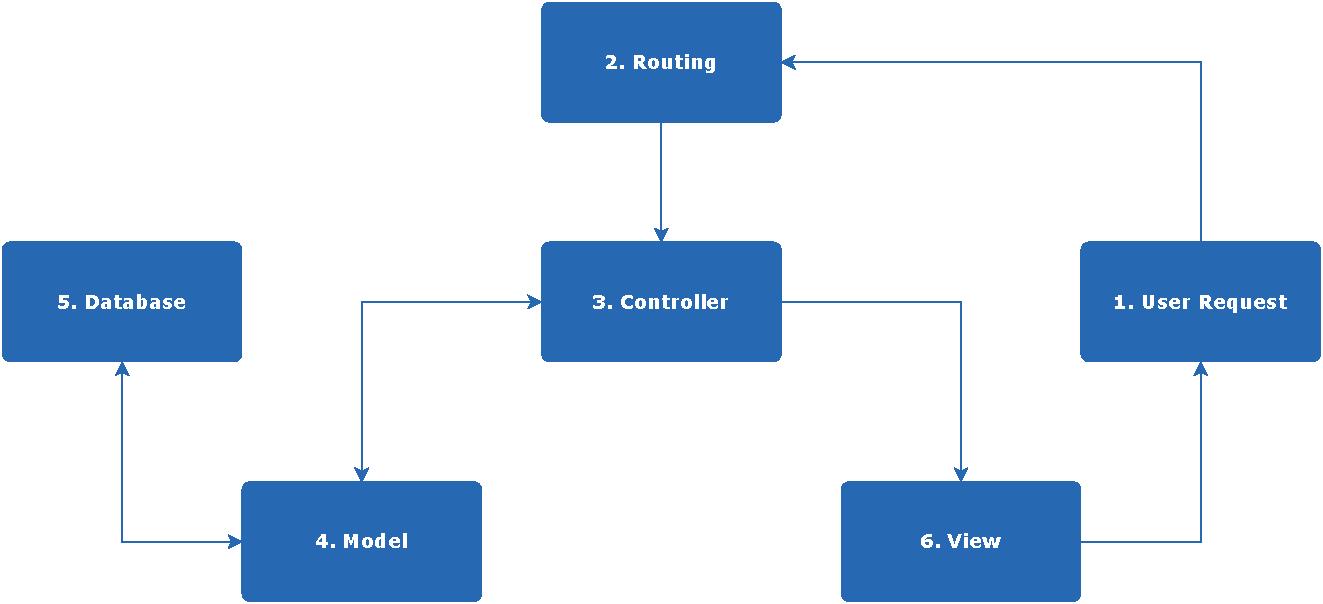
\includegraphics[width=1\linewidth]{webinterface/mvc_laravel.pdf}
  \caption{Laravel MVC Muster}
\end{figure}

\paragraph{Routing}\mbox{}\\
In Laravel erfolgt durch ein Routefile unter \verb|routes/web.php|. API Requests
haben ein eigenes Routefile unter \verb|routes/api.php| und erhalten einen
\verb|/api| Prefix. Diese Dateien werden dann automatisch durch einen Service
Provider von Laravel geladen.\\

Der Laravel Router erlaubt folgende HTTP-Anfragemethoden:
\begin{itemize}
  \item \textbf{GET} (Fordert Ressource an)\\
  \mintinline{php}{  Route::get($uri, $callback);}
  \item \textbf{POST} (Neue Ressource erstellen)\\
  \mintinline{php}{  Route::post($uri, $callback););}
  \item \textbf{PUT} (Ressource ersetzen oder erstellen)\\
  \mintinline{php}{  Route::put($uri, $callback);}
  \item \textbf{PATCH} (Ressource ändern)\\
  \mintinline{php}{  Route::patch($uri, $callback);}
  \item \textbf{DELETE} (Löscht Ressource)\\
  \mintinline{php}{  Route::delete($uri, $callback);}
  \item \textbf{OPTIONS} (Liste von unterstützen Methoden des Servers)\\
  \mintinline{php}{  Route::options($uri, $callback);}
\end{itemize}

Im folgenden Ausschnitt Code~\ref{lst:user_routes} werden ein Teil der Routen
von den Benutzern dargelegt. Dabei lässt sich erkennen, dass die Routen sich in
einer Gruppe befinden, welche den Prefix \verb|/admin| und die Middleware
\verb|verified| hat das bedeutet, dass der Benutzer eingeloggt sein muss um
diese Routen aufzurufen. Dabei verweisen die Routen auf einzelne Methoden im
UserController. Schlussendlich werden mit der name-Methode die Routen benannt,
damit sie später im Code einfach referenziert werden können.

\begin{listing}[H]
  \begin{minted}{php}
    <?php
    Route::group(['middleware' => 'verified', 'prefix' => 'admin'], 
    function () {
      Route::get('users', [UserController::class, 'index'])->name('users.index');
      Route::get('users/create', [UserController::class, 'create'])->name('users.create');
      Route::post('users', [UserController::class, 'store'])->name('users.store');
    });
  \end{minted}
  \caption{web.php}
  \label{lst:user_routes}
\end{listing}

\paragraph{Blade Templates}\mbox{}\\
Blade ist eine Template Engine, die mit Laravel mitgeliefert wird. Blade
erleichtert und vereinfacht das Verwenden von PHP Code in HTML, dabei wird der
Blade Syntax in normalen PHP Code compiliert. Blade Dateien werden mit der
Extension \verb|.blade.php| erstellt. Damit der Inhalt der einzelnen Seiten
dynamisch ist müssen Daten übergeben werden, dies erfolgt über die Controller.\\

Um nun Inhalt innerhalb eines Blade Files anzuzeigen verwendet Blade doppelt
Geschweifte Klammern.

\begin{listing}[H]
  \begin{minted}{php}
    Hallo, {{ $user->full_name }}.
  \end{minted}
  \caption{example.blade.php}
  \label{lst:blade_example}
\end{listing}

Im Code~\ref{lst:blade_example} wird nun auf das übergebene Model \verb|User|
zugegriffen und der Name ausgegeben.

\paragraph{Controllers}\mbox{}\\
Es besteht theoretisch die Möglichkeit die komplette Logik für die bearbeitung
von Anfragen direkt in den Route Files zu platzieren, dies ist jedoch sehr
unübersichtlich und deshalb ist es sinnvoll diese Logik in Controller Klassen
auszulagern. Dabei werden ähnliche Anfragen zusammengeführt, so ist es sinnvoll
alle Anfragen wie in Code~\ref{lst:user_routes} im gleichen Controller
zusammenzuführen.

\begin{listing}[H]
  \begin{minted}{php}
    <?php
    namespace App\Http\Controllers;

    use Illuminate\Http\Request;
    use App\Models\User;
    use Illuminate\Support\Facades\Hash;
    use App\Http\Requests\StoreUser;
    use App\Http\Requests\UpdateUser;
    use App\Models\Role;
    use Image;

    class UserController extends Controller
    {
        public function index()
        {
            $this->authorize('index', User::class);
            $users = User::orderBy('id', 'asc')->paginate(25, ['*'], 'users');
            return view('users.index')->with('users', $users);
        }
    ...
  \end{minted}
  \caption{UserController.php}
\end{listing}

\paragraph{Artisan CLI}\mbox{}\\
Artisan ist ein Kommandozeilen Tool von Laravel und zentraler Bestandteil und
stellt eine Fülle an sehr nützlichen Befehlen dem Entwickler zur verfügung.
Mithilfe von Artisan können neue Controller, Models, Migrations und vieles sehr
einfach erstellt werden. Da es sehr viele Befehle gibt folgen hier nur die
wichtigstens Befehle:

\begin{itemize}
  \item \textbf{php artisan list}\\
  Zeigt eine Liste aller verfügbaren Befehle an
  \item \textbf{php artisan serve}\\
  Startet einen PHP Development Server unter dem Port 8000
  \item \textbf{php artisan make:model <name>}\\
  Erstellt ein neues Model
  \item \textbf{php artisan make:migration <name>}\\
  Erstellt ein neue Migrations
  \item \textbf{php artisan make:controller <name>}\\
  Erstellt ein neuer Controller
  \item \textbf{php artisan migrate}\\
  Führt die Datenbank Migration Files aus
\end{itemize}

\paragraph{Migrations}\mbox{}\\
Datenbank Migrations sind praktisch Vorlagen wie einzelne Tabellen in der
Datenbank auszusehen haben. Migrations erleichtern die Handhabung von SQL
Datenbank im Team mithilfe von Source Control wie Git um einiges.

\begin{listing}[H]
  \begin{minted}{php}
    <?php
    class CreateUsersTable extends Migration
    {
        public function up()
        {
            Schema::create('users', function (Blueprint $table) {
                $table->id();
                $table->string('first_name');
                $table->string('last_name');
                $table->string('email')->unique();
                $table->string('avatar')->default('default.png');
                $table->timestamp('email_verified_at')->nullable();
                $table->string('password');
                $table->string('last_login_ip')->nullable();
                $table->timestamp('last_login_at')->nullable();
                $table->rememberToken();
                $table->timestamps();
            });
        }
    
        public function down()
        {
            Schema::dropIfExists('users');
        }
    }
  \end{minted}
  \caption{create\_users\_table.php}
  \label{lst:create_users_table}
\end{listing}

Im Code~\ref{lst:create_users_table} sind zwei Methoden zu erkennen, \verb|up|
und \verb|down|, in der \verb|up| Methode werden neue Tabellen und Spalten in
der Datenbank erstellt, bei der \verb|down| Methode wird alles von der \verb|up|
Methode rückgängig gemacht, in diesem Fall wird die komplette Tabelle gelöscht.
Um nun die Datenbank zu migrieren muss in der Artisan \acs*{CLI} Befehl
\verb|php artisan migrate| ausgeführt werden, dabei werden alle Migrations im
Verzeichnis \verb|database/migrations| ausgeführt.

\paragraph{Eloquent ORM}\mbox{}\\
Eloquent ist ein \ac*{ORM} d.h. um auf die \acs*{SQL} Datenbank zuzugreifen
müssen keine Raw \acs*{SQL} Queries ausgeführt werden. Im Code erscheint die
Datenbank als objektorientierte Datenbank und erleichtert somit dem Umgang mit
der Datenbank. Dabei entspricht besitzt jede Tabelle in der Datenbank einem
dazugehöriges Model, dieses Model wird verwendet um im Code mit der Datenbank zu
interagieren. Ein weiter Vorteil ist, dass der Code sehr übersichtlich und
leicht lesbar ist, jedoch wird die Ausführungszeit leicht erhöht, was jedoch
keine große Rolle bei kleinen- bis mittelgroßen Webseiten spielt.

\begin{listing}[H]
  \begin{minted}{php}
    <?php
    User::where('first_name', 'Philipp')->first();
  \end{minted}
  \caption{Eloquent Query}
  \label{lst:eloquent_query}
\end{listing}

\begin{listing}[H]
  \begin{minted}{sql}
    SELECT * FROM `users` WHERE `first_name` = Philipp
  \end{minted}
  \caption{Raw SQL Query}
  \label{lst:raw_sql_query}
\end{listing}

Beim Vergleich zwischen dem Code~\ref{lst:eloquent_query} und
Code~\ref{lst:raw_sql_query} ist es erkenntlich, dass der Eloquent Query
verständlicher ist. Besonders bei komplexeren Queries ist Eloquent den RAW
\acs*{SQL} Queries im Bezug auf die Lesbarkeit stark überlegen.

\begin{figure}[H]
  \centering
  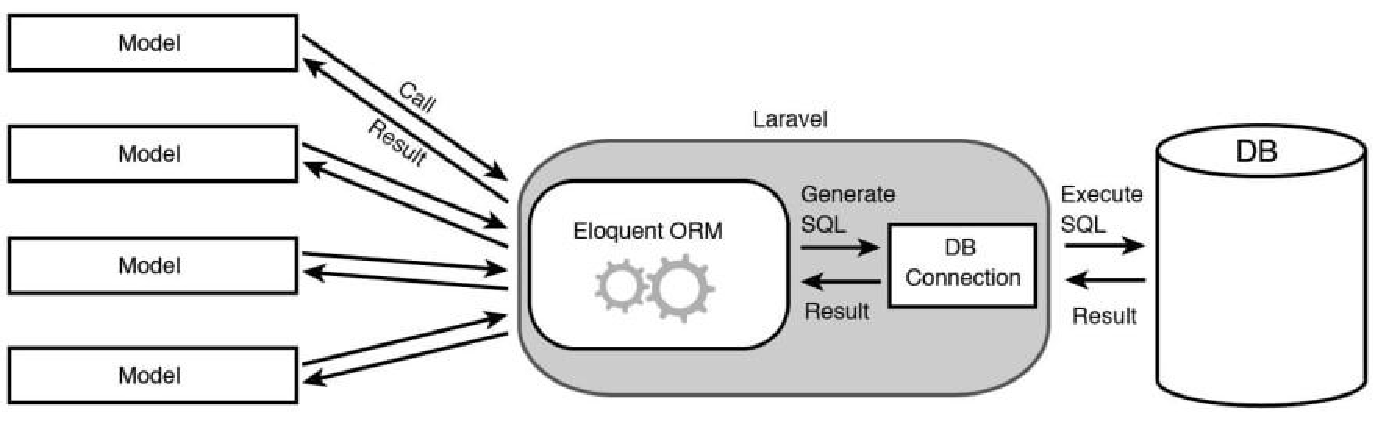
\includegraphics[width=0.6\linewidth]{webinterface/eloquent_workflow.pdf}
  \caption{Eloquent ORM Workflow von \citeurl[]{eloquentworkflow}}
\end{figure}

\paragraph{Laravel Sanctum}\mbox{}\\
Laravel Sanctum ist ein First-Party-Package von den Entwicklern von Laravel und
ermöglicht eine einfache Authentifizierung mithilfe von API-Tokens. Dabei wird
der vom Benutzer erstellte API-Token im HTTP Header \verb|Authorization|
mitgeliefert und somit autorisiert. Da es sich hierbei um ein
Sicherheitskritisches Modul handelt ist es besonders wichtig, dass dieser Code
nahezu Fehlerfrei ist und dies wird durch kontinuierliche Updates und Patches
garantiert.
 
\paragraph{Sessions}\mbox{}\\
Das HTTP Netzwerkprotokoll ist ein Zustandsloses Protokoll, da aber immer über
einen Benutzer Informationen über mehrere Seiten beibehalten werden sollen wird
ein System benötigt um diese Informationen zu speichern. Sessions lösen dieses
Problem und funktionieren wie folgt. Ein Benutzer besucht eine Seite und besitzt
im lokalen Speicher (Cookie) eine Session ID vom Server. Wenn der Benutzer nun
eine andere Seite der gleichen Webseite besucht wird diese Session ID dem Server
wieder gesendet und er kann den Benutzer zuordnen. Laravel verwendet als Backend
für die Sessions Memcached oder Redis.

\paragraph{Middleware}\mbox{}\\
Eine Middleware erleichtert es HTTP Anfragen zu filtern bzw. zu begutachten.
Beispielsweise wird im Webinterface eine Middleware für das richtige setzen der
Sprache verwendet. Bei jedem Aufruf einer Seite überprüft die Middleware welcher
Wert in der Sessions des Benutzers steht um so die passende Sprache auszuwählen.

\paragraph{Service Provider}\mbox{}\\
Service Provider sind da um bestimmte Funktionen einer Anwendung zu
initialisieren. Beispielsweise wird im Webinterface ein
\textit{SettingsServerProvider} verwendet um die Einstellungen aus der Datenbank
in das Laravel Einstellungssystem zu übernehmen.

\paragraph{Form Validation}\mbox{}\\
Für bestimmte Formulare ist es notwendig zu überprüfen ob die Angaben korrekt
sind, beispielsweise dass ein Passwort eine bestimmte Länge hat oder ob eine
E-Mail ein @-Zeichen enthält. Um diese HTTP-Anfragen zu überprüfen müssen Regeln
festgelegt, diese werden in Laravel in \textit{Request} Files festgelegt.

\begin{listing}[H]
  \begin{minted}{php}
    <?php
    public function rules()
    {
      return [
        'first_name' => ['string', 'max:255'],
        'last_name' => ['string', 'max:255'],
        'email' => ['string', 'email', 'max:255'],
        'password' => ['nullable', 'string', 'min:8', 'confirmed'],
      ];
    }
  \end{minted}
  \caption{UserUpdate Request}
  \label{lst:userupdate_request}
\end{listing}

Im Code~\ref{lst:userupdate_request} werden Regeln für den Vornamen, Nachnamen,
die Email und für das Passwort festgelegt. Die verfügbaren Regeln sind durch
Laravel definiert. Liefert eine Request Methode \textit{false} wird der
Controller nicht weiter ausgeführt und die nicht korrekt ausgefüllten Felder
werden in der Session gespeichert und können dem User als Fehlernachricht
dargestellt werden.



\subsection{Lokale Entwicklungsumgebung mit Laragon}
Für die Programmierung des Webinterfaces müssen zuerst einige Vorkehrungen
getroffen werden, dazu zählt zu einem die Installation von benötigter Software
und deren konfiguration.

\subsubsection{Benötigte Software}

\begin{itemize}
  \item \textbf{Laragon} (\url{https://laragon.org}) \\Beinhaltet mehrere
        Softwarepakete die für die Entwicklung notwendig sind.
        \begin{itemize}
          \item Apache HTTP Server
          \item MySQL
          \item PHP
        \end{itemize}
  \item \textbf{phpMyAdmin} (\url{https://www.phpmyadmin.net}) \\ Webinterface
        für MySQL
  \item \textbf{Composer} (\url{https://getcomposer.org}) \\ Paketmanager für
        PHP
  \item \textbf{Git} (\url{https://git-scm.com}) \\ Versionskontrolle
  \item \textbf{Visual Studio Code} (\url{https://code.visualstudio.com}) \\
        Quelltext-Editor
\end{itemize}


\subsubsection{Konfiguration von PHP}
Um PHP Befehle von der Kommandozeile auszuführen muss die Installation zuerst in
den Windows Path Variables hinzugefügt werden.

Dies erfolgt durch die \verb|Advanced System Settings| $\blacktriangleright$
\verb|Environment Variables| $\blacktriangleright$ \verb|System Variables|. Dort
kann nun die Path Variable editiert werden und der Pfad hinzugefügt werden in
welchem die \verb|php.exe| liegt.

\begin{figure}[H]
  \centering
  \frame{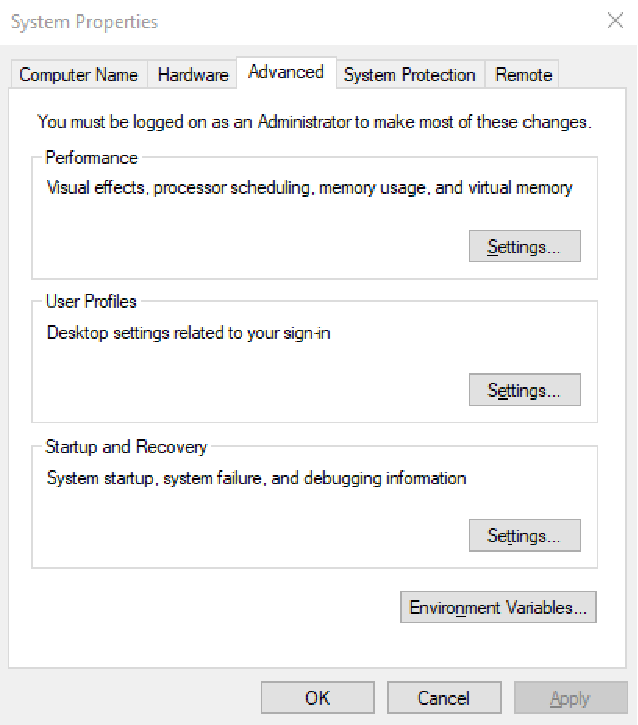
\includegraphics[width=0.6\linewidth]{webinterface/advanced_system_settings.pdf}}
  \caption{Advanced System Settings}
\end{figure}

\begin{figure}[H]
  \centering
  \frame{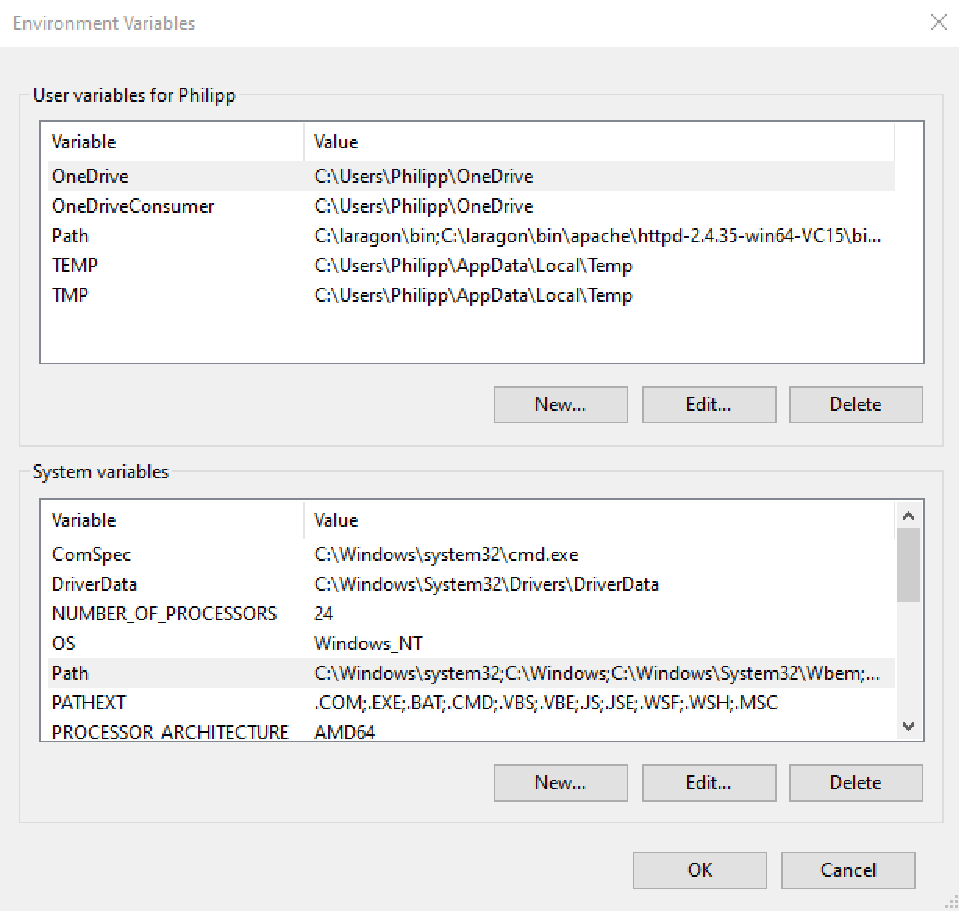
\includegraphics[width=0.6\linewidth]{webinterface/system_variables.pdf}}
  \caption{System Variables}
\end{figure}

\begin{figure}[H]
  \centering
  \frame{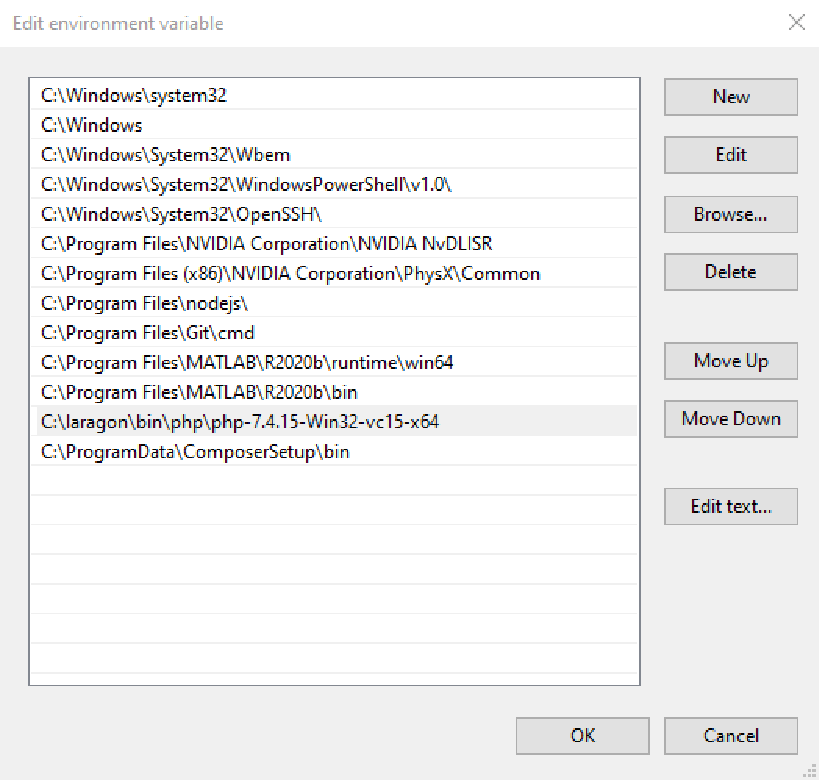
\includegraphics[width=0.6\linewidth]{webinterface/environment_variable.pdf}}
  \caption{Environment Variables}
\end{figure}

Die korrekte konfiguration kann durch die Kommandozeile geprüft werden, dort
muss das Befehl \verb|php -v| ausgeführt werden. Dabei ist zu beachten, dass
nach dem hinzufügen der Path Variable die gewählte Kommandozeile neu gestartet
werden muss.

\begin{figure}[H]
  \centering
  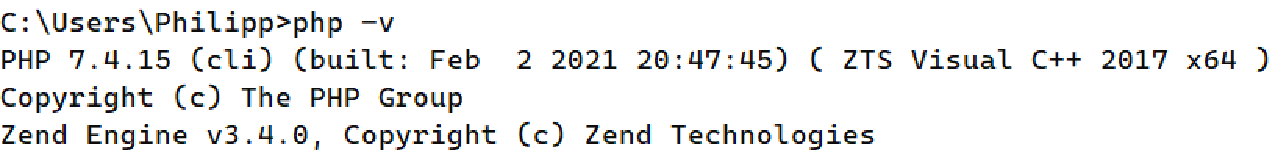
\includegraphics[width=1\linewidth]{webinterface/php_version.pdf}
  \caption{PHP Version}
\end{figure}

Somit ist PHP korrekt konfiguriert.


\subsubsection{Installation von phpMyAdmin}
phpMyAdmin ist ein Tool, welches den Umgang mit MySQL Datenbanken mit einem
Webinterface erleichtert. Die aktuellste Version lässt sich von
\url{https://www.phpmyadmin.net/downloads} downloaden. Dieses Archiv muss
entpackt werden und ausgehend vom Laragon Root Verzeichnis in das Verzeichnis
\verb|/etc/apps| kopiert werden. Um die Installation zu überprüfen muss der
Apache HTTP Server und der MySQL Server gestartet werden, nun sollte bei einer
korrekten Installation das Webinterface von phpMyAdmin unter
\url{http://localhost/phpmyadmin} erreichbar sein.

\begin{figure}[H]
  \centering
  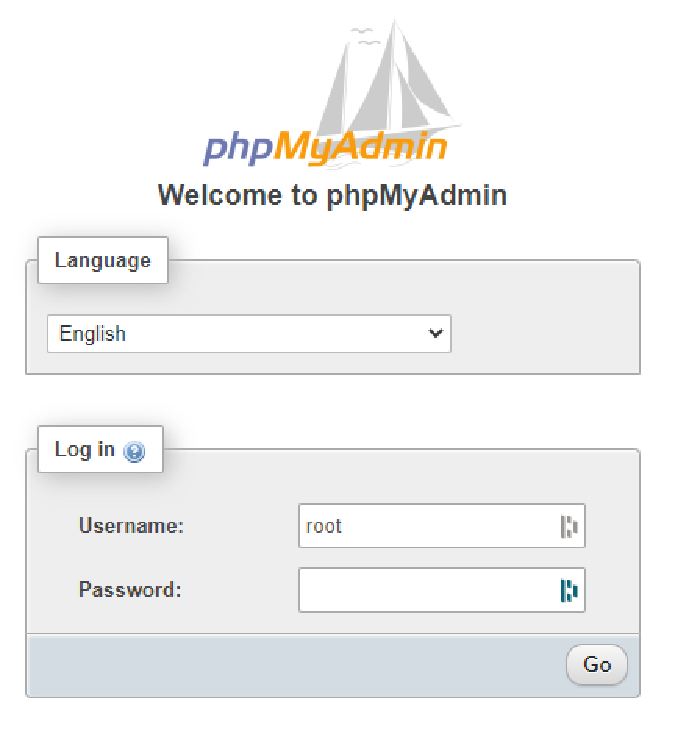
\includegraphics[width=0.5\linewidth]{webinterface/phpmyadmin.pdf}
  \caption{phpMyAdmin Webinterface}
\end{figure}

Es ist nicht notwendig ein Passwort einzugeben, da Standardmäßig kein Passwort
gesetzt wird.


\subsection{Lokale Entwicklungsumgebung mit WSL und Docker}


\subsubsection{Benötigte Software}

\begin{itemize}
  \item \textbf{Docker} (\url{https://www.docker.com}) \\ Ermöglicht Isolation
        von Anwendungen mit Containervirtualisierung
  \item \textbf{WSL} (\url{https://docs.microsoft.com/en-us/windows/wsl}) \\
        Kompatibilitätsschicht für Linux Anwendungen unter Windows 10
  \item \textbf{Visual Studio Code} (\url{https://code.visualstudio.com}) \\
        Quelltext-Editor
\end{itemize}


\subsubsection{Installation von WSL}
Zuerst müssen einige Einstellungen in Windows getroffen werden um später eine
Linux Distribution herunterzuladen können. Diese Befehle können über die
Kommandozeile mit Administrativen Rechten ausgeführt werden.

\begin{listing}[H]
  \begin{minted}{bash}
    dism.exe /online /enable-feature /featurename:Microsoft-Windows-Subsystem-Linux /all /norestart
  \end{minted}
  \caption{WSL Feature Feature aktivierens}
\end{listing}

\paragraph{2. Schritt: Virtual Machine Aktivieren}\mbox{}\\
\begin{listing}[H]
  \begin{minted}{bash}
    dism.exe /online /enable-feature /featurename:VirtualMachinePlatform /all /norestart
  \end{minted}
  \caption{Virtual Machine Feature aktivieren}
\end{listing}

Nach diesem Schritt ist ein Neustart des Computers notwendig.

\paragraph{3. Schritt: Linux Kernel Update}\mbox{}\\
Nun muss ein Linux Kernel Update installiert werden, die aktuelle Version ist
unter \url{https://aka.ms/wsl2kernel} zu finden.

\paragraph{4. Schritt: WSL 2}\mbox{}\\
Nach dem Neustart des Computers sollte es nun möglich sein WSL 2 als Version
auszuwählen.
\begin{listing}[H]
  \begin{minted}{bash}
    wsl --set-default-version 2
  \end{minted}
  \caption{WSL 2 auswählen}
\end{listing}

\paragraph{5. Schritt: Linux Distribution herunterladen}\mbox{}\\
Zuletzt kann eine Linux Distribution aus dem Windows Store heruntergeladen
werden, in diesem Fall Debian (\url{https://www.microsoft.com/de-de/p/debian}).


\subsubsection{Installation von Docker}
Die aktuellste Version von Docker Desktop für Windows lässt sich am einfachsten
über die offizielle Website von Docker herunterladen (\url{https://docker.com}).
Nach der Installation muss noch die WSL Integration aktiviert werden. Dazu muss
in den Einstellungen unter \verb|Resources| $\blacktriangleright$ \verb|WSL Integration|
und dort muss der Haken bei \textit{Enable integration with my default WSL distro}
gesetzt werden und die installierte Linux Distribution muss unten aktiviert
werden.

\begin{figure}[H]
  \centering
  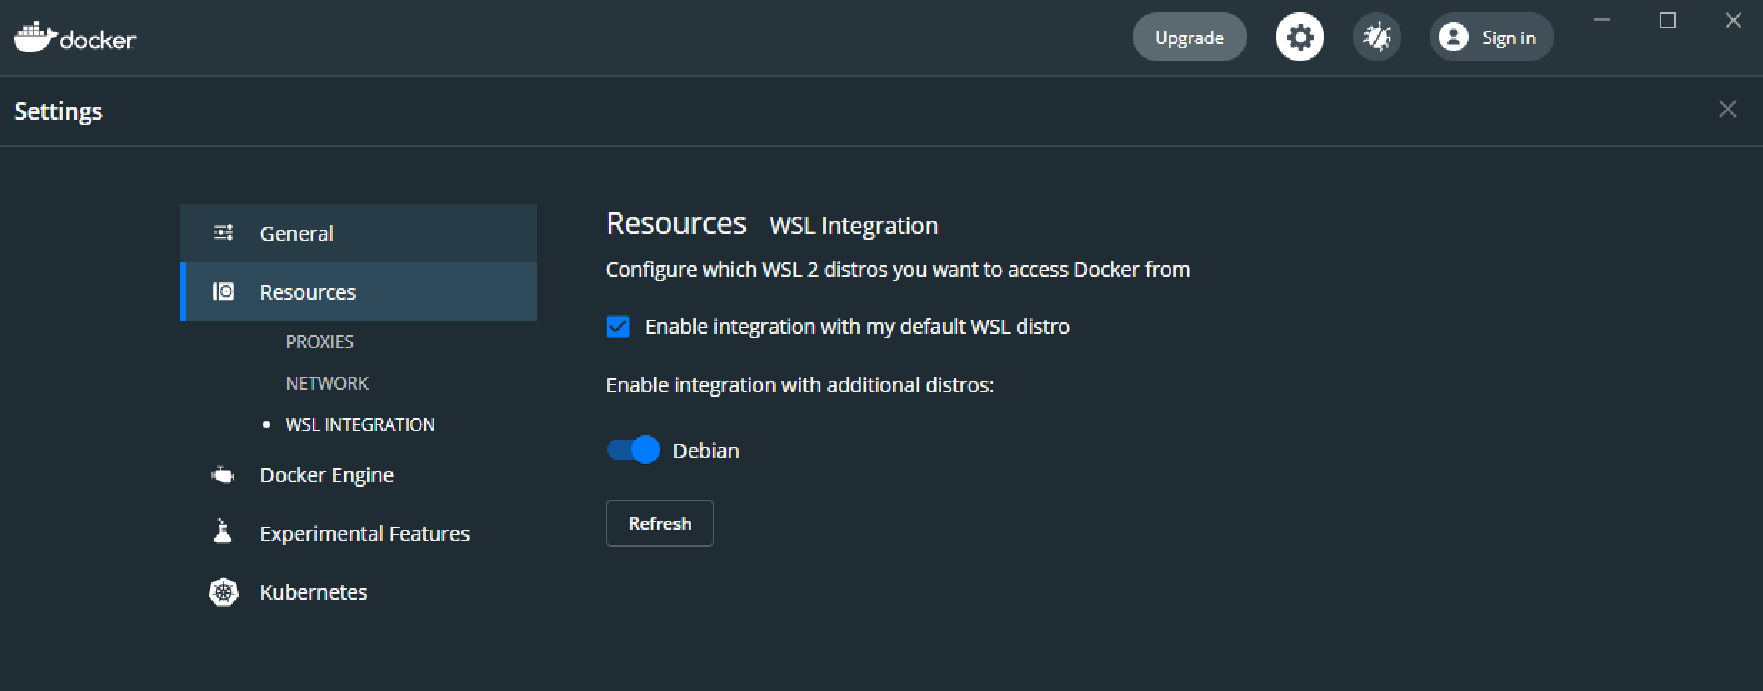
\includegraphics[width=1\linewidth]{webinterface/docker.pdf}
  \caption{Docker WSL Integration}
\end{figure}

Somit ist die Lokale Entwicklungsumgebung mit WSL und Docker abgeschlossen, die
benötigte Software wird später automatisch durch Laravel Sail in einem Docker
Container installiert.

\begin{figure}[H]
  \centering
  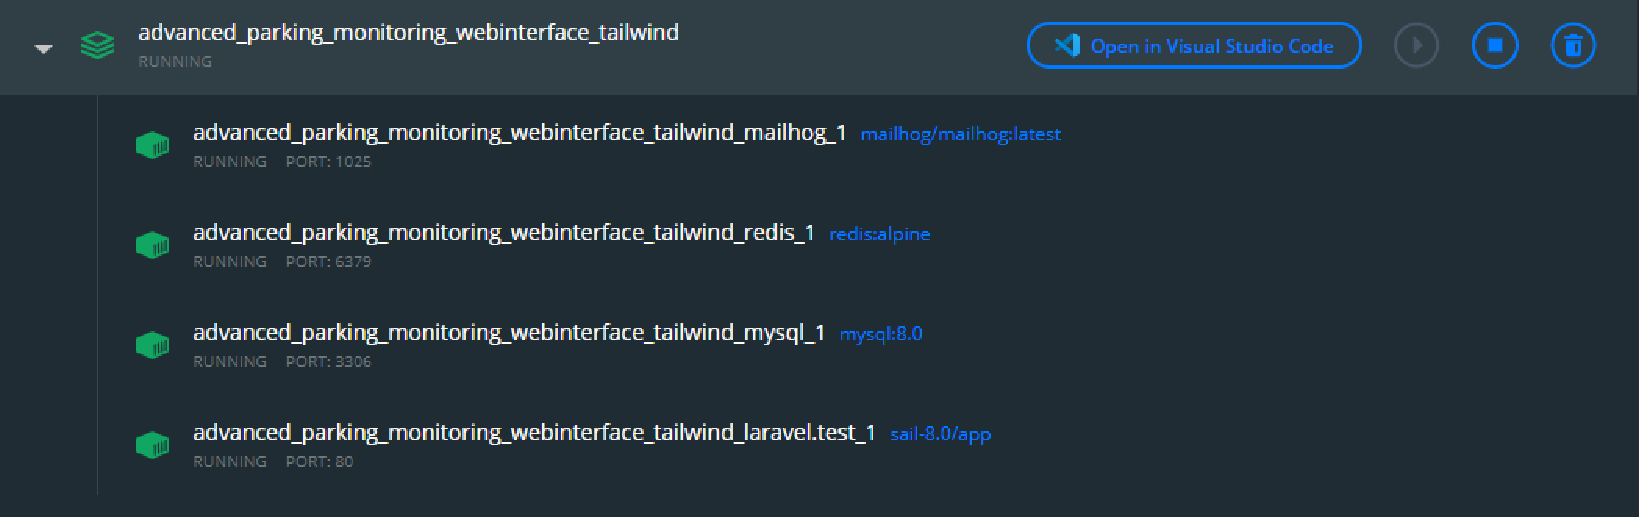
\includegraphics[width=1\linewidth]{webinterface/docker_container.pdf}
  \caption{Docker Container Steuerung}
\end{figure}

Es ist somit möglich die Services welche im Container in der Linux Distribution
laufen über die Docker Desktop Anwendung zu steuern.


\subsection{Production Server}
Der Production Server bzw. der Live Server ist der Server wo sich die
Webanwendung befindet und die Endbenutzer zugreifen, dieser Server wird auch
einfach mit Production abgekürzt. Der Production Server ist in diesem Fall ein
Virtual Private Server mit dem Betriebsystem Debian 10, welcher bei einem
Internet-Hosting Unternehmen mit Sitz in Deutschland gehostet wird.


\subsubsection{Benötigte Software}

Für den Live Server wird der sogenannte \glqq LAMP\grqq{} Stack verwendet. LAMP steht dabei
für die Software \textbf{L}inux, \textbf{A}pache, \textbf{M}ySQL und \textbf{P}HP.

\begin{itemize}
  \item \textbf{Apache Web Server} (\url{https://httpd.apache.org}) \\ HTTP Server
  \item \textbf{MariaDB} (\url{https://mariadb.org}) \\ Fork von MySQL
  \item \textbf{PHP} (\url{https://www.php.net}) \\ \ac*{PHP}
  \item \textbf{phpMyAdmin} (\url{https://www.phpmyadmin.net}) \\ Webinterface
        für MySQL
  \item \textbf{Composer} (\url{https://getcomposer.org}) \\ Paketmanager für PHP
  \item \textbf{Git} (\url{https://git-scm.com}) \\ Versionskontrolle
\end{itemize}


\subsubsection{Installation des LAMP Stacks}
Bevor die Software Pakete installiert werden sollte die Linux Software/Update
Repository geupdatet werden.

\begin{listing}[H]
  \begin{minted}{bash}
    apt-get update && apt-get upgrade
  \end{minted}
  \caption{Respositorys updaten}
\end{listing}

\paragraph{Apache}\mbox{}\\

Nun kann der Apache Web Server installiert werden.

\begin{listing}[H]
  \begin{minted}{bash}
    apt install apache2
  \end{minted}
  \caption{Apache installieren}
\end{listing}

Die Installation kann nun leicht überprüft werden indem man im Browser die IP
bzw. die dazugehörige Domain öffnet, in diesem Fall:
(\url{http://dev.philipp-kraft.com}).

\begin{figure}[H]
  \centering
  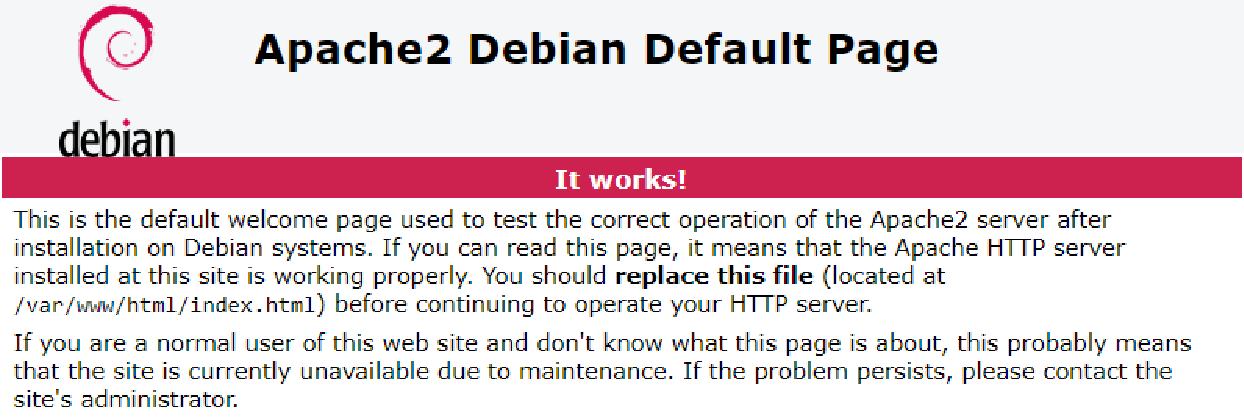
\includegraphics[width=1\linewidth]{webinterface/apache2_installation.pdf}
  \caption{Debian Default Page}
\end{figure}

Erscheint die Debian Default Page ist Apache korrekt installiert.

\paragraph{PHP}\mbox{}\\
Neben PHP werden auch einige PHP Extensions benötigt.

\begin{listing}[H]
  \begin{minted}{bash}
    apt install wget php php-cgi php-mysqli php-pear php-mbstring php-gettext libapache2-mod-php php-common php-phpseclib php-mysql
  \end{minted}
  \caption{PHP installieren}
\end{listing}

Die Installation kann einfach mit dem Befehl \verb|php -v| überprüft werden.

\paragraph{MariaDB}\mbox{}\\

\begin{listing}[H]
  \begin{minted}{bash}
    apt install mariadb-server
  \end{minted}
  \caption{MariadB installieren}
\end{listing}

Nun muss MariaDB noch konfiguriert werden.

\begin{listing}[H]
  \begin{minted}{bash}
    mysql_secure_installation
  \end{minted}
  \caption{MariaDB Secure Installation}
\end{listing}

Dabei wird dem root MySQL User ein Passwort gesetzt, Anonyme Benutzer gelöscht
und es werden Test Datenbanken gelöscht.

Nun wird ein neuer Benutzer mit root Berechtigungen erstellt.

\begin{listing}[H]
  \begin{minted}{sql}
    mysql
    GRANT ALL ON *.* TO 'admin'@'localhost' IDENTIFIED 
    BY 'password' WITH GRANT OPTION;
    flush privileges;
    exit
  \end{minted}
  \caption{MariaDB konfiguration}
\end{listing}

\paragraph{phpMyAdmin}\mbox{}\\

Die aktuelle Version von phpMyAdmin kann von
(\url{https://www.phpmyadmin.net/downloads}) bezogen werden und mit dem
\verb|wget| Befehl heruntergeladen werden.

\begin{listing}[H]
  \begin{minted}{bash}
    wget https://files.phpmyadmin.net/phpMyAdmin/5.0.4
    /phpMyAdmin-5.0.4-all-languages.tar.gz
  \end{minted}
  \caption{phpMyAdmin Download}
\end{listing}

Anschließend muss das Archiv entpackt werden.

\begin{listing}[H]
  \begin{minted}{bash}
    tar xvf phpMyAdmin-5.0.4-all-languages.tar.gz
  \end{minted}
  \caption{phpMyAdmin Entpacken}
\end{listing}

Als nächstes muss das entpackte Archiv in einen anderen Pfad verschoben werden
und zusätzlich müssen einige Rechte und Verzeichnisse angepasst werden.

\begin{listing}[H]
  \begin{minted}{bash}
    mv phpMyAdmin-5.0.4-all-languages /usr/share/phpmyadmin
    mkdir -p /var/lib/phpmyadmin/tmp
    chown -R www-data:www-data /var/lib/phpmyadmin
    mkdir /etc/phpmyadmin/
  \end{minted}
  \caption{phpMyAdmin Rechte und Verzeichnisse}
\end{listing}

Nun muss eine Konfigurations Datei erstellt werden und dort muss ein Blowfish
Secret\footnote{32 Zeichen String für Cookie-Authentifizierung} angegeben werden
und den Pfad für ein Temporäres Verzeichnis.

\begin{listing}[H]
  \begin{minted}{bash}
    cp /usr/share/phpmyadmin/config.sample.inc.php /usr/share/phpmyadmin/config.inc.php
  \end{minted}
  \caption{phpMyAdmin Konfigurationsdatei erstellen}
\end{listing}

und am Ende dieser Datei müssen folgende zwei Zeilen eingefügt werden.

\begin{listing}[H]
  \begin{minted}{bash}
    $cfg['blowfish_secret'] = 'H2OxcGXxflSd8JwrwVlh6KW6s2rER63i'; 
    $cfg['TempDir'] = '/var/lib/phpmyadmin/tmp';
  \end{minted}
  \caption{phpMyAdmin Blowfish Secret und TempDir}
\end{listing}

Zuletzt muss der Apache Web Server konfiguriert werden.

Im Verzeichnis \verb|/etc/apache2/sites-available| muss eine neue Konfiguration
angelegt werden \verb|phpmyadmin.conf|.

\begin{listing}[H]
  \begin{minted}{bash}
    Listen 9000

    <VirtualHost *:9000>
            ServerName localhost
    
            <Directory /usr/share/phpmyadmin>
                    AllowOverride None
                    Require all granted
            </Directory>
    
            DocumentRoot /usr/share/phpmyadmin
    
            ErrorLog ${APACHE_LOG_DIR}/phpmyadmin.error.log
            CustomLog ${APACHE_LOG_DIR}/phpmyadmin.access.log combined
    </VirtualHost>
  \end{minted}
  \caption{phpmyadmin.conf}
\end{listing}

Nun kann diese Virtual Host Konfigurations Datei aktiviert werden und danach
muss der Apache Web Server neu gestartet werden.

\begin{listing}[H]
  \begin{minted}{bash}
    a2ensite phpmyadmin
    systemctl restart apache2
  \end{minted}
  \caption{Virtual Host aktivieren}
\end{listing}

Diese Konfiguration ermöglicht es, dass das Webinterface von phpMyAdmin über den
Port 9000 (\url{http://dev.philipp-kraft.com:9000}) erreichbar ist und nicht wie
Standardmäßig vorgesehen über das Verzeichnis /phpmyadmin
(\url{http://dev.philipp-kraft.com/phpmyadmin}), dies bietet einen
Sicherheitsvorteil.

\paragraph{Webinterface Virtual Host}\mbox{}\\

Nun muss noch eine Virtual Host Konfiguration für das Webinterface selbst
erstellt werden.

\begin{listing}[H]
  \begin{minted}{bash}
    <VirtualHost *:80>
    ServerAdmin webmaster@localhost
    DocumentRoot /var/www/apm/public
          
    <Directory />
      Options FollowSymLinks
      AllowOverride All
    </Directory>
  
    <Directory /var/www/apm>
      Options Indexes FollowSymLinks MultiViews
      AllowOverride All
      Order allow,deny
      allow from all
    </Directory>
  
    ErrorLog ${APACHE_LOG_DIR}/error.log
    CustomLog ${APACHE_LOG_DIR}/access.log combined
  </VirtualHost>
  \end{minted}
  \caption{apm.conf}
\end{listing}

Diesmal wird auf den Standard HTTP Port 80 gehört und dieser führt in das
Verzeichnis \verb|/var/www/apm/public|. Zusätzlich werden noch Directives
gesetzt, damit das Standard \verb|.htaccess| File von Laravel richtig
funktionieren kann.

\paragraph{Installation von Composer}\mbox{}\\

Die Installation von Composer gestaltet sich relativ einfach.

\begin{listing}[H]
  \begin{minted}{bash}
    wget -O composer-setup.php https://getcomposer.org/installer
  \end{minted}
  \caption{Download Composer Installer}
\end{listing}

Nun muss das Setup ausgeführt werden und damit das \verb|composer| Befehl Global
verfügbar ist wird Composer in den Pfad \verb|/usr/local/bin| verschoben.

\begin{listing}[H]
  \begin{minted}{bash}
    php composer-setup.php --install-dir=/usr/local/bin --filename=composer
  \end{minted}
  \caption{Composer Setup}
\end{listing}


\subsubsection{Deployment mit Github Actions}
Unter Deployment versteht man die automatische Installation von Software, in
diesem Fall auf einem Linux Server. Erreicht wird das durch zwei Bash Scripts
und mit Github Actions (\url{https://github.com/features/actions}).

\paragraph{Git Setup}\mbox{}\\

Sollte auf dem Server noch kein Git installiert sein, lässt sich das wie folgt
installieren.

\begin{listing}[H]
  \begin{minted}{bash}
    apt install git
  \end{minted}
  \caption{Git Installation}
\end{listing}

Im Verzeichnis \verb|/var/www/apm| soll sich später das Webinterface befinden,
deshalb muss in diesem Pfad Git konfiguriert werden. Dazu wird die Remote URL
konfiguriert.

\begin{listing}[H]
  \begin{minted}{bash}
    git config remote.origin.url 'https://{TOKEN}@github.com/
    Philipp-Kraft/Advanced_Parking_Monitoring_Webinterface.git'
  \end{minted}
  \caption{Git Remote Origin}
\end{listing}

Da beim Github Account eine Zwei-Faktor-Authentisierung verwendet wird muss die
Authentifizierung mit einem Personal access token erfolgen. Dieser kann unter
\url{https://github.com/settings/tokens} erstellt werden, der erstellte Token
kann dann einfach in der URL eingefügt werden.

\paragraph{Deploy Script}\mbox{}\\

Das Deploy-Script wird auf der Lokalen Entwicklermaschine ausgeführt. Das Script
wechselt in den Production Branch und merged mit dem Main Branch, dieser Push in
den Production Branch löst dann die Github Action aus.

\begin{listing}[H]
  \begin{minted}{bash}
    #!/bin/sh
    set -e
    
    #vendor/bin/phpunit
    
    (git push) || true
    
    git checkout production
    git merge main
    
    git push origin production
    
    git checkout main
  \end{minted}
  \caption{deploy.sh}
\end{listing}

\paragraph{Server Deploy Script}\mbox{}\\

Das Server Deploy Script \verb|server_deploy.sh| versetzt die Laravel
Applikation in den Wartungsmodus und lädt sich vom deploy Branch den Code auf
den Server herunter, danach werden einige Befehle ausgeführt.

\begin{longlisting}
  \begin{minted}{bash}
    #!/bin/sh
    set -e
    
    echo "Deploying application ..."
    
    # Enter maintenance mode
    php artisan down
        
        # Update codebase
        git fetch origin deploy
        git reset --hard origin/deploy
    
        # Install dependencies based on lock file
        composer install --no-interaction --prefer-dist --optimize-autoloader
    
        # Migrate database
        php artisan migrate:refresh --seed
    
        # Clear cache
        php artisan optimize
    
    # Exit maintenance mode
    php artisan up
    
    echo "Application deployed!"
  \end{minted}
  \caption{serverdeploy.sh}
\end{longlisting}


\paragraph{Github Action}\mbox{}\\
Github Actions ist ein Projekt von Github, welches es ermöglicht
Automatisierungen in den Bereichen Entwicklung, Testing und Deployment
durchzuführen.

Als erstes muss ein Workflow erstellt werden, dieser wird im Root-Verzeichnis
des Projekts erstellt \verb|APM\.github\workflows\main.yml|.

\begin{longlisting}
  \begin{minted}{bash}
    name: Deploy Laravel app

    on:
      push:
        branches: [ production ]
    
    jobs:
      deploy:
        runs-on: ubuntu-latest
        steps:
        - uses: actions/checkout@v2
          with:
            token: ${{ secrets.PUSH_TOKEN }}
        - name: Set up Node
          uses: actions/setup-node@v1
          with:
            node-version: '12.x'
        - run: npm install
        - run: npm run production
        - name: Commit built assets
          run: |
            git config --local user.email "action@github.com"
            git config --local user.name "GitHub Action"
            git checkout -B deploy
            git add -f public/
            git commit -m "Build front-end assets"
            git push -f origin deploy
        - name: Deploy to production
          uses: appleboy/ssh-action@master
          with:
            username: root
            host: dev.philipp-kraft.com
            password: ${{ secrets.SSH_PASSWORD }}
            script: 'cd /var/apm && ./server_deploy.sh && chown -R www-data.www-data /var/apm && chmod -R 755 /var/apm && chmod -R 777 /var/apm/storage' 
  \end{minted}
  \caption{main.yml}
\end{longlisting}

Dieser Workflow setzt einen Ubuntu Server in der Cloud auf und baut dort die
Assets zusammen, damit die Downtime auf dem Production Server möglichst gering
ist. Danach wird eine SSH Verbindung zum Production Server aufgebaut und dort
wird das Bash-Script \verb|server_deploy.sh| ausgeführt. Gleichzeitig werden
einige Berechtigungen angepasst.

In der Repository muss nun noch das SSH-Passwort und der Personal access token
hinterlegt werden. Dies geschieht über \verb|Settings| $\blacktriangleright$
\verb|Secrets|. Dort können nun über \verb|New respository secrets| die Secrets
hinterlegt werden.

\begin{figure}[H]
  \centering
  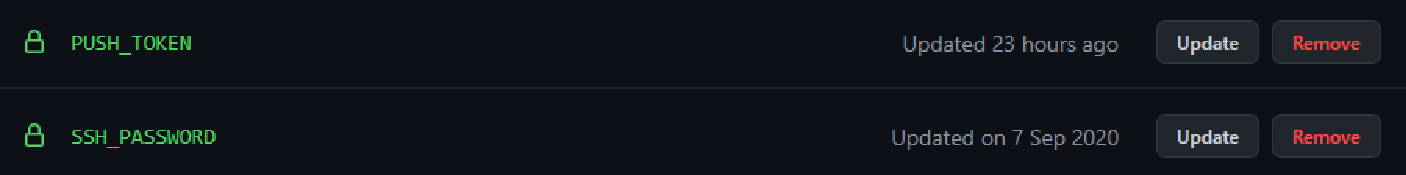
\includegraphics[width=1\linewidth]{webinterface/action_secrets.pdf}
  \caption{Action Secrets}
\end{figure}

\begin{figure}[H]
  \centering
  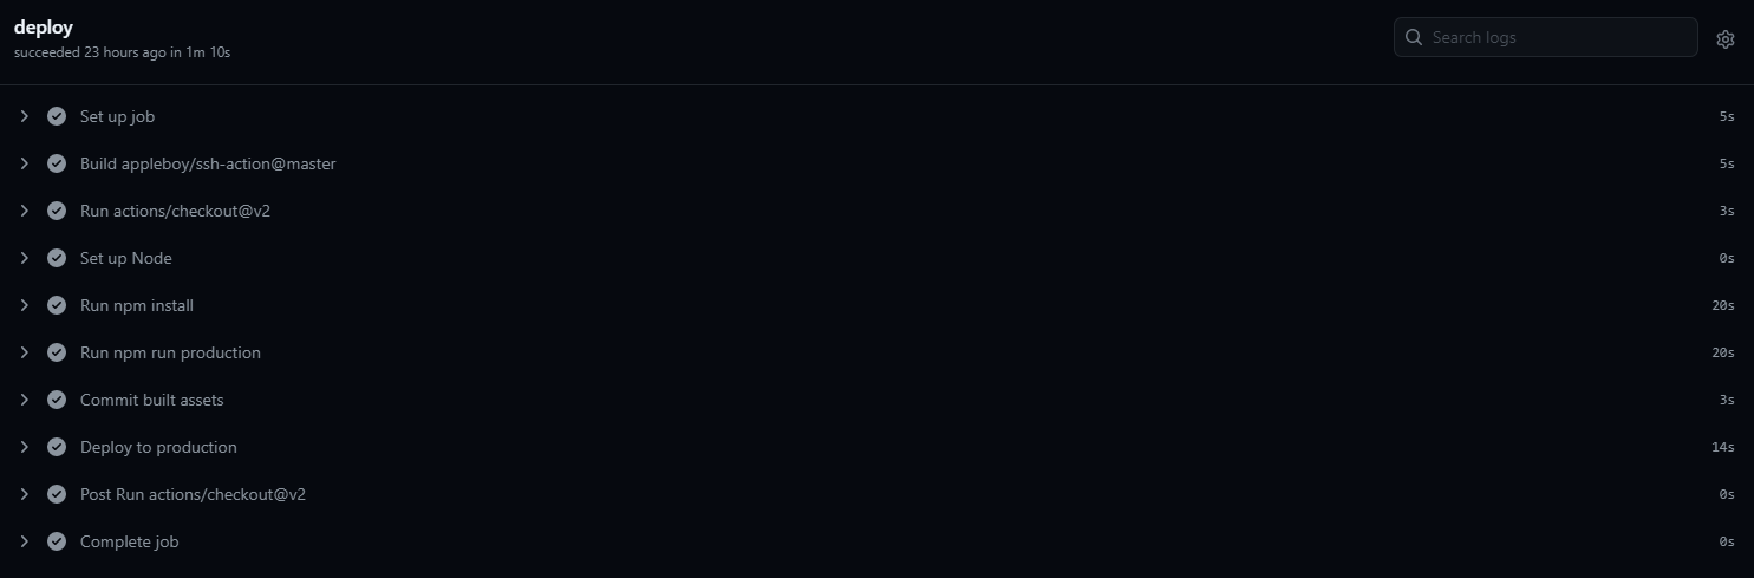
\includegraphics[width=1\linewidth]{webinterface/github_deploy.pdf}
  \caption{Github Action Übersicht}
\end{figure}


\subsection{Grundlegender Aufbau Frontend}

Da das Ziel ist, dass das Frontend des Webinterfaces möglichst Modular aufgebaut ist
und so wenig Code wie möglich wiederholt wird. Ermöglicht wird dies durch das
aufbauen der Seite mithilfe von Components.


\subsubsection{Components}

Components sind praktisch kleine Bausteine aus denen die komplette Seite
aufgebaut ist. Components sind kein natives Feature von HTML/CSS oder PHP, diese
Funktion wird von der Template Engine Blade bereitgestellt, deshalb werden diese
auch oft Blade Components genannt. 

\paragraph{Anonymous Components}\mbox{}\\

Es gibt viele verschiedene Möglichkeiten Components zu erstellen und
verschiedene Konventionen am, einfachsten sind aber die \textit{Anonymous Components}, 
diese haben den Vorteil, dass diese in einer Datei verwaltet werden
können und somit sehr einfach zu handhaben sind.

\paragraph{Components erstellen}\mbox{}\\

Das Erstellen von einem Component wird nun anhand eines Buttons gezeigt. Da
dieser als Anonymous Component angelegt wird muss dieser mit keiner Klasse
assoziiert werden, es wird einfach im Pfad \verb|resources\views\components| ein
Ordner mit dem Namen \verb|buttons| angelegt und darin ein Blade File mit dem
Namen \verb|primary.blade.php|. Dort kann nun der gewünschte HTML Code platziert
werden.

\begin{listing}[H]
  \begin{minted}{html}
    <button type="submit" class="inline-flex items-center px-4 py-2 bg-apm-blue...">
      {{ $slot }}
    </button>
  \end{minted}
  \caption{primary.blade.php}
  \label{lst:primary.blade.php}
\end{listing}


Im Code~\ref{lst:primary.blade.php} ist eine Variable mit dem Namen \verb|slot|
verwendet worden. Diese Variable wird später beim verwenden automatisch mit dem
Inhalt zwischen dem HTML Element ersetzt.


\paragraph{Components verwenden}\mbox{}\\

Es stellt sich nun die Frage wie man dieses erstelle Component nun verwendet.
Die Blade Components verwenden den gleichen Syntax wie ein normales HTML
Element, mit dem Unterschied dass ein \verb|x-| vor dem Namen des Components
angeführt werden muss. Da sich der vorhin erstellte Component in einem Ordner befindet muss das auch
angegeben werden, dabei wird kein Slash wie üblich um einen Pfad anzugeben
verwendet sondern ein Punkt, es muss auch keine Extensions angegeben werden.

\begin{listing}[H]
  \begin{minted}{html}
    <x-buttons.primary>Press me!</x-buttons.primary>
  \end{minted}
  \caption{Verwendung eines Button Components}
\end{listing}


\paragraph{Attribute übergeben}\mbox{}\\

Auch wenn viele Components ohne Problem überall ohne Veränderung verwendet
werden können, ist es gewünscht bei manchen Components beispielweise eine
zusätzliche Klasse anzugeben um die Größe des Elements zu verändern. Erreicht
wird das mit der \verb|attributes| Variable im Blade File des Components, da
aber oft schon Attribute definiert sind ist es möglich mit der \verb|merge|
Methode die Attribute zusammenzuführen.


\begin{listing}[H]
  \begin{minted}{php}
  <button {{ $attributes->merge(['type' => 'submit], 'class' => 'inline-flex items-center px-4 py-2 bg-apm-blue...') }}>
    {{ $slot }}
  </button>
  \end{minted}
  \caption{Modularer Button Component}
\end{listing}

Somit ist dieser Button Component nun vollständig Modular.


\subsubsection{Layouts}

Da auf den meisten Seiten des Webinterfaces fast das gleiche Layout beibehaltet
ist es sinnvoll diesen Inhalt in ein Component umzuwandeln. Auch Layouts sind
Components.

Es gibt im Webinterface folgende Layouts:

\begin{itemize}
  \item \textbf{app.blade.php}\\
  Layout für Allgemeine Seiten
  \item \textbf{admin.blade.php}\\
  Layout für die Administrativen Seiten mit einer Sidebar und Page Header
  \item \textbf{display.blade.php}\\
  Besonderes Layout für die Display Seiten
\end{itemize}

\begin{figure}[H]
  \centering
  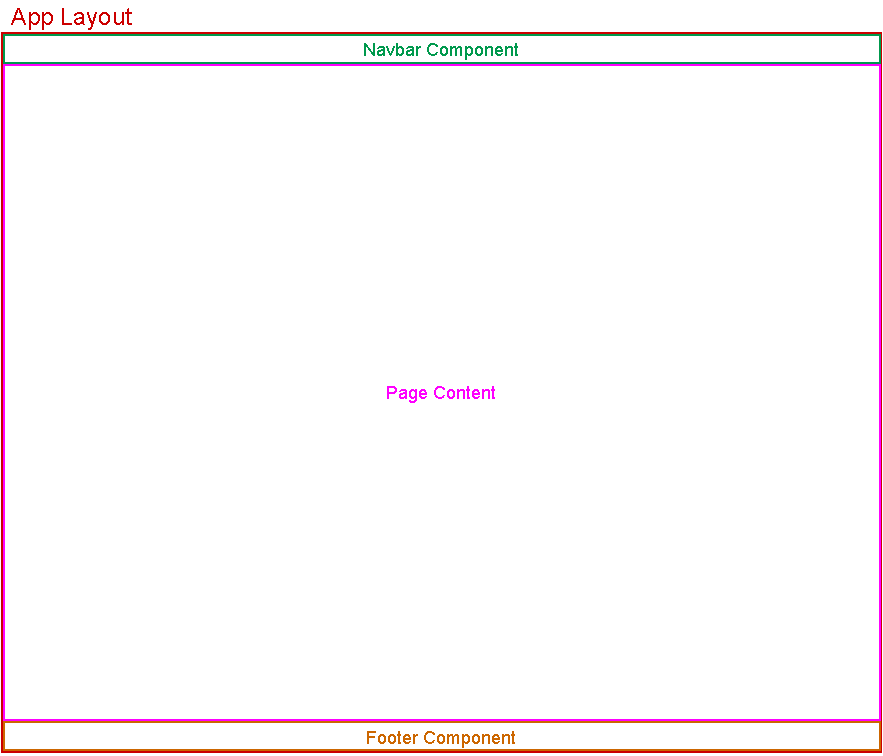
\includegraphics[width=1\linewidth]{webinterface/app_layout.pdf}
  \caption{App Layout}
\end{figure}

Das App Layout ist das Standardmäßige Layout, es besteht aus drei Components,
der Navigation Bar, dem Page Content und aus einem dynamische Footer.

\begin{figure}[H]
  \centering
  \frame{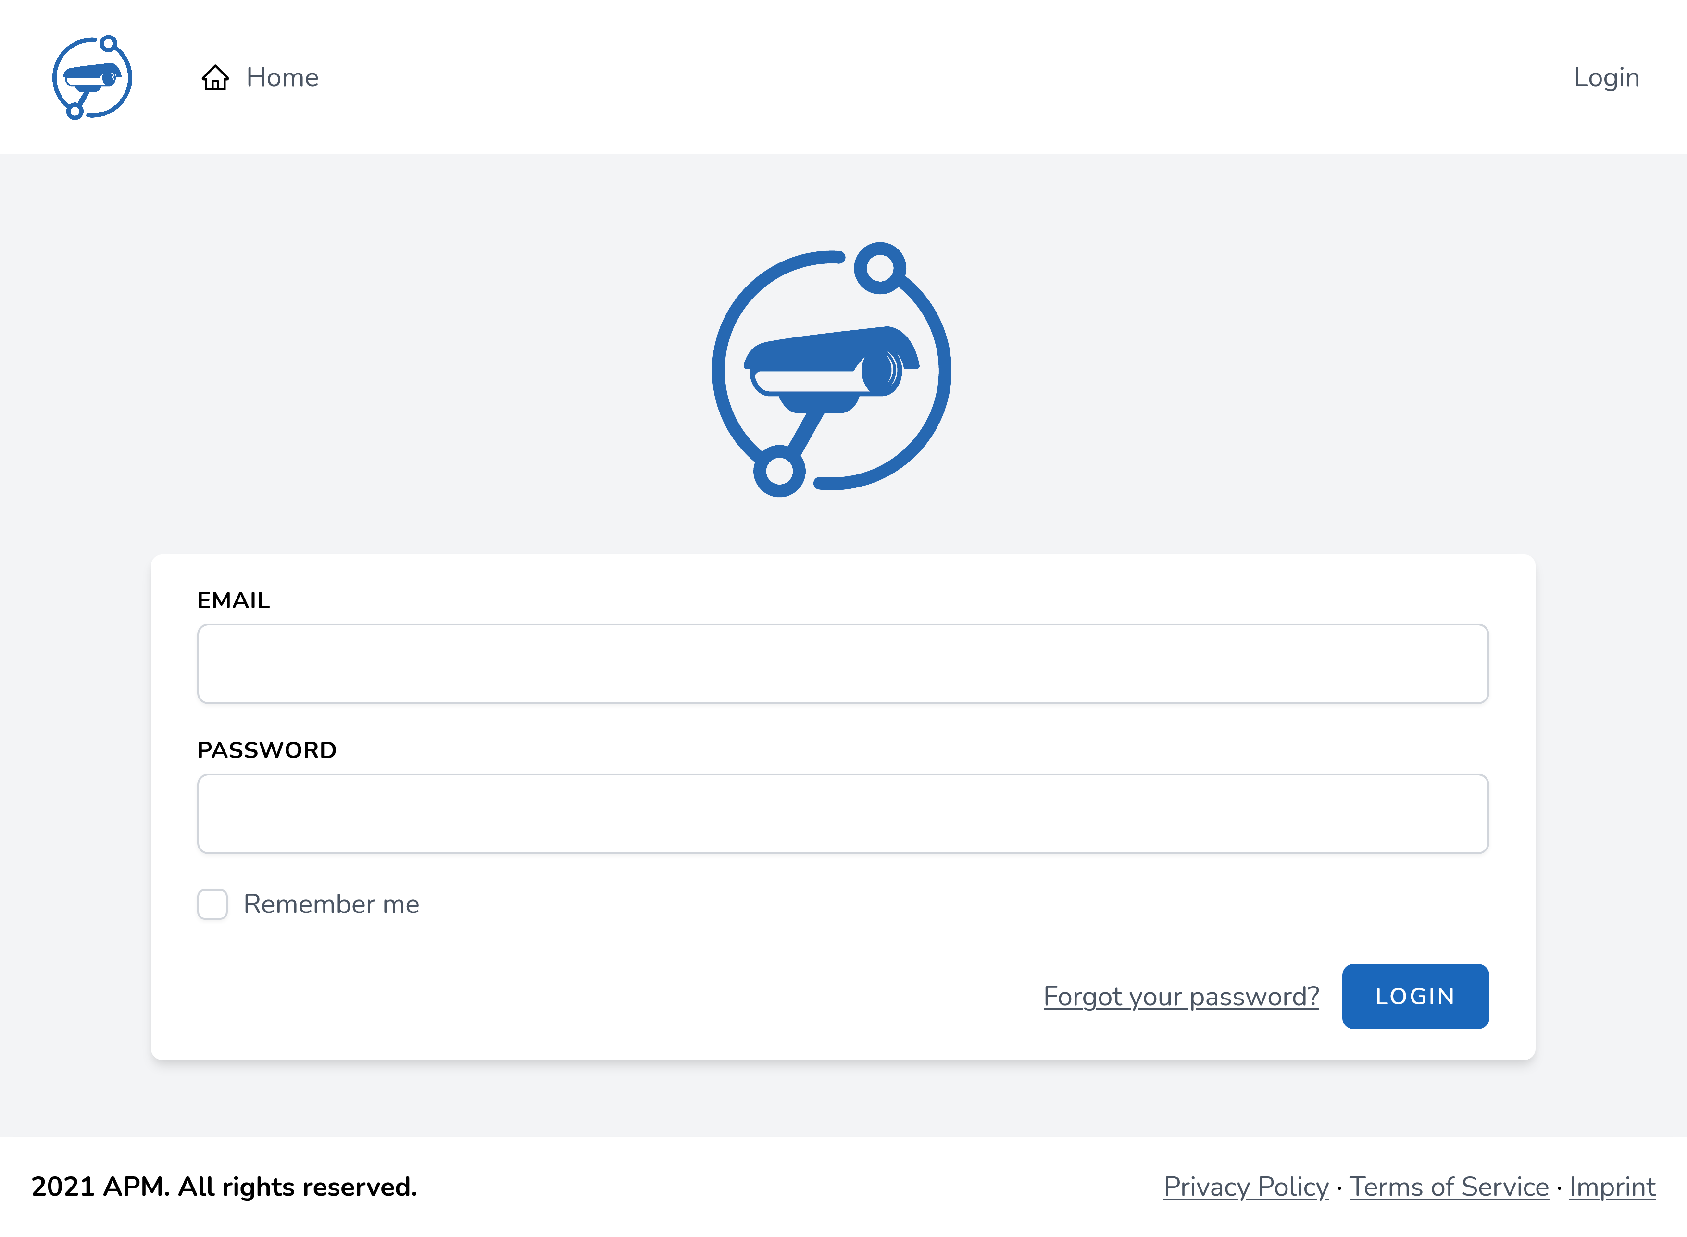
\includegraphics[width=1\linewidth]{webinterface/login_site.pdf}}
  \caption{Login Seite mit App Layout}
  \label{fig:login_site}
\end{figure}

In der Abbildung~\ref{fig:login_site} wird das App Layout verwendet. Dabei sind
die drei Components erkennbar.

\begin{figure}[H]
  \centering
  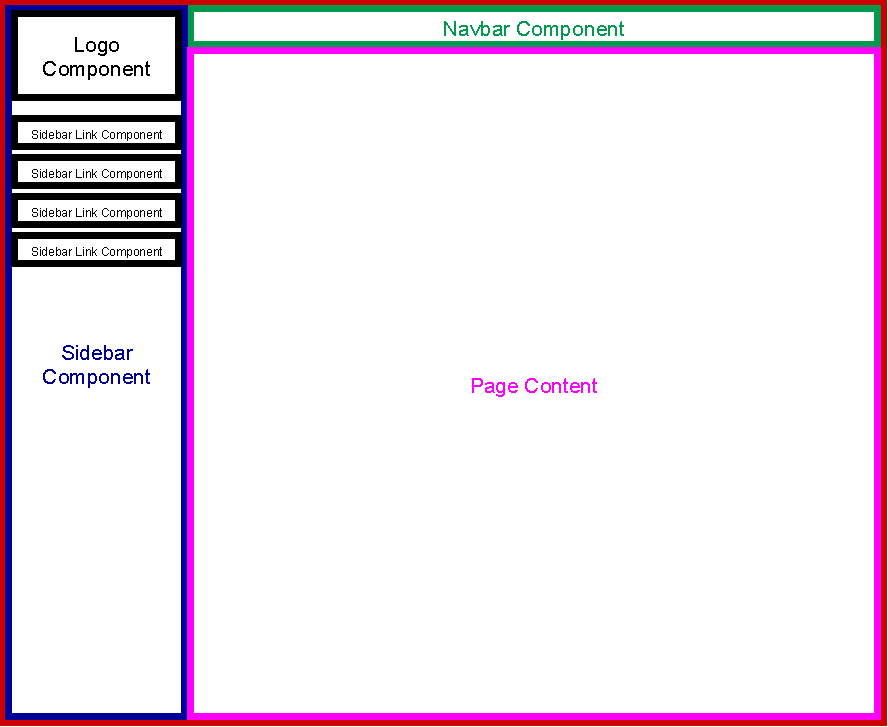
\includegraphics[width=1\linewidth]{webinterface/admin_layout.pdf}
  \caption{Admin Layout}
\end{figure}

Das Admin Layout besitzt eine zusätzliche Sidebar mit Links zu verschiedenen
Administrativen Seiten, im Vergleich zum Standardmäßigen besitzt das Admin
Layout keinen Footer und eine leicht veränderte Navbar\footnote{Navigation Bar
engl. für Navigationsleiste}.

\begin{figure}[H]
  \centering
  \frame{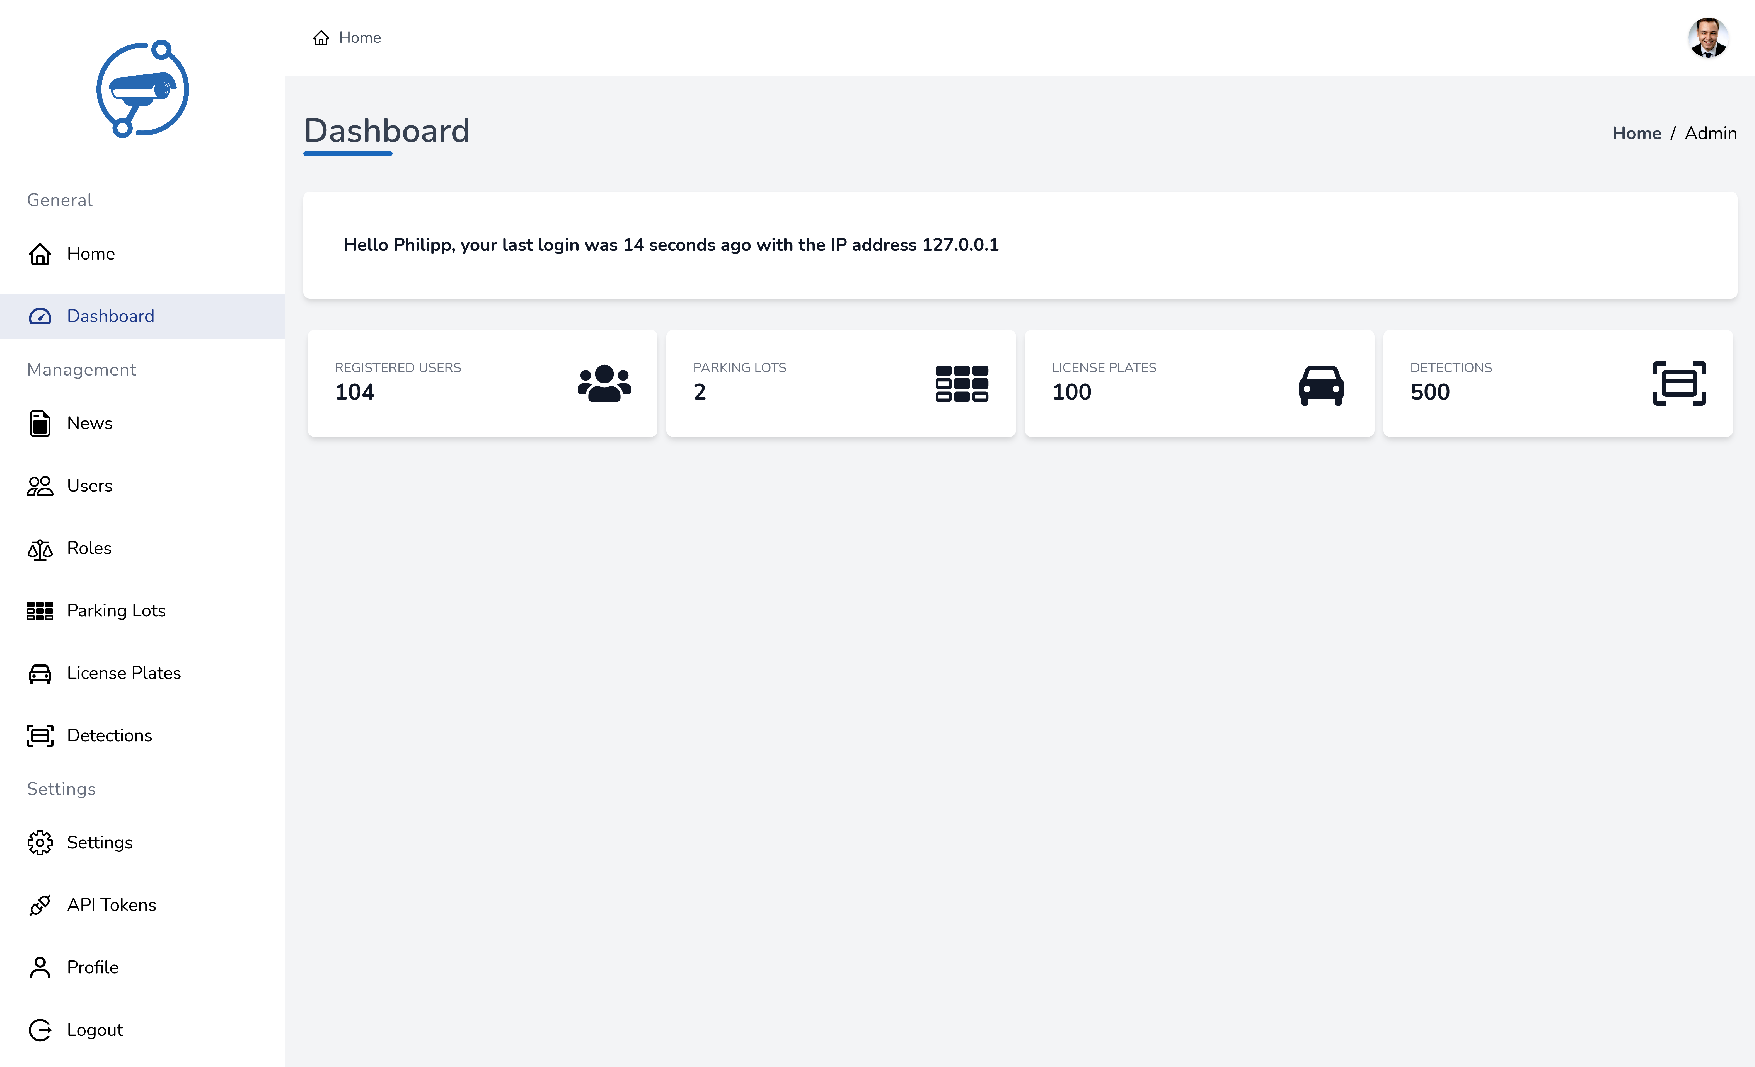
\includegraphics[width=1\linewidth]{webinterface/dashboard_site.pdf}}
  \caption{Dashboard mit Admin Layout}
\end{figure}

Im Dashboard wird das Admin Layout verwendet, somit befindet sich Links vom Page
Content nun eine Sidebar mit weiteren Links zu anderen Administrativen Seiten.\\

Um nun die Funktion besser zu verstehen wird nun auf den Code einzelner
Components genauer eingegangen.

\subsubsection{Navbar}
Die Navigationsleiste auch Navbar genannt ist ein zentrales Element der Webseite
um verschiedene Seiten anzusteuern. Dabei veränderte sich diese dynamisch, je
nachdem ob man eingeloggt ist oder ob ein bestimmtes Feature wie das
Registrieren von neuen Benutzern deaktiviert ist.

\begin{listing}[H]
  \begin{minted}{html}
    @if (!(\Request::is('admin/*') || \Request::is('admin')))
      <a class="flex title-font font-medium items-center text-gray-900 mr-8">
         <x-application-logo class="max-h-12" />
      </a>
    @if (!Auth::guest())
      <a href="{{ route('dashboard') }}">{{ __('Dashboard') }}</a>
    @endif
    @endif
  \end{minted}
  \caption{Ausschnitt 1 navigation.blade.php}
\end{listing}

Der Ausschnitt 1 regelt das Aussehen der Navigationsleiste wenn ein Benutzer
eingeloggt ist. Dabei wird kein Logo angezeigt wenn der Benutzer eine
administrative Seite öffnet, da das Logo bereits in der
Sidebar vorhanden ist. Ebenfalls wird auf nicht administrativen Seiten ein
zurück zum Dashboard Link angezeigt.

\begin{figure}[H]
  \centering
  \frame{
\includegraphics[width=1\linewidth]{webinterface/navbar_1.pdf}}
  \caption{Navbar Variante 1}
\end{figure}

\begin{figure}[H]
  \centering
  \frame{
\includegraphics[width=1\linewidth]{webinterface/navbar_3.pdf}}
  \caption{Navbar Variante 2}
\end{figure}

\begin{listing}[H]
  \begin{minted}{html}
    @if (Auth::guest())
      <div class="flex items-center">
      <a href="{{ route('login') }}">{{ __('Login') }}</a>
    @if (Route::has('register'))
      <a href="{{ route('register') }}">{{ __('Register') }}</a>
    @endif
      </div>
    @endif
  \end{minted}
  \caption{Ausschnitt 2 navigation.blade.php}
\end{listing}

Im zweiten Ausschnitt geht es um die Login/Register Links, diese werden nur
nicht eingeloggten Benutzern angezeigt. Ob der Register Link angezeigt wird ist
abhängig von den getätigten Einstellungen in den Seiten Einstellungen.

\begin{figure}[H]
  \centering
  \frame{
\includegraphics[width=1\linewidth]{webinterface/navbar_2.pdf}}
  \caption{Navbar Variante 3}
\end{figure}

\subsubsection{Content Header}
Um die Navigation zu erleichtern besitzt das Webinterface bei Seiten mit dem
\verb|admin|-Layout unter der Navigationsleiste einen Content Header. Der
Content Header setzt sich aus dem Seiten Titel und den sogenannten Breadcrumbs\footnote{engl.
für Brotkrümel, entspricht einer Navigation} zusammen. Dabei befindet sich ganz
links der aktuelle Seiten Titel, welcher ebenfalls im Browser Tab angezeigt wird
und rechts die Brotkrümelnavigation. Die Breadcrumbs geben dabei dem Benutzer an
in welcher Verzweigung er sich aktuell befindet.\\

Die Breadcrumbs werden aus der URL aufgebaut, dabei werden die einzelnen
Segmente zerlegt und in einer Liste mit Hyperlinks zusammengeführt.  

\begin{listing}[H]
  \begin{minted}{php}
    <li><a href="/" class="text-gray-700 font-bold">Home</a></li>
    <?php $link = ''; ?>
    @for ($i = 1; $i <= count(Request::segments()); $i++)
    @if (($i < count(Request::segments())) & ($i> 0))
      <?php $link .= '/' . Request::segment($i); ?>
      <li><span class="mx-2">/</span></li>
      <li><a href="<?= $link ?>" class="text-gray-700 font-bold">{{ ucwords(str_replace('-', ' ', Request::segment($i))) }}</a></li>
    @else 
      <li><span class="mx-2">/</span></li>
      <li>{{ ucwords(str_replace('-', ' ', Request::segment($i))) }}</li>
    @endif
    @endfor
  \end{minted}
  \caption{Erstellung der Breadcrumbs}
\end{listing}

\begin{figure}[H]
  \centering
  \frame{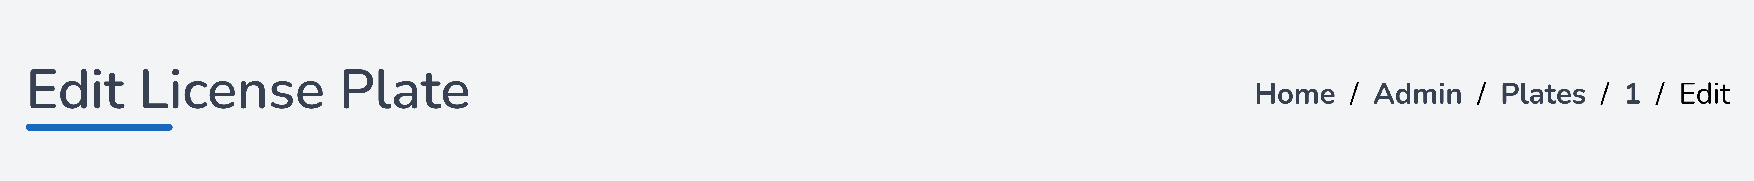
\includegraphics[width=1\linewidth]{webinterface/content_header.pdf}}
  \caption{Content Header}
\end{figure}

\subsubsection{Session Alerts}
Um einen Benutzer zu informieren, dass eine Anfrage erfolgreich ausgeführt wurde
oder ob es einen Fehler gab werden \textit{Session Alerts} verwendet.\\

Wird beispielsweise ein neues Kennzeichen im System angelegt, so wird der
Benutzer nicht nur zu der Liste aller Kennzeichen geleitet, sondern es wird in
der Session des Browsers eine Nachricht mitgespeichert.

\begin{listing}[H]
  \begin{minted}{php}
    <?php
    return redirect(route('plates.index'))->with('success', __('The license plate was successfully created!'));
  \end{minted}
  \caption{Controller mit success Nachricht}
\end{listing}

Um diese Nachricht nun anzuzeigen wurde ein Component entworfen welcher nur
angezeigt wird, wenn ein solche Session Nachricht vorhanden ist. Neben einer
\textit{success} Nachricht gibt es auch noch eine \textit{error} Nachricht,
diese wird bei fehlerhaften Angaben in einem Formular verwendet.

\begin{listing}[H]
  \begin{minted}{html}
    @if (session('success'))
    <div class="bg-green-200 px-6 py-4 mb-4 rounded-md text-lg flex items-center justify-items-stretch">
      <span class="text-green-800">{{ session('success') }}</span>
    </div>
    @endif
  \end{minted}
  \caption{Session Alert Component}
\end{listing}

\begin{figure}[H]
  \centering
  \frame{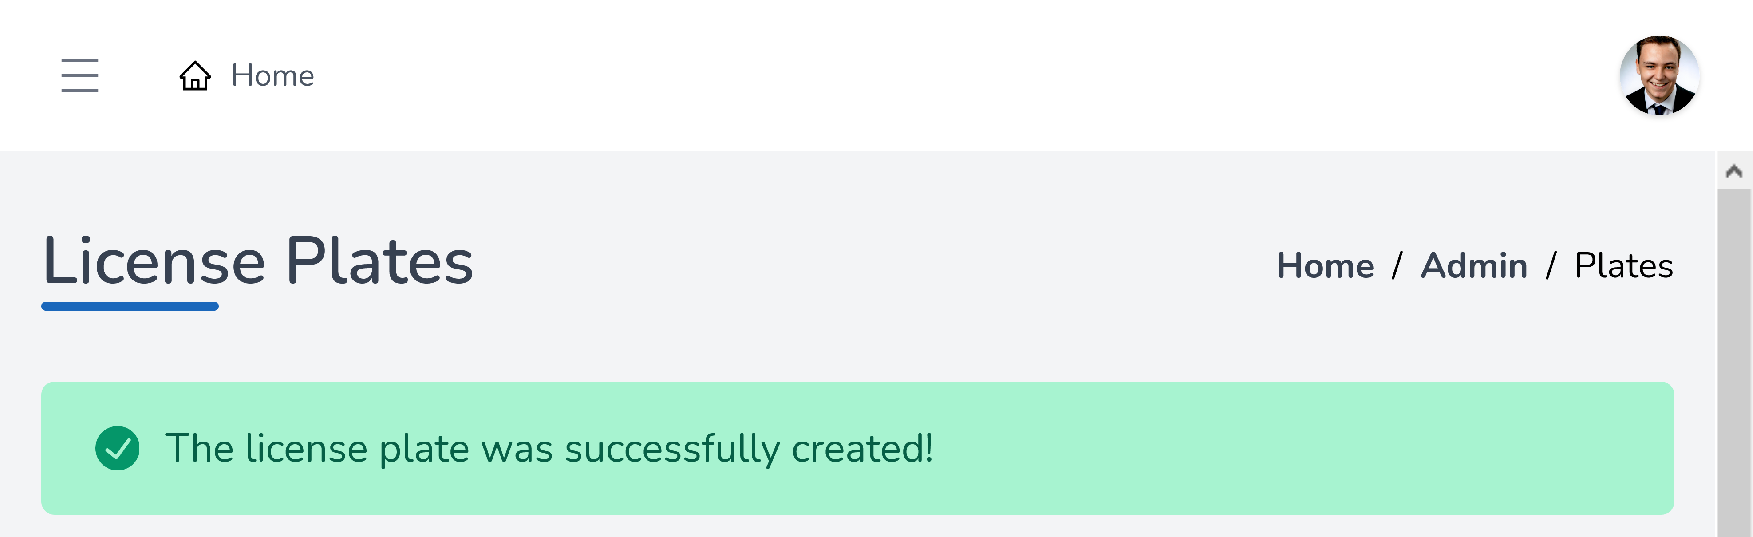
\includegraphics[width=1\linewidth]{webinterface/session_alert.pdf}}
  \caption{Success Session Alert}
\end{figure}

\subsubsection{Sidebar}
Die Sidebar ist das zentrale Element für administrative Benutzer des
Webinterfaces. Über die Sidebar sind alle wichtigen Seiten auf einen Blick zu
sehen und erreichen, dabei spielt es keine Rolle ob auf dem Smartphone oder auf
dem Desktop, denn die Sidebar wurde so implementiert, dass sie auf kleineren
Auflösungen eingeklappt wird und nur auf Wunsch mit einem das
Hamburger-Menü-Symbol\footnote{Drei waagrechte Striche ähneln einem Hamburger}
in der Navigationsleiste geöffnet, somit wird wichtiger Platz gespart.\\

Für das dynamische Verhalten der Sidebar wird \acl*{JS} verwendet. Es wird nicht
Vanilla\footnote{Bedeutet so viel wie ohne Zusätze} \acl*{JS} verwendet, sondern
AlpineJS\footnote{\url{https://github.com/alpinejs/alpine}}. Dabei folgt das
Lightweight Framework einem ähnlichen Prinzip wie TailwindCSS nur eben für
JavaScript.\\

Die Sidebar Einträge bestehen aus zwei Components, dem Sidebar Header Component
und dem Sidebar Link Component. Der Sidebar Header Component ist da um die verschiedenen Links in verschiedene
Sektionen aufzuteilen, damit die Übersichtlichkeit gewährt bleibt.

\begin{listing}[H]
  \begin{minted}{html}
    <x-sidebar-header>{{ __('General') }}</x-sidebar-header>
  \end{minted}
  \caption{Sidebar Header}
\end{listing}

Der Sidebar Link Component ist für die Links zuständig. Dieser besteht aus einem
\acs*{SVG}-Icon und dem Namen der Seite. Die Route wird dem Component über
\verb|:href| übergeben und nicht mit \verb|href|, da die URL mit einer Helper Methode
angegeben wird und ansonsten von Blade nicht compiliert wird und als
tatsächlicher Hyperlink angenommen wird.

\begin{listing}[H]
  \begin{minted}{html}
    <x-sidebar-link :href="route('home')" :active="request()->routeIs('home')">
      <span class="iconify h-6 w-6" data-icon="bx:bx-home" data-inline="false"></span>
      <span class="mx-3">{{ __('Home') }}</span>
    </x-sidebar-link>
  \end{minted}
  \caption{Sidebar Link}
\end{listing}
\begin{figure}[H]
  \centering
  \frame{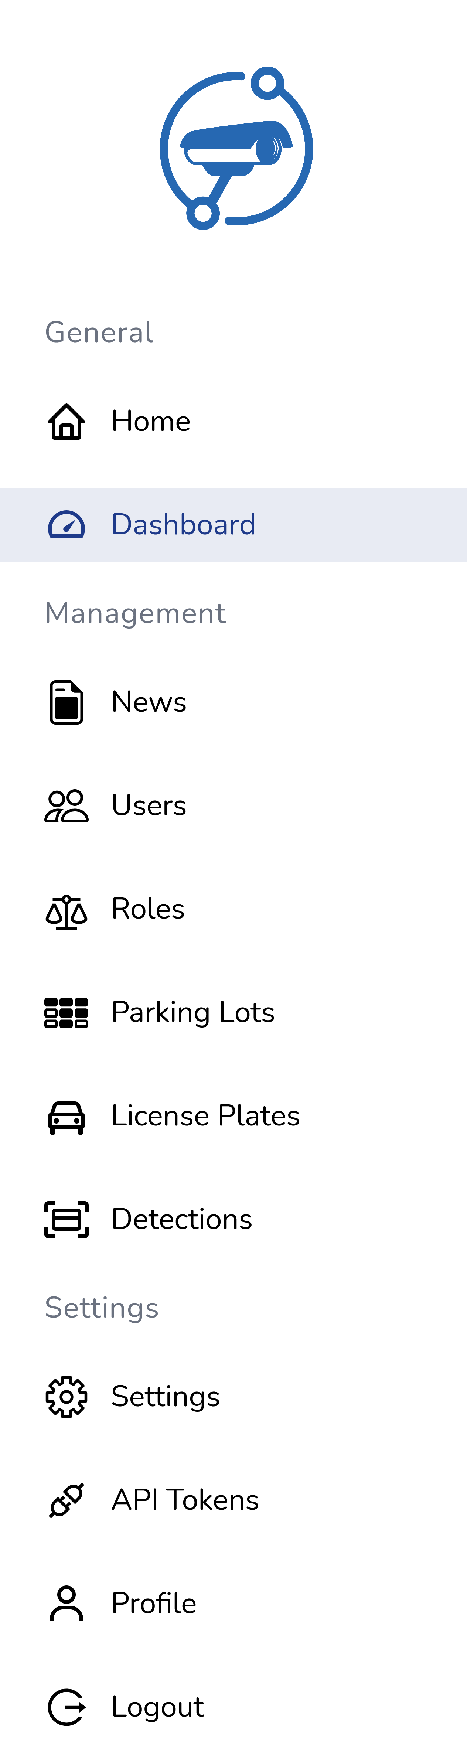
\includegraphics[width=0.35\linewidth]{webinterface/sidebar_desktop.pdf}}
  \caption{Sidebar Desktop}
\end{figure}

\subsubsection{Footer}
Der Footer ist dazu da um Informationen rund um Impressum, Datenschutzverweis,
Geschäftsbedingungen und Urheberrechtshinweis darzustellen.\\

Grundsätzlich ist besitzt der Footer des Webinterfaces auf der linken Seite
einen variablen Text der sich frei über die Seiten Einstellungen einstellen
lässt und auf der rechten Seiten Verweise auf die Datenschutzbestimmungen,
Allgemeine Geschäftsbedingungen und Impressum welche sich ebenfalls über die
Seiten Einstellungen konfigurieren lassen. Befindet sich auf diesen Seiten kein
Inhalt werden diese auch nicht im Footer angezeigt.

\begin{figure}[H]
  \centering
  \frame{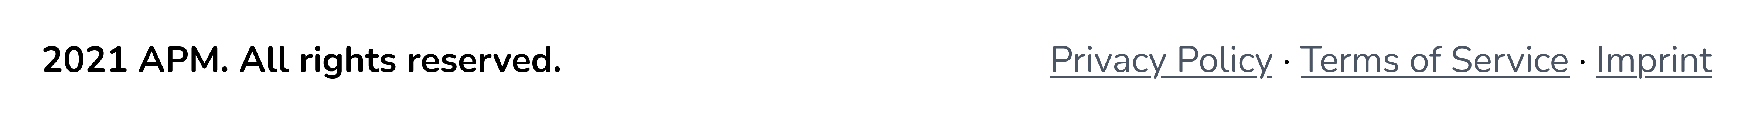
\includegraphics[width=1\linewidth]{webinterface/footer.pdf}}
  \caption{Footer}
\end{figure}

\subsection{Funktionen}
Das Webinterface besitzt eine große Anzahl an Features und
Konfigurationsmöglichkeiten. In den folgenden Seiten werden alle Funktionen
ausführlich mit deren technischen Funktion erklärt.

\subsubsection{Dashboard}
Das Dashboard ist praktisch die Startseite für eingeloggte Benutzer, als erstes
wird dem Benutzer eine Sicherheitsnachricht über den letzten Login angezeigt.
Dabei wird die Zeit seit dem letzten Login angegeben und die dabei verwendete
IP-Adresse.\\

Um diese Daten zu speichern wird im \verb|AuthenticatedSessionController| die
\verb|store| Methode ergänzt. Dabei wird nachdem sich der Benutzer erfolgreich
Authentifiziert hat die IP-Adresse und der aktuelle Zeitpunkt in die Datenbank
geschrieben.

\begin{listing}[H]
  \begin{minted}{php}
    <?php
    $user = Auth::user();
    $user->last_login_at = Carbon::now()->toDateTimeString();
    $user->last_login_ip = $request->getClientIp();
    $user->save();
  \end{minted}
  \caption{AuthenticatedSessionController.php Store Methode}
\end{listing}

\begin{figure}[H]
  \centering
  \frame{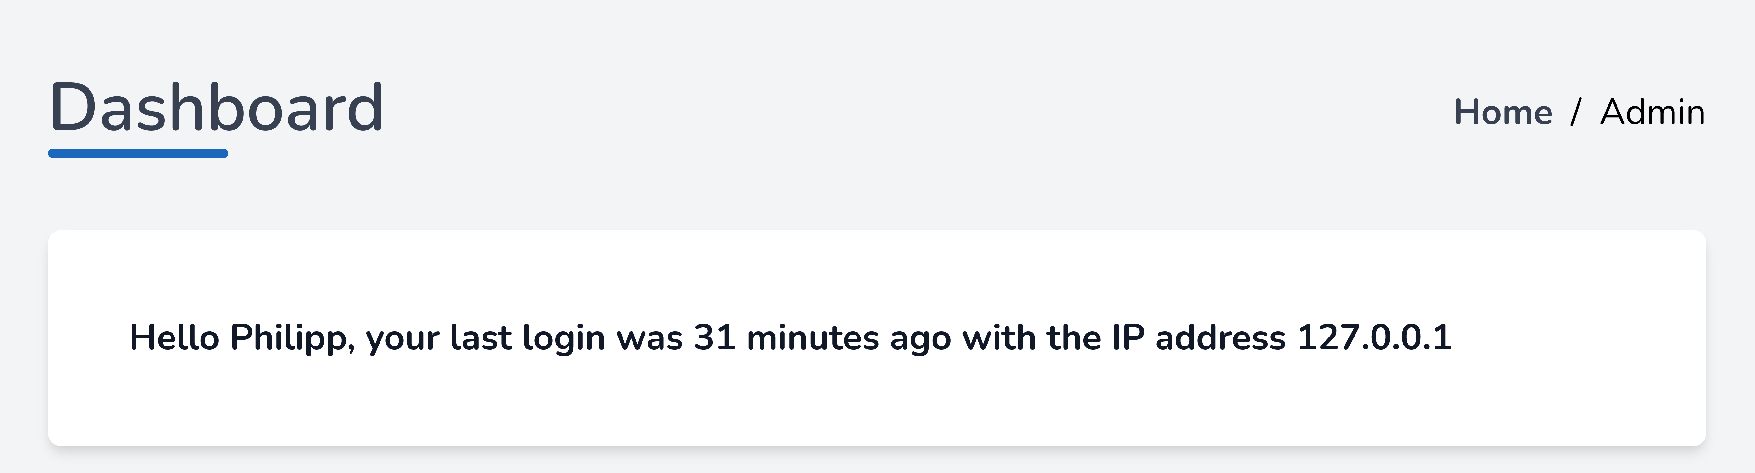
\includegraphics[width=1\linewidth]{webinterface/sicherheitsnachricht.pdf}}
  \caption{Dashboard Sicherheitsnachricht}
\end{figure}

Neben der Sicherheitsnachricht werden einige statistische Zahlen über das System
dargestellt:

\begin{itemize}
  \item Anzahl der registrierten Benutzer
  \item Anzahl der Parkplätze im System
  \item Anzahl der bekannten Kennzeichen
  \item Anzahl der erkannten Kennzeichens
\end{itemize}

\begin{figure}[H]
  \centering
  \frame{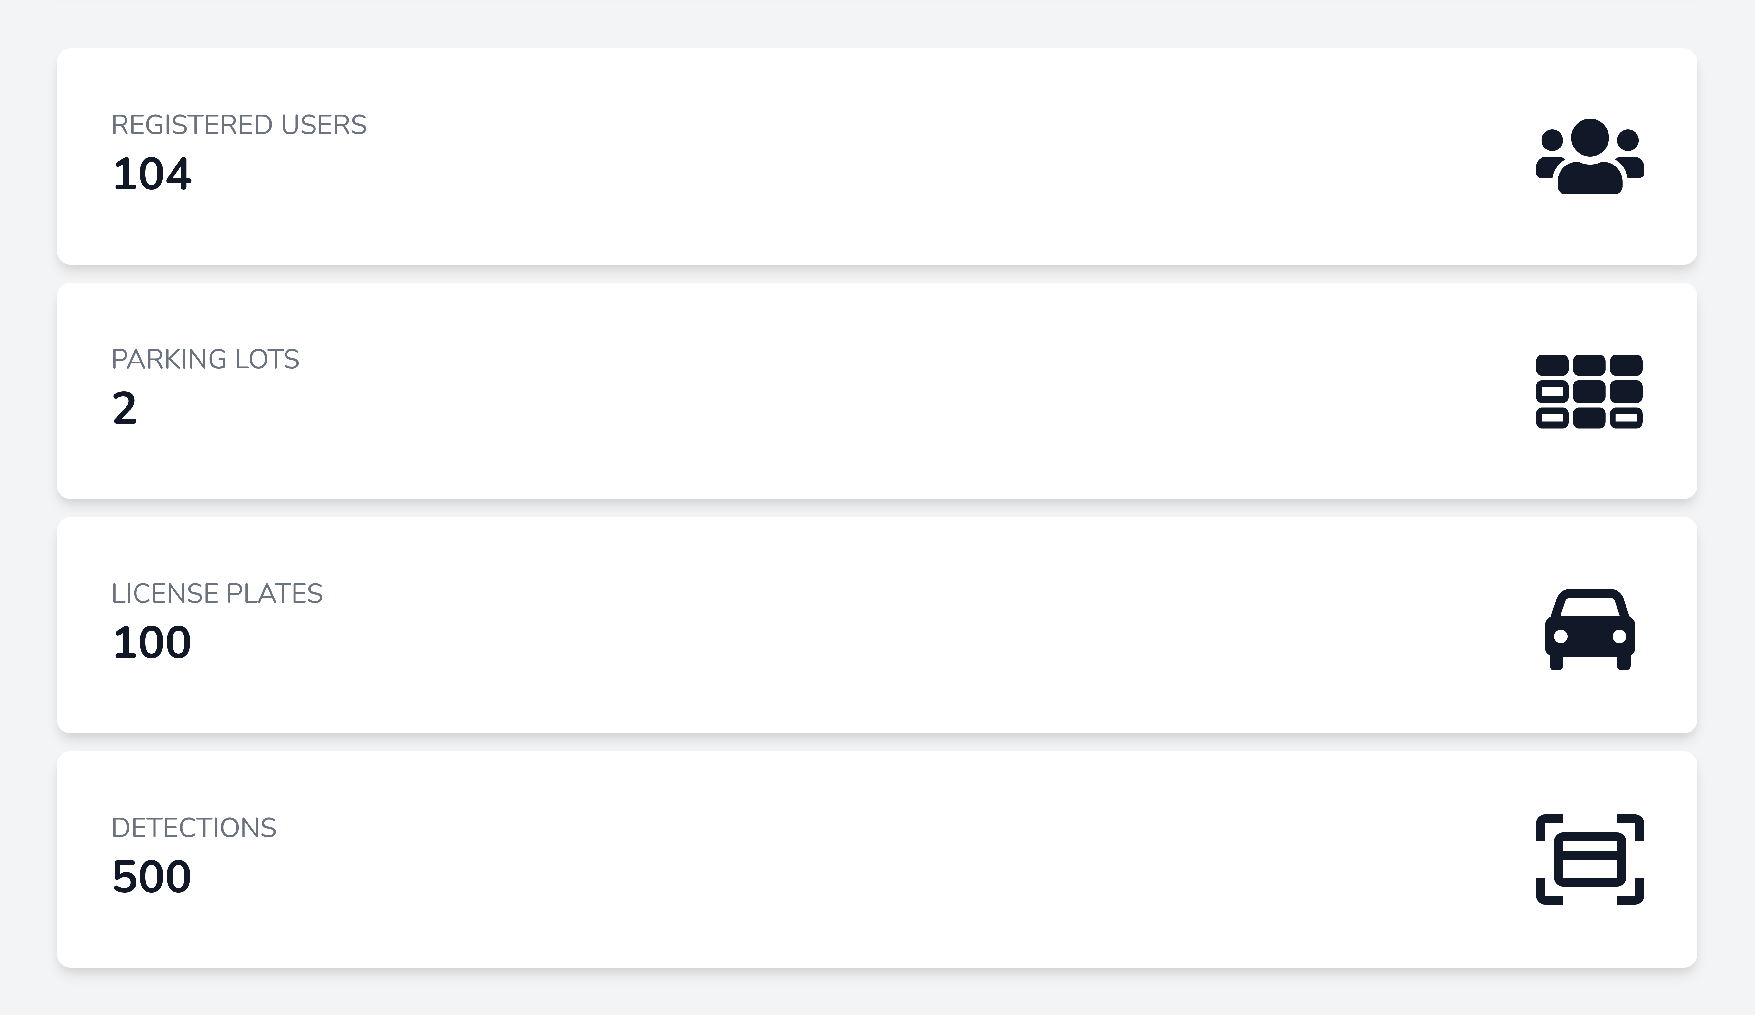
\includegraphics[width=1\linewidth]{webinterface/dashboard_stats.pdf}}
  \caption{Dashboard Statistik}
\end{figure}

\subsubsection{Benutzerverwaltung}

Die Benutzerverwaltung ist ein zentrales Steuerelement des Webinterfaces und wichtig
für die Zugriffskontrolle. Für die Benutzerverwaltung sind alle CRUD-Operationen\footnote{Grundlegende Operationen:
Create, Read, Update und Delete} verfügbar.

\begin{figure}[H]
  \centering
  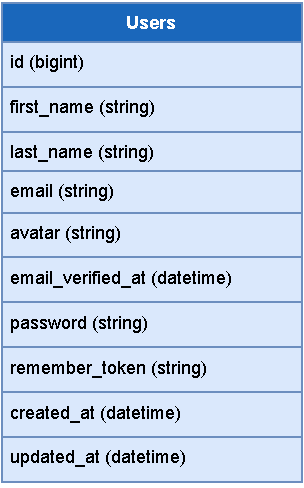
\includegraphics[width=0.3\linewidth]{webinterface/user_table.pdf}
  \caption{Benutzer ER}
\end{figure}

\paragraph{Liste aller Benutzer}\mbox{}\\

Die Startseite der Benutzerverwaltung ist eine Liste von allen Benutzern im
System. Dort sind die wichtigsten Informationen direkt abzulesen wie Name, Rolle
und Email.

\begin{figure}[H]
  \centering
  \frame{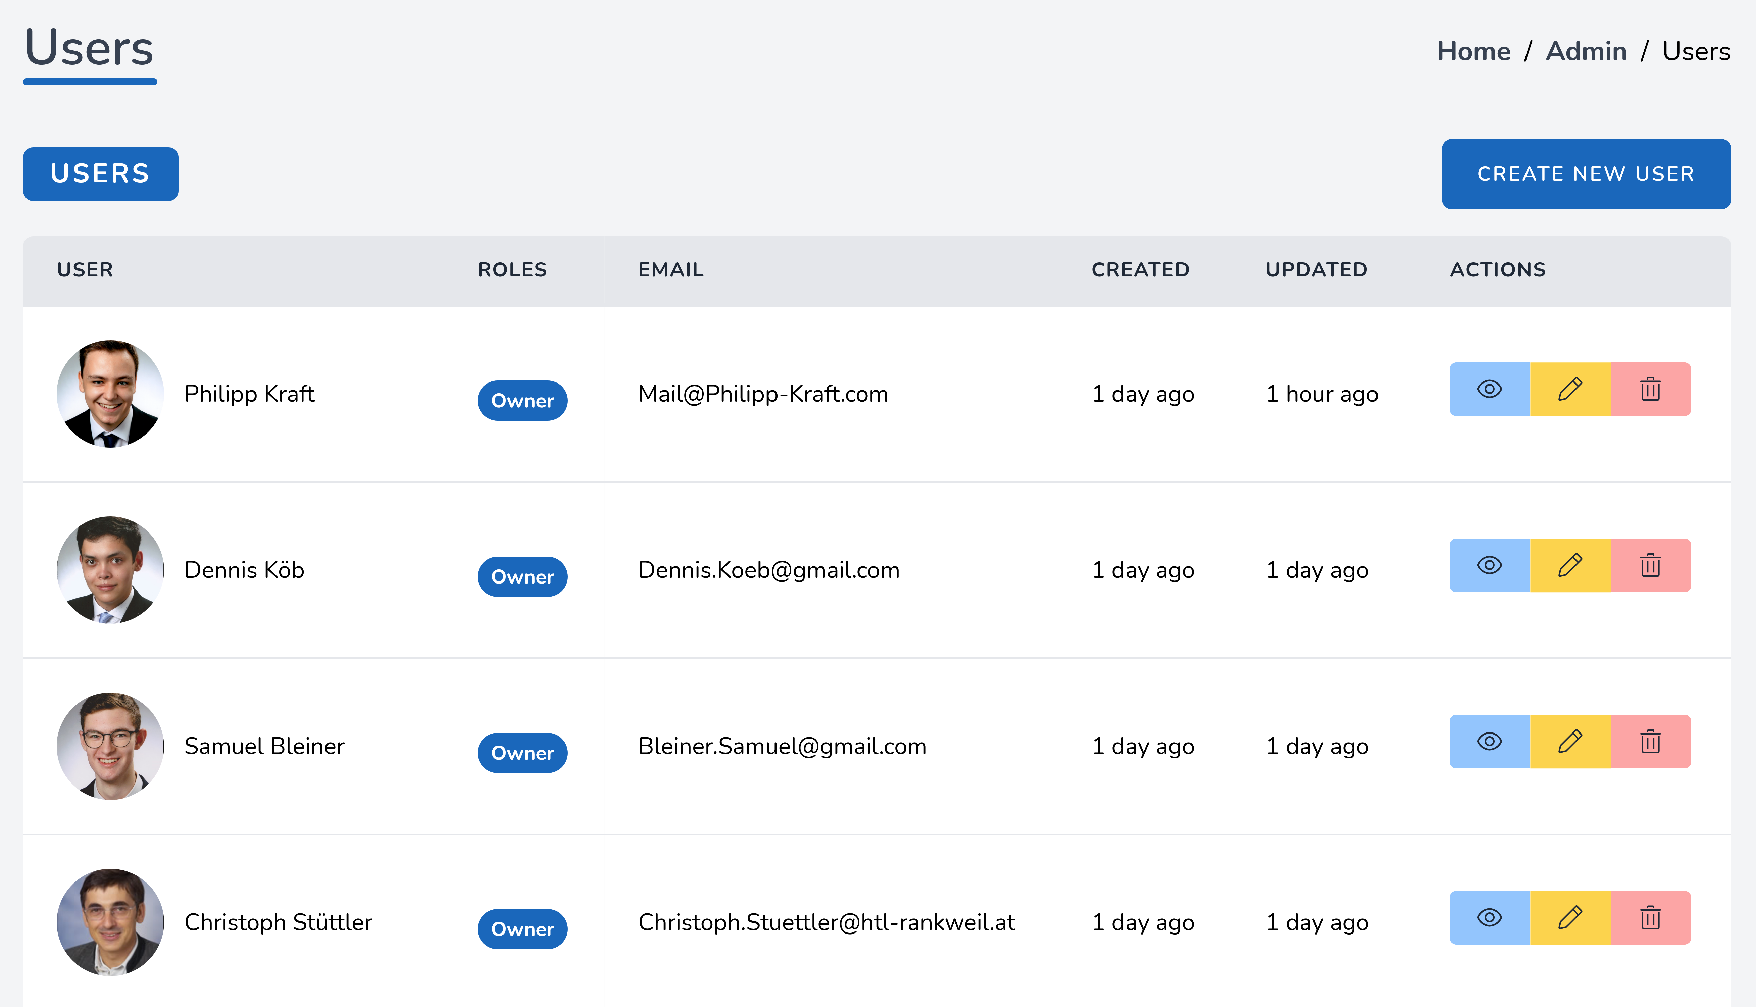
\includegraphics[width=1\linewidth]{webinterface/users_index.pdf}}
  \caption{Liste aller Benutzer}
\end{figure}

\paragraph{Benutzer erstellen/editieren}\mbox{}\\

Neue Benutzer können mit dem Button rechts oben über \verb|Create new user| angelegt
werden. Einzelne Benutzer besitzen drei mögliche Aktionen in der letzten Spalte,
dabei gibt es Betrachten (Blau), Editieren (Gelb) und Löschen (Rot). Es können
folgende Informationen eines Benutzers konfiguriert werden:

\begin{itemize}
  \item Profilbild
  \item Vorname
  \item Nachname
  \item Email
  \item Passwort
  \item Rollen
\end{itemize}

\begin{figure}[H]
  \centering
  \frame{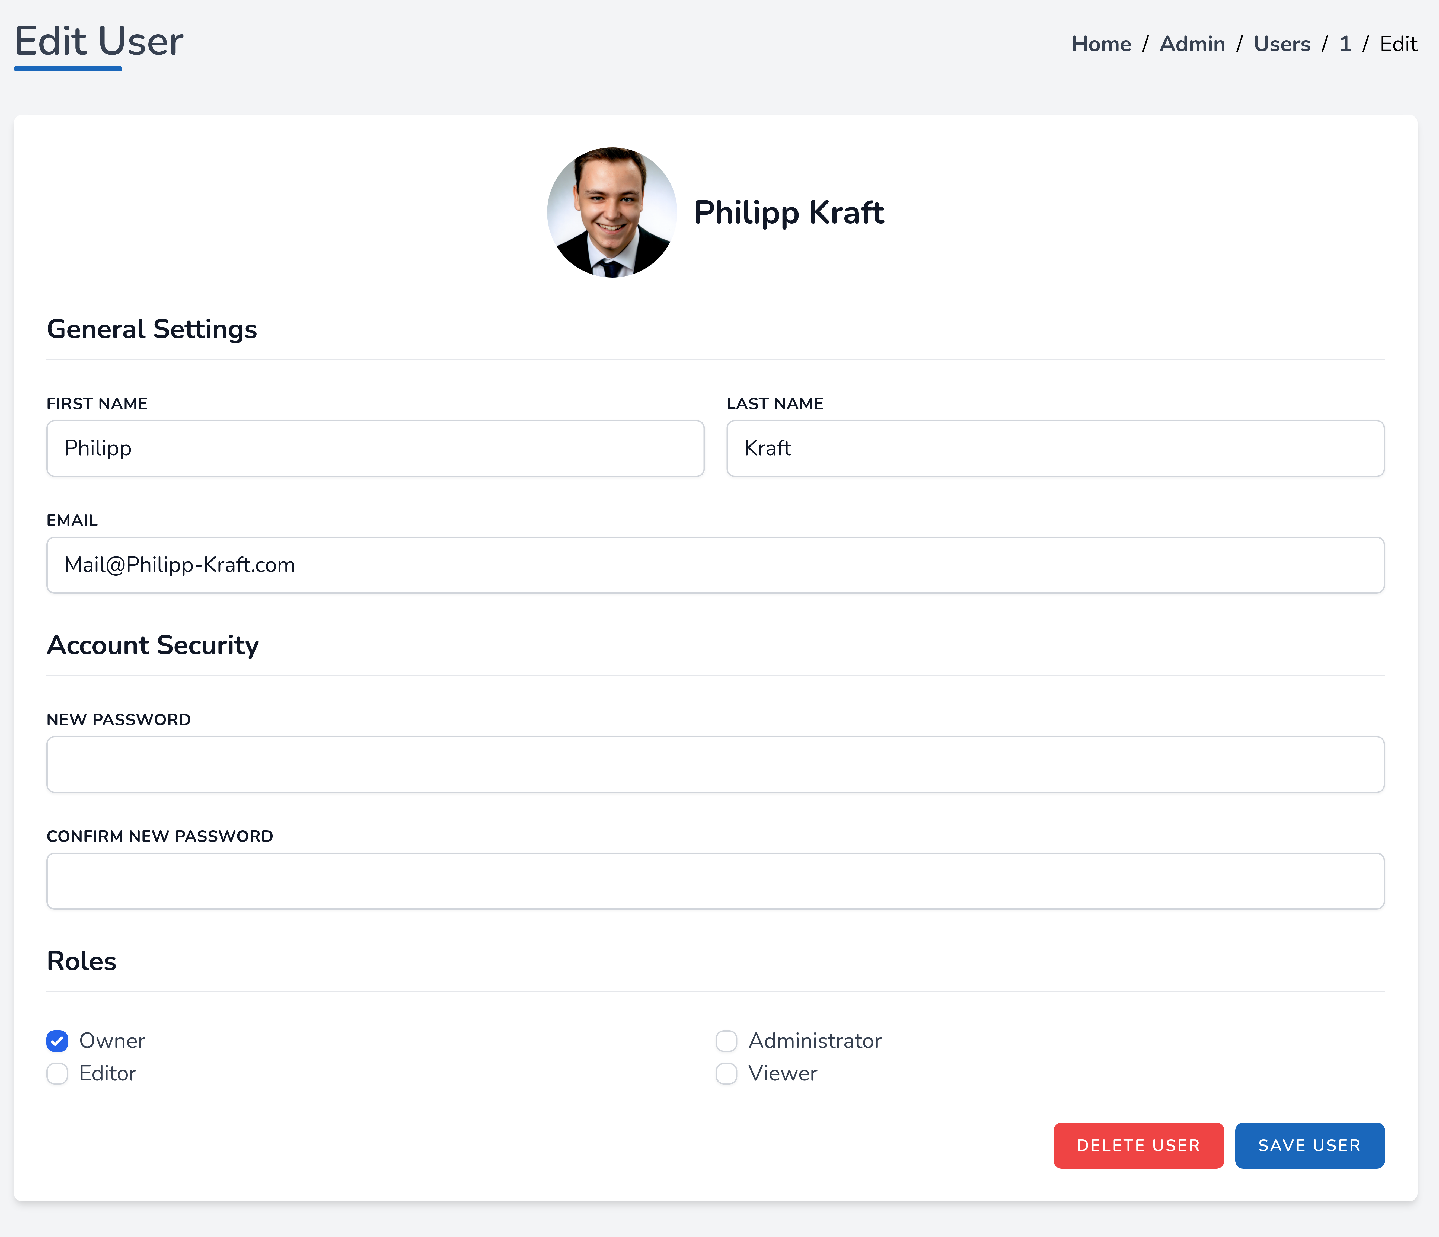
\includegraphics[width=1\linewidth]{webinterface/edit_user.pdf}}
  \caption{Benutzer editieren}
\end{figure}

\paragraph{Profilbilder}\mbox{}\\
Jeder Benutzer hat die Möglichkeit ein Profilbild zu besitzen und dies wird
überall verwendet wo ein Benutzer erwähnt wird.\\

Um ein Bild hochzuladen muss beim editieren/erstellen auf das Profilbild bzw.
auf das Standardprofilbild geklickt werden, es öffnet sich nun ein Upload-Dialog
des Betriebsystems und erlaubt es ein Bild auszuwählen.

\begin{listing}[H]
  \begin{minted}{html}
    <div class="flex justify-center items-center mt-6">
    <label for="avatar">
      <input type="file" name="avatar" id="avatar" style="display:none;" />
      <img class="w-24 h-24 object-cover rounded-full" alt="User avatar"
        src="{{ asset('/uploads/avatars/default.png') }}" />
    </label>
    </div>
  \end{minted}
  \caption{Profilbild Upload}
\end{listing}

Bevor das Bild nun auf dem Server gespeichert wird ist es notwendig es mit der
PHP Image Library
\textbf{Intervention}\footnote{\url{http://image.intervention.io/}} das Bild auf
die passende Größe zu skalieren. Nach diesem Schritt wird das Bild unter dem
Pfad \verb|/uploads/avatars/| mit einem zufälligem Namen abgespeichert und mit
dem Benutzer assoziiert.

\begin{listing}[H]
  \begin{minted}{php}
    <?php
    if ($request->hasFile('avatar')) {
      $avatar = $request->file('avatar');
      $filename = time() . '.' . $avatar->getClientOriginalExtension();

      Image::make($avatar)->resize(600, 600, function ($constraint) {
        $constraint->aspectRatio();
      })->save(public_path('/uploads/avatars/' . $filename));

      $user->avatar = $filename;
    }
  \end{minted}
  \caption{UserController.php Profilbild Upload}
\end{listing}

\subsubsection{Rollen- und Rechteverwaltung}
Die Rollen- und Rechteverwaltung ist eng mit der Benutzerverwaltung verbunden.
Dabei ist das System so aufgebaut, dass es verschiedene Rechte für bestimmte
Anfragen gibt (z.B. Benutzer editieren), diese Vielzahl an Rechten können
verschiedenen Gruppen zugewiesen werden. Schlussendlich kann man diese Gruppen
einzelnen Benutzern zuweisen.\\

Es gibt nun drei relevante Modelle (\verb|User|, \verb|Role| und \verb|Permission|), dabei
besteht zwischen dem User und dem Role Model eine m zu n Beziehung. Ebenfalls
besteht zwischen dem Role Model und dem Permission Model eine m zu n Beziehung.

\begin{figure}[H]
  \centering
  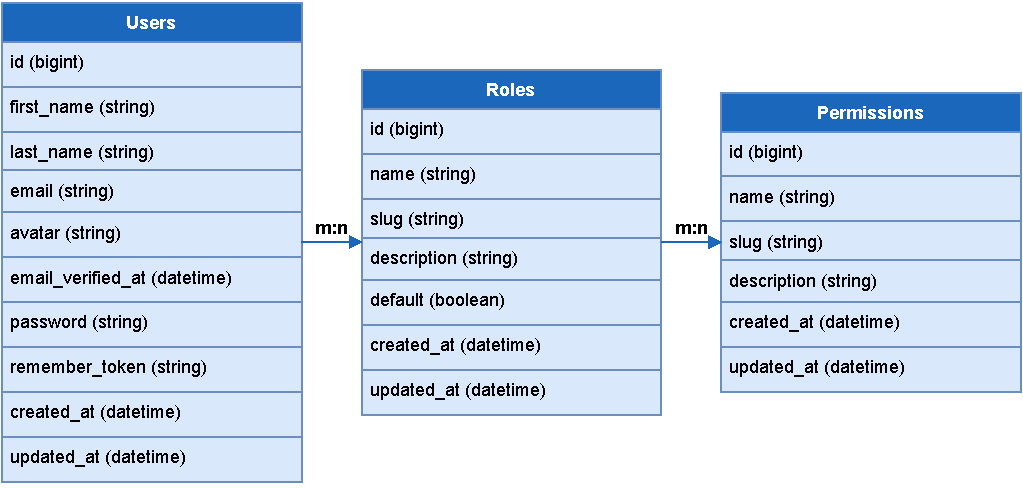
\includegraphics[width=1\linewidth]{webinterface/er_roles_permission.pdf}
  \caption{Benutzer, Rollen und Rechte ER}
\end{figure}

\paragraph{Liste der verfügbaren Rechte}\mbox{}\\

Die Rechte von einzelnen Funktionen sind ähnlich aufgebaut:

\begin{itemize}
  \item \textbf{Index <Model>:} Liste aller einzelnen Elemente der Model
  \item \textbf{Create <Model>:} Formular für das erstellen eines neuen
  Elements der Model
  \item \textbf{Store <Model>:} Neues Element der Model in die Datenbank speichern
  \item \textbf{Show <Model>:} Einzelnes Element der Model anzeigen
  \item \textbf{Edit <Model>:} Formular für das editieren eines Elements der
  Model
  \item \textbf{Update <Model>:} Vorhandenes Element der Model in der
  Datenbank aktualisieren
  \item \textbf{Destroy <Model>:} Element der Model aus der Datenbank löschen
\end{itemize}

Das Webinterface besitzt 43 verschiedene Rechte.

\begin{longtable}[c]{@{}lll@{}}
  \toprule
  \textbf{Name}         & \textbf{Slug}         & \textbf{Beschreibung}              \\* \midrule
  \endfirsthead
  %
  \endhead
  %
  \bottomrule
  \endfoot
  %
  \endlastfoot
  %
  Index Post            & index-post            & Liste aller Neuigkeit anzeigen     \\
  Create Post           & create-post           & Neuigkeit erstellen                \\
  Store Post            & store-post            & Neuigkeit speichern                \\
  Show Post             & show-post             & Neuigkeit anzeigen                 \\
  Edit Post             & edit-post             & Neuigkeit editieren                \\
  Update Post           & update-post           & Neuigkeit aktualisieren            \\
  Destroy Post          & destroy-post          & Neuigkeit löschen                  \\
  Index User            & index-user            & Liste aller Benutzer anzeigen      \\
  Create User           & create-user           & Benutzer erstellen                 \\
  Store User            & store-user            & Benutzer speichern                 \\
  Show User             & show-user             & Benutzer anzeigen                  \\
  Edit User             & edit-user             & Benutzer editieren                 \\
  Update User           & update-user           & Benutzer aktualisieren             \\
  Destroy User          & destroy-user          & Benutzer löschen                   \\
  Index License Plate   & index-license-plate   & Liste aller Kennzeichen anzeigen   \\
  Create License Plate  & create-license-plate  & Kennzeichen erstellen              \\
  Store License Plate   & store-license-plate   & Kennzeichen speichern              \\
  Show License Plate    & show-license-plate    & Kennzeichen anzeigen               \\
  Edit License Plate    & edit-license-plate    & Kennzeichen editieren              \\
  Update License Plate  & update-license-plate  & Kennzeichen aktualisieren          \\
  Destroy License Plate & destroy-license-plate & Kennzeichen löschen                \\
  Index Detection       & index-detection       & Liste aller Erkennungen anzeigen   \\
  Index Parking Lot     & index-parking-lot     & Liste aller Parkplätze anzeigen    \\
  Create Parking Lot    & create-parking-lot    & Parkplätze erstellen               \\
  Store Parking Lot     & store-parking-lot     & Parkplätze speichern               \\
  Edit Parking Lot      & edit-parking-lot      & Parkplätze editieren               \\
  Update Parking Lot    & update-parking-lot    & Parkplätze aktualisieren           \\
  Destroy Parking Lot   & destroy-parking-lot   & Parkplätze löschen                 \\
  Store Parking Spot    & store-parking-lot     & Parkplätze speichern               \\
  Destroy Parking Spot  & destroy-parking-spot  & Parkplätze löschen                 \\
  Index Role            & index-role            & Liste aller Rollen anzeigen        \\
  Create Role           & create-role           & Rolle erstellen                    \\
  Store Role            & store-role            & Rolle speichern                    \\
  Show Role             & show-role             & Rolle anzeigen                     \\
  Edit Role             & edit-role             & Rolle editieren                    \\
  Update Role           & update-role           & Rolle aktualisieren                \\
  Destroy Role          & destroy-role          & Rolle löschen                      \\
  Index Setting         & index-setting         & Liste aller Einstellungen anzeigen \\
  Update Setting        & update-setting        & Einstellungen aktualisieren        \\
  Index Token           & index-token           & Liste aller API Schlüssel anzeigen \\
  Store Token           & store-token           & API Token speichern                \\
  Destroy Token         & destroy-token         & API Token löschen                  \\* \bottomrule
  \caption{Verfügbare Rechte}
\end{longtable}

\paragraph{Vergabe von Rechten und Rollen mit Slugs}\mbox{}\\
Da es bei der großen Anzahl von verschiedenen Rechte kompliziert wäre die Rechte
und Rollen mit einer ID zu vergeben wird ein Slug\footnote{Benutzerfreundlicher
Name} verwendet.

\begin{listing}[H]
  \begin{minted}{php}
    <?php
    public function givePermissionBySlug($slugs)
    {
      if (!isset($slugs))
        return;

      foreach ($slugs as $slug) {
        $permission = Permission::where('slug', $slug)->first();
        $this->permissions()->attach($permission);
      }
    }
  \end{minted}
  \caption{Permission Vergabe Methode}
\end{listing}

Mit der \verb|givePermissionBySlug| Methode ist es nun möglich Rollen eine
Vielzahl von Rechten zuzuteilen, dabei muss nur ein Array mit den Slugs der
einzelnen Rechte übergeben werden.\\

Im Codeausschnitt~\ref{lst:roleseeder} vom RoleSeeder wird eine neue Rolle mit
dem Namen \textbf{Administrator} und dem Slug \textbf{admin} erstellt,
gleichzeitig werden einige Rechte dieser Gruppe zugeteilt.

\begin{listing}[H]
  \begin{minted}{php}
    <?php
    Role::create(['name' => 'Administrator', 'slug' => 'admin'])
    ->givePermissionBySlug([
        'index-user', 'create-user', 'store-user', 'show-user', 'edit-user'
    ]);
  \end{minted}
  \caption{Rolle erstellen und Rechte zuweisen}
  \label{lst:roleseeder}
\end{listing}

Eine ähnliche Methode wird verwendet um einem Benutzer eine oder mehrere Rollen
zuzuweisen.

\paragraph{Authentisierung}\mbox{}\\
Für das Überprüfen ob ein Benutzer die korrekten Rechte besitzt werden Laravel
Policies verwendet. Es wird für jedes Modell eine Policy erstellt und für jedes
Recht eine Methode. Diese Methoden werden nun innerhalb eines Controllers
aufgerufen, liefert die Methode \verb|true| wird die Anfrage fortgesetzt,
liefert die Methode \verb|false| erhält der Benutzer einen 403 Forbidden HTTP Error.

\begin{listing}[H]
  \begin{minted}{php}
    <?php
    public function index(User $user)
    {
      $permission = Permission::where('slug', 'index-user')->first();
      return $user->hasRole($permission->roles);
    }
  \end{minted}
  \caption{UserPolicy Index}
\end{listing}

\begin{listing}[H]
  \begin{minted}{php}
    <?php
    public function index()
    {
        $this->authorize('index', User::class);
        ...
    }
  \end{minted}
  \caption{UserController Index}
\end{listing}

\paragraph{Rolle erstellen}\mbox{}\\
Eine neue Rolle kann über \verb|Roles| $\blacktriangleright$ 
\verb|Create new role| erstellt werden. Dabei können
folgende Informationen konfiguriert werden:

\begin{itemize}
  \item Rollenname
  \item Slug
  \item Beschreibung
  \item Rechte
  \item Standardrolle
\end{itemize}

Die gewünschten Rechte werden mithilfe von Checkboxen ausgewählt. Die
zusätzliche Option Standardrolle erlaubt es diese Rolle automatisch neue
registrierten Benutzern zuzuweisen.

\begin{figure}[H]
  \centering
  \frame{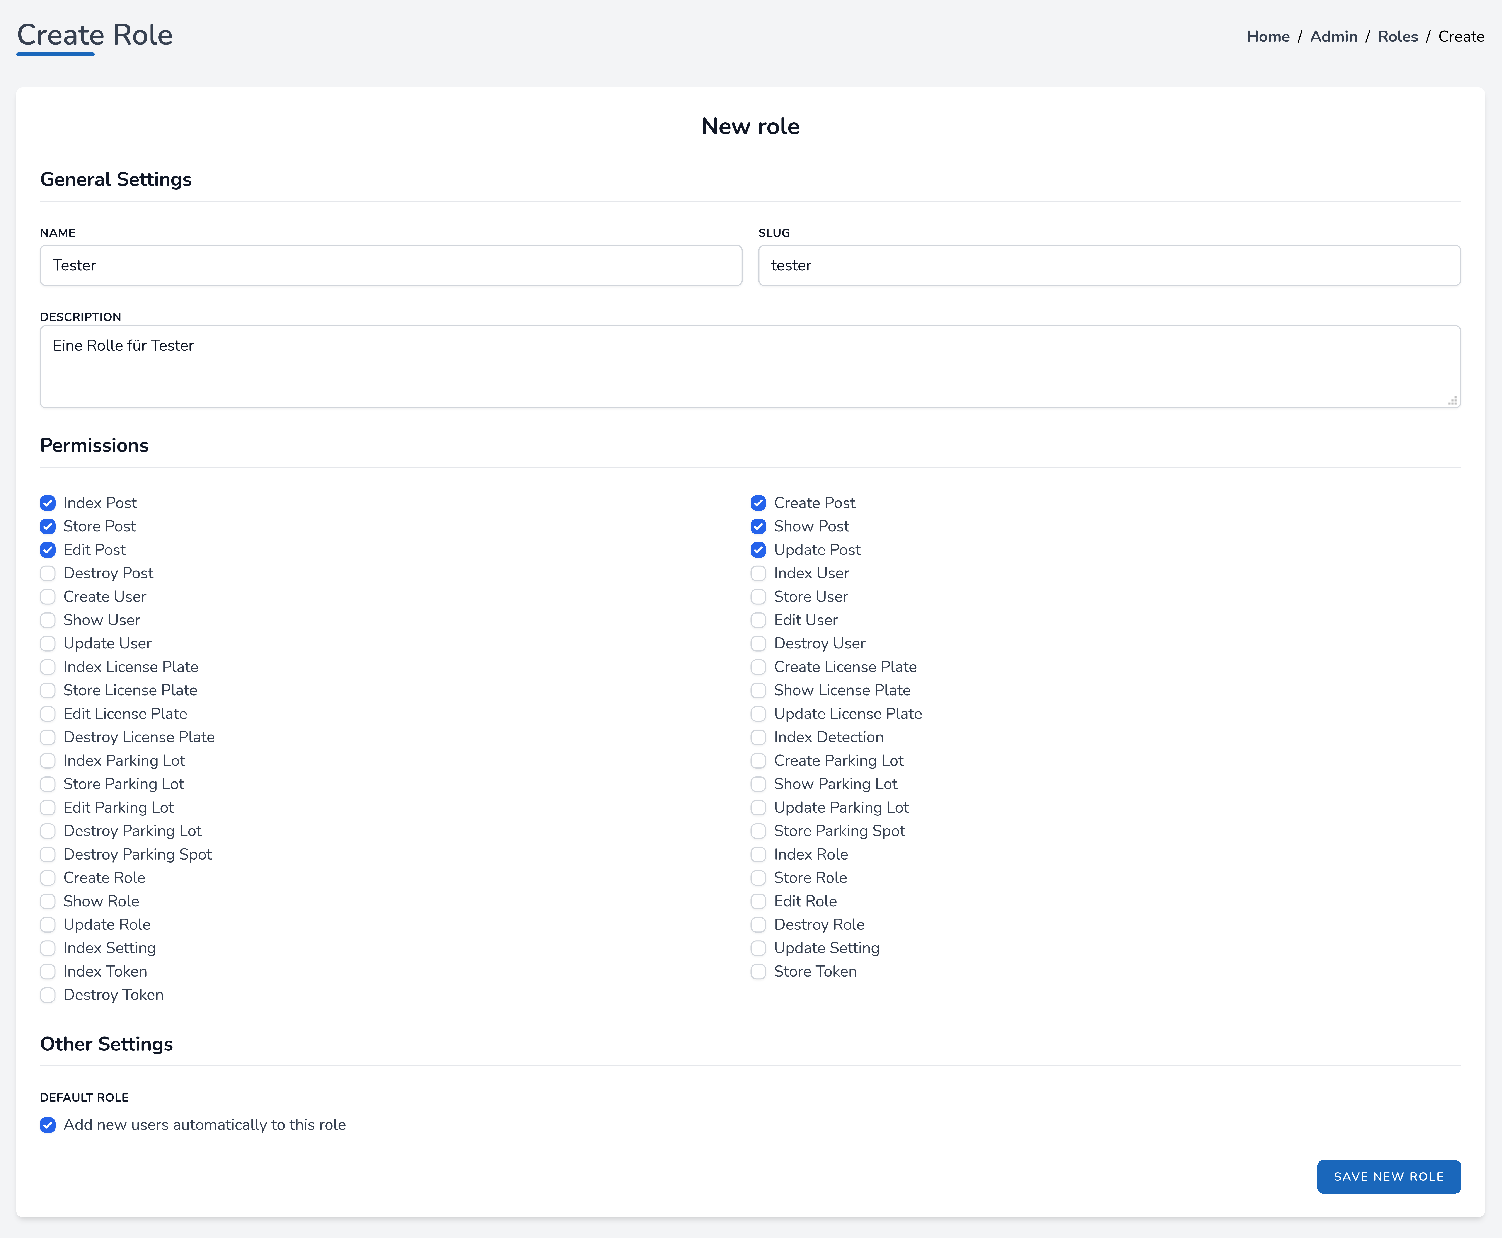
\includegraphics[width=1\linewidth]{webinterface/role_create.pdf}}
  \caption{Benutzer erstellen}
\end{figure}


\subsubsection{Neuigkeiten}
Das Neuigkeiten Feature ist eine Möglichkeit um Besucher des Webinterfaces
rasch über eine wichtige Neuigkeiten zu informieren. Dabei ist das System ähnlich
wie ein Blog aufgebaut und zeigt die einzelnen News auf der Startseite der
Webseite an. Es sind alle CRUD-Operationen verfügbar.

\begin{figure}[H]
  \centering
  \frame{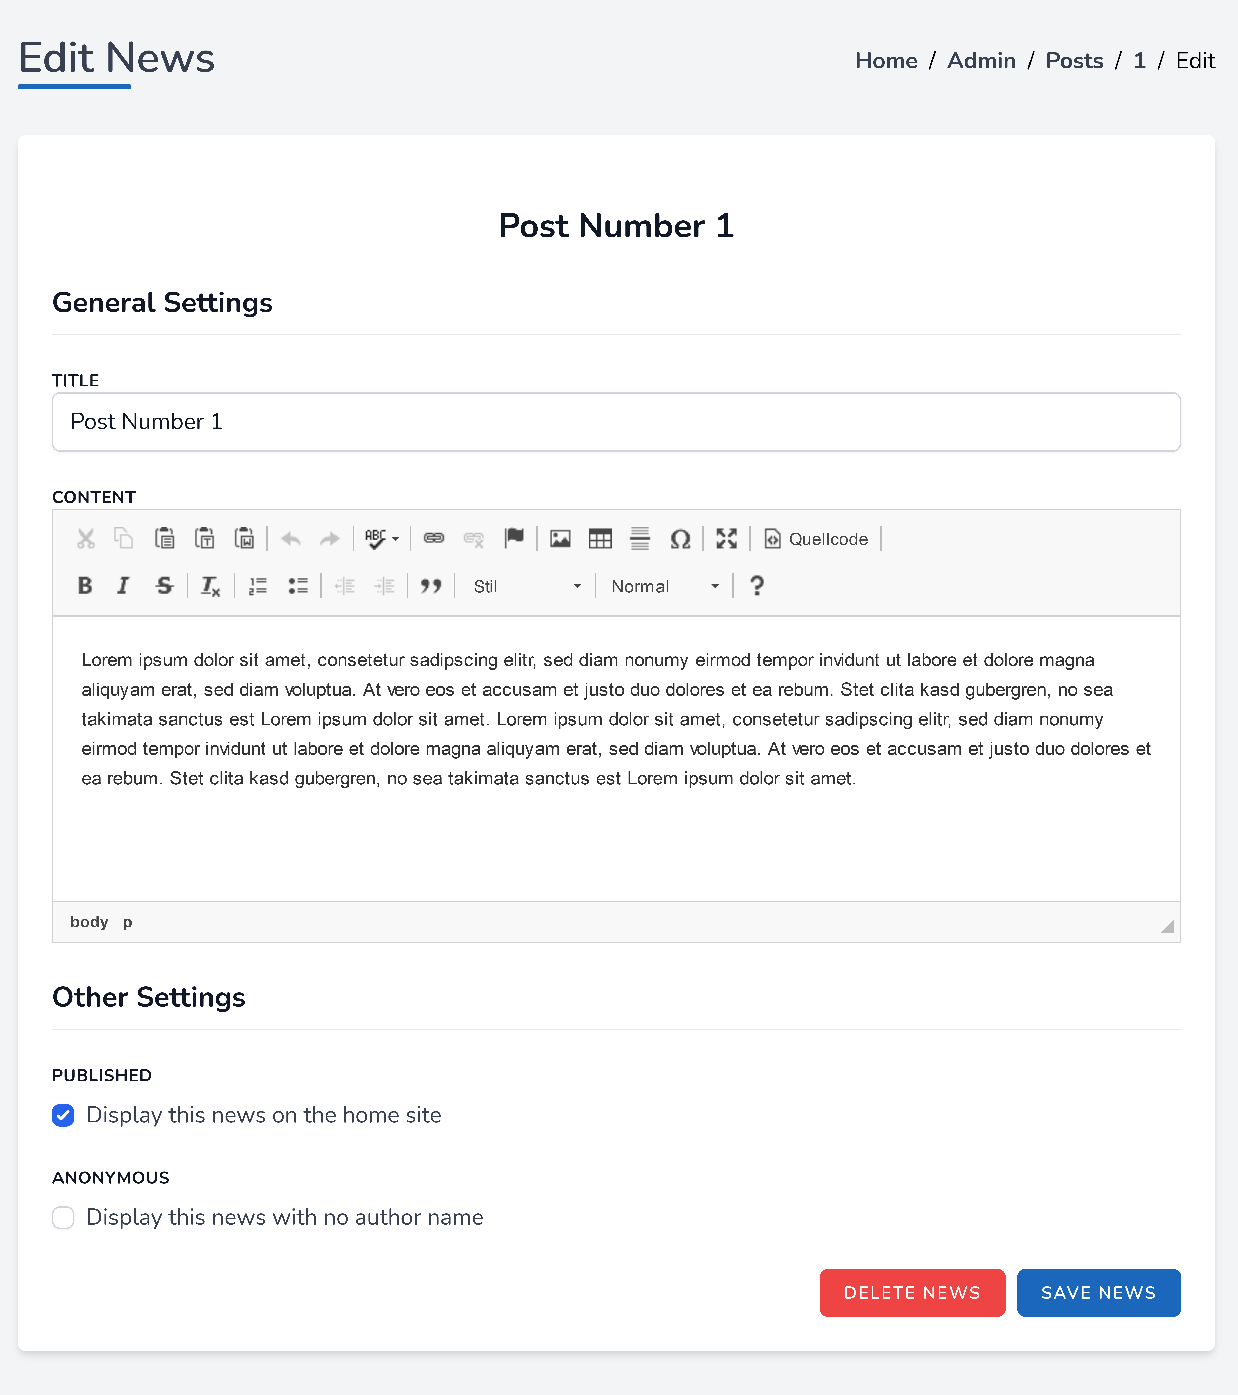
\includegraphics[width=1\linewidth]{webinterface/edit_news.pdf}}
  \caption{Neuigkeit editieren}
\end{figure}

Neben dem Titel und Inhalt gibt es noch zwei besondere Einstellungen:

\begin{itemize}
  \item \textbf{Published}\\
  Um eine Neuigkeit auf der Startseite für Besucher anzuzeigen muss diese
  Einstellung aktiviert sein. 
  \item \textbf{Anonymous}\\
  Ist es nicht erwünscht, dass der Name und das Profilbild des Autors auf der
  Startseite angezeigt wird, kann dies mit dieser Option deaktiviert werden.
\end{itemize}

Für das editieren des Inhalts wird der Quelloffene \acs*{WYSIWYG}-HTML-Editor
CKEditor 5\footnote{\url{https://ckeditor.com}} verwendet.\\

Die Startseite besitzt einen modifizierten Content Header mit dem akutellen
Datum und Uhrzeit.

\begin{figure}[H]
  \centering
  \frame{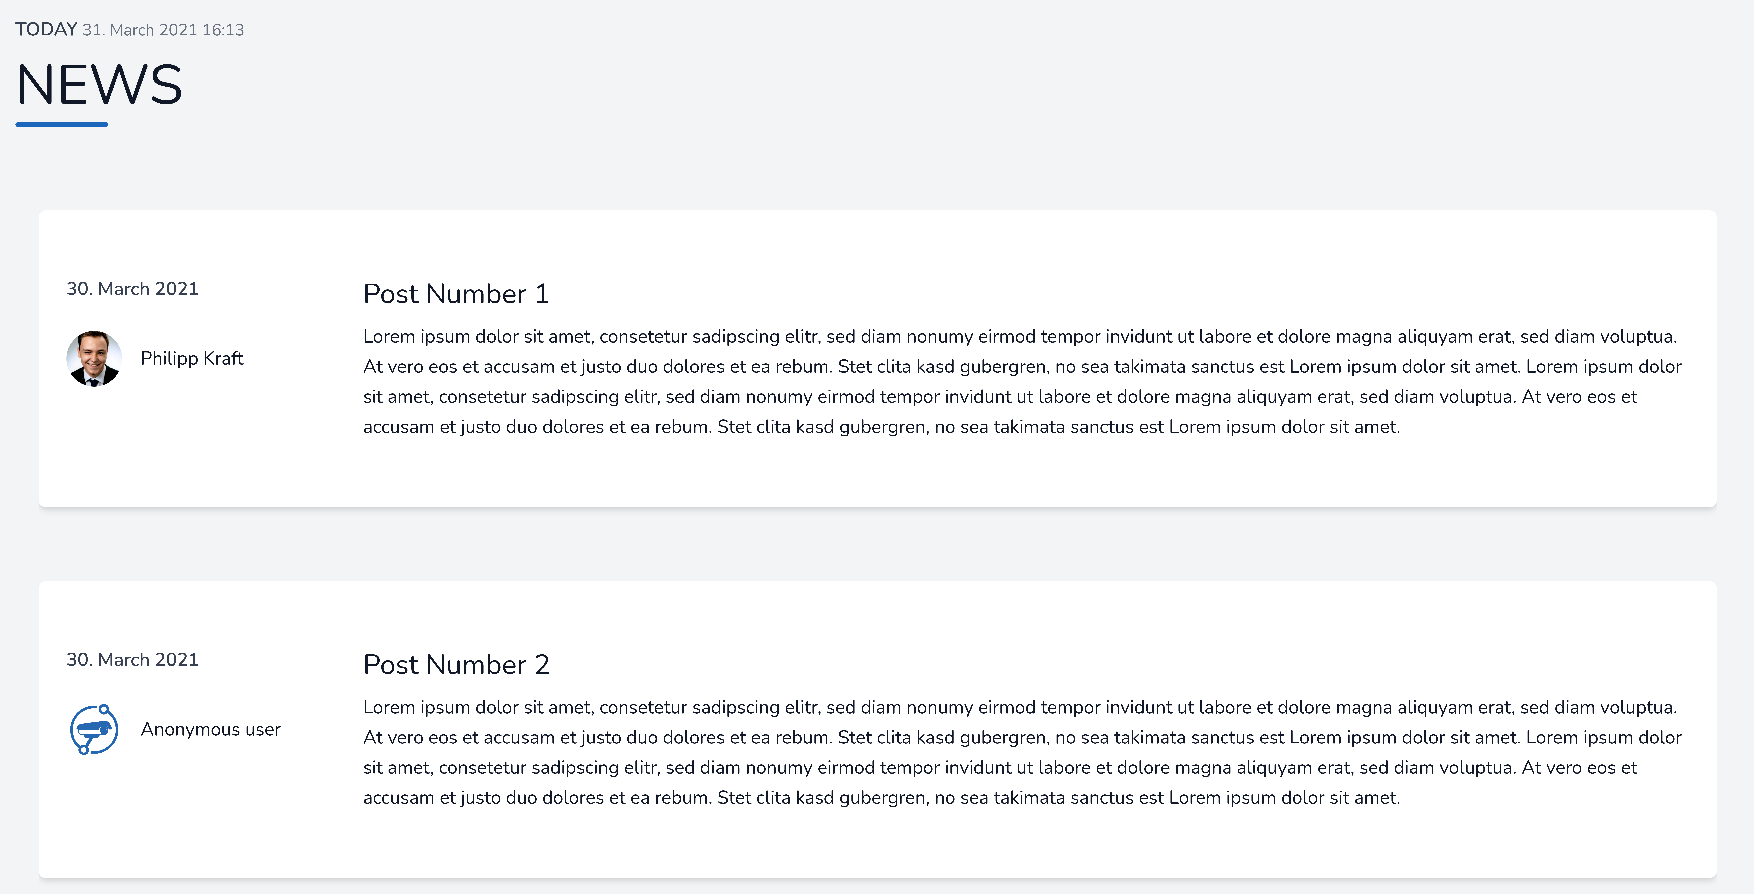
\includegraphics[width=1\linewidth]{webinterface/home.pdf}}
  \caption{Home Neuigkeiten}
\end{figure}

\subsubsection{Parkplatzverwaltung}
Ein Benutzer kann beliebig viele Parkplätze im Webinterface anlegen, ein
Parkplatz besteht dabei aus einem Namen und einer Beschreibung, ein Parkplatz
kann ebenfalls ein Bild hinzugefügt werden ähnlich wie bei den Benutzern. In der
Abbildung~\ref{fig:parking_lot_er} ist zu erkennen, dass ein Parkplatz eine 1:n
Beziehung zu den Parklücken (Parking Spots), sowie zu den Erkennungen
(Detections). 

\begin{figure}[H]
  \centering
  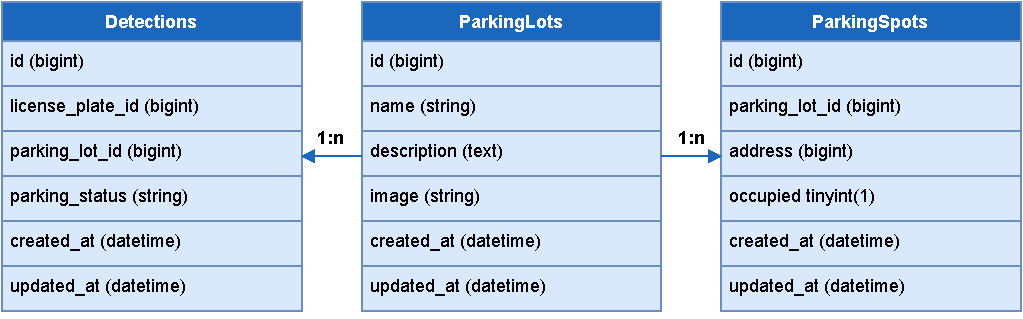
\includegraphics[width=1\linewidth]{webinterface/parking_lot_er.pdf}
  \caption{Parking Lots, Parking Spots und Detections ER}
  \label{fig:parking_lot_er}
\end{figure}

\begin{figure}[H]
  \centering
  \frame{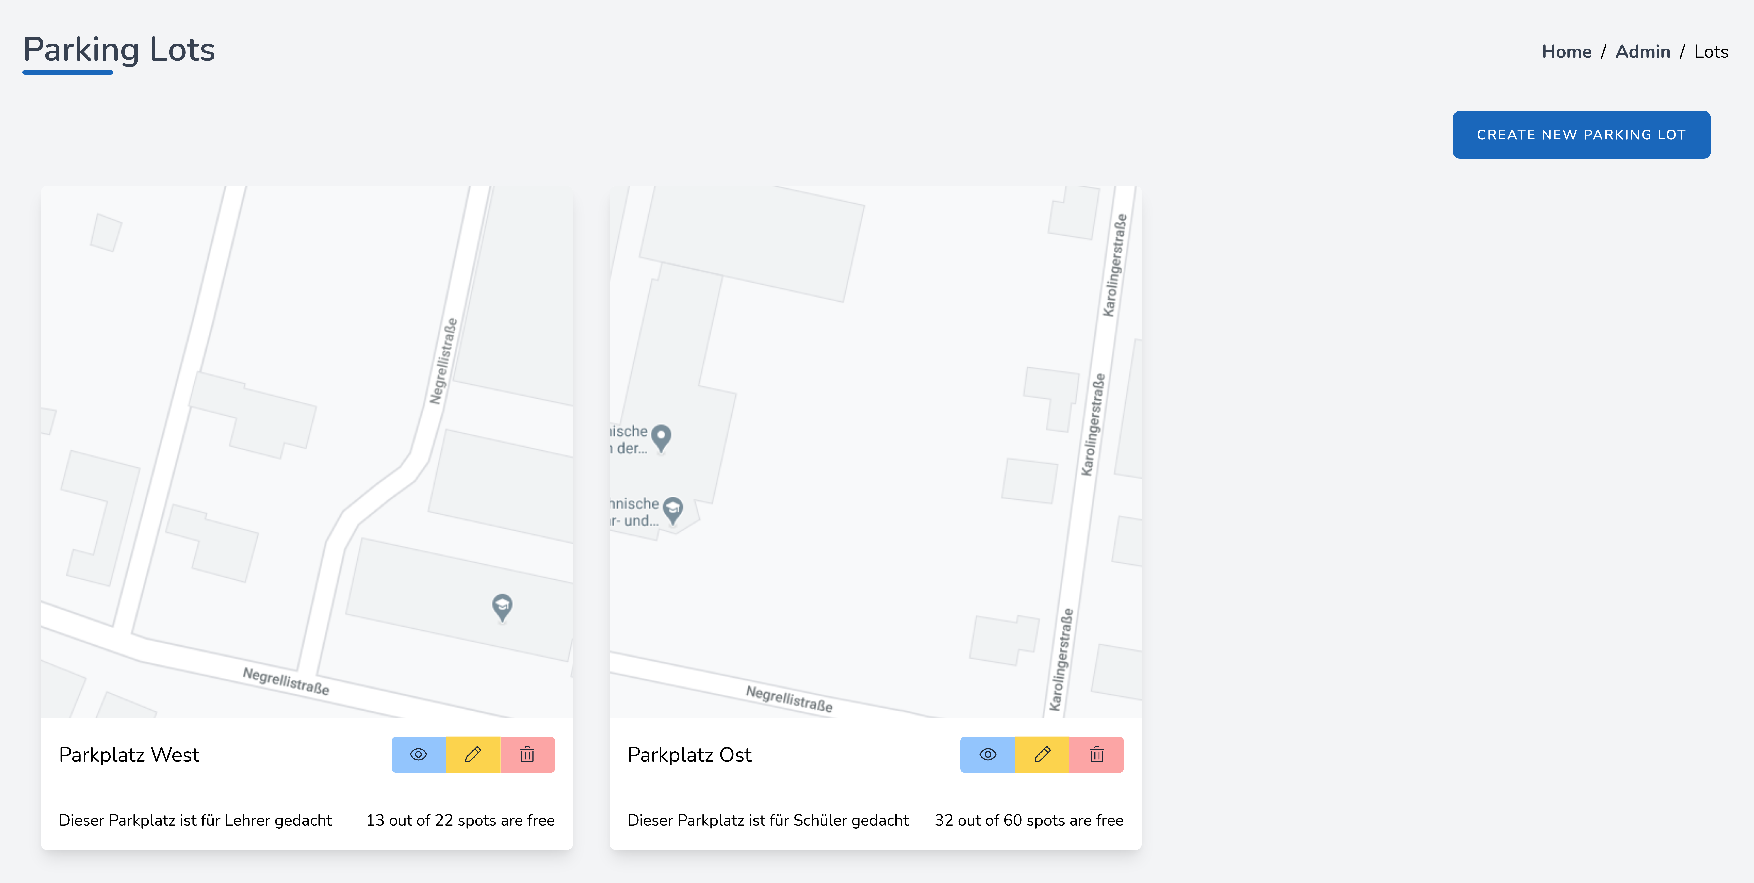
\includegraphics[width=1\linewidth]{webinterface/parking_lots.pdf}}
  \caption{Übersicht aller Parkplätze}
\end{figure}

\paragraph{Parklücken}\mbox{}\\
Eine Parklücke besteht aus einer Adresse und dem Status. Die Adresse ist eine
von der Hardware gesetzte Zahl um die einzelnen Parklücken mit der API zu
identifizieren und anzusteuern. Der Status ist dafür da um anzuzeigen ob eine Parklücke besetzt
oder frei ist.

\begin{figure}[H]
  \centering
  \frame{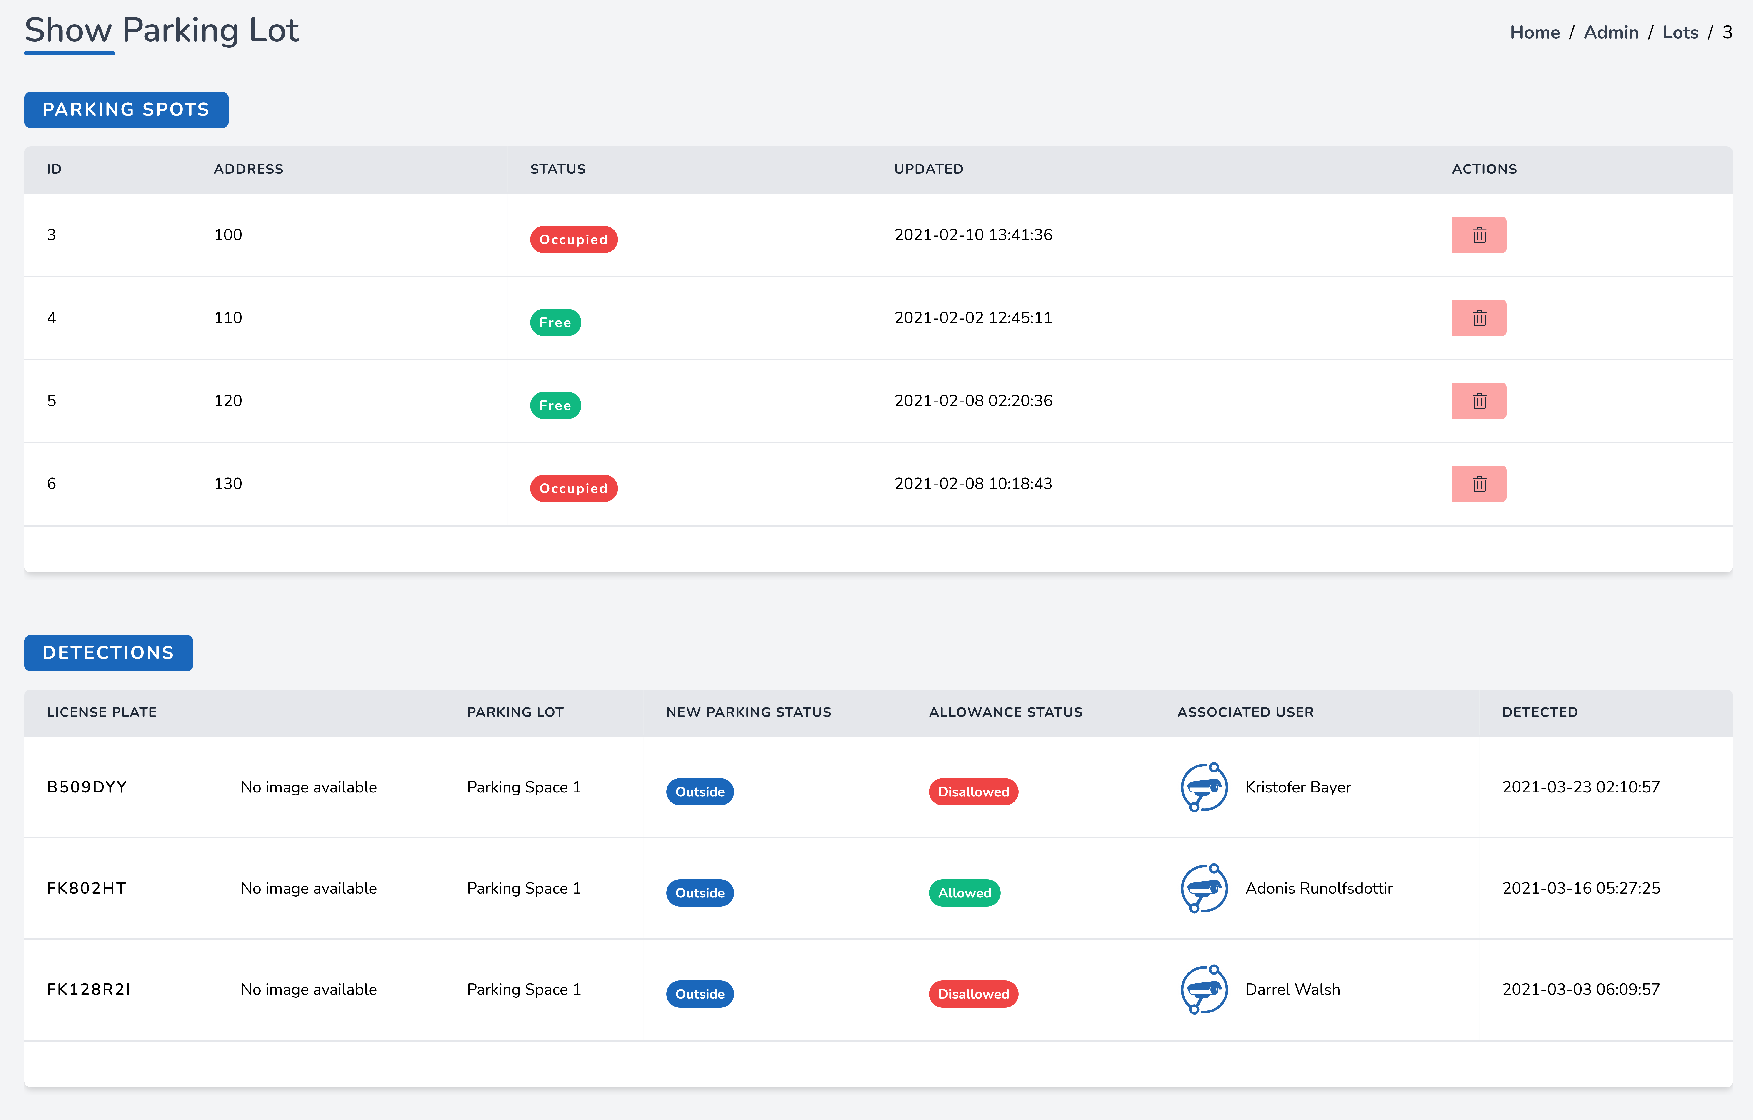
\includegraphics[width=1\linewidth]{webinterface/parking_lot_show.pdf}}
  \caption{Parklücken und Erkennungen eines Parkplatzes}
\end{figure}

%\subsubsection{Kennzeichenverwaltung}
%\subsubsection{Erkennungsverlauf}
\subsubsection{Seiten Einstellungen}
In den Seiten Einstellungen ist es möglich als Benutzer bestimmte Aspekte des
Webinterfaces zu konfigurieren dazu zählt:

\begin{itemize}
  \item Seiten Titel (\verb|key: site_title|)
  \item Standardsprache (\verb|key: default_language|)
  \item Seiten Logo
  \item Erlauben, dass sich neue Benutzer registrieren (\verb|key: allow_new_users|)
  \item Footer Einstellungen (\verb|key: footer_content|)
  \item Inhalt der Datenschutzbestimmungsseite (\verb|key: privacy_policy|)
  \item Inhalt der Allgemeinen Geschäftsbedingungen (\verb|key: terms_of_service|)
  \item Inhalt des Impressums (\verb|key: imprint|)
\end{itemize}

\paragraph{Funktion der Einstellungen}\mbox{}\\

\begin{figure}[H]
  \centering
  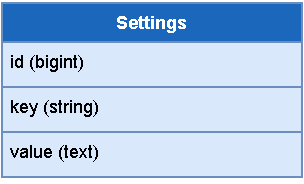
\includegraphics[width=0.35\linewidth]{webinterface/settings_er.pdf}
  \caption{Einstellunge Tabelle}
\end{figure}

Die Einstellungen werden in der Datenbank gespeichert, in der Datenbank besteht eine Einstellung
aus einem \verb|key| und einer \verb|value|. \verb|key| ist dabei vorgegeben und
die \verb|value| kann frei durch das GUI konfiguriert werden.\\

Damit der Browser des Benutzers über die aktuellen Einstellungen bescheid weiß
wird mithilfe eines Service Providers die in der Datenbank vorhandenen
Einstellungen in die Laravel Konfiguration übernommen.

\begin{listing}[H]
  \begin{minted}{php}
    <?php
    public function boot()
    {
      if (Schema::hasTable('settings')) {
        config()->set('settings', \App\Models\Setting::pluck('value', 'key')->all());
      }
    }
  \end{minted}
  \caption{SettingsServiceProvider}
\end{listing}

Nun ist es möglich im Projekt überall mit der \verb|config()| Helper Methode die
Seiten Einstellungen abzurufen. Somit ist es beispielsweise möglich den Seiten
Titel des Webinterfaces in den Layouts anzugeben.

\begin{listing}[H]
  \begin{minted}{html}
    <title>{{ config('settings.site_title') }}</title>
  \end{minted}
  \caption{Seiten Titel Konfiguration}
\end{listing}

\subsubsection{Profil}\label{sec:profile}
Das Profil ist dazu, da um seine eigenen Benutzerinformationen zu betrachten und
zu bearbeiten. Es sind die gleichen Einstellungen wie in der Benutzerverwaltung
einstellbar, jedoch nur über seinen eigenen Account. Eine zusätzliche
Einstellung stellt die UI-Sprache dar, dort kann jeder Benutzer seine gewünschte
UI-Sprache konfigurieren.\\

\begin{figure}[H]
  \centering
  \frame{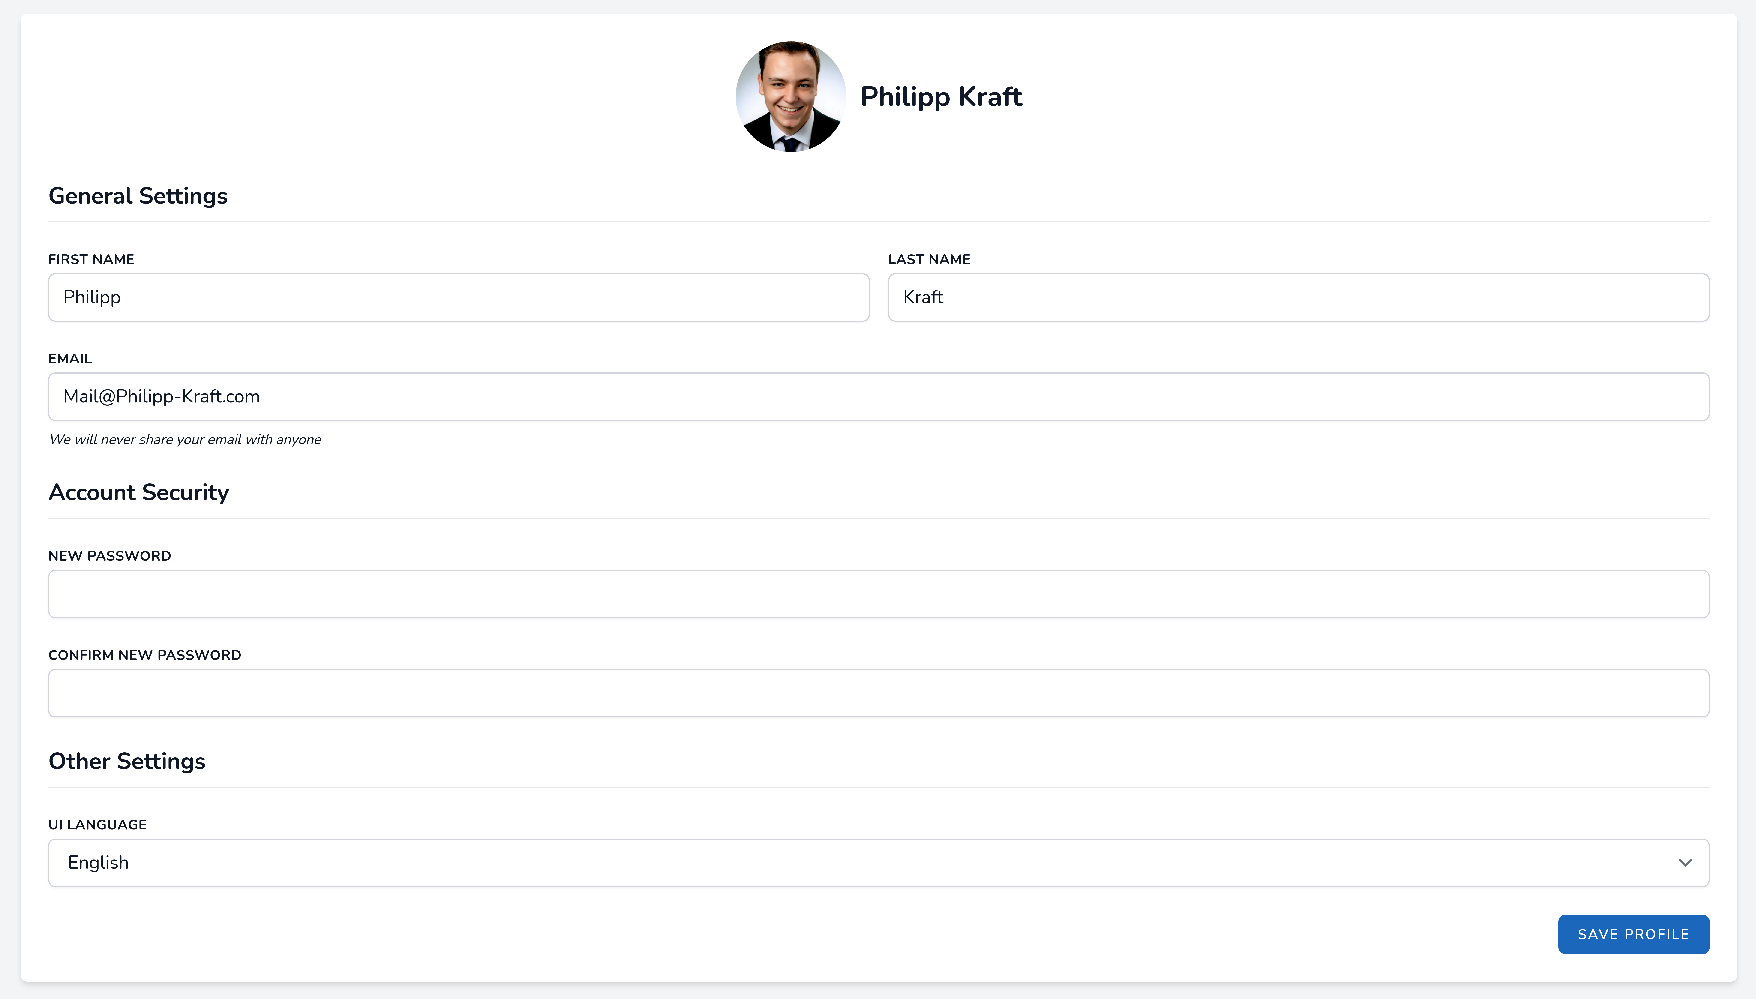
\includegraphics[width=1\linewidth]{webinterface/profile_settings.pdf}}
  \caption{Profil}
\end{figure}

Erreichbar ist das Profil über die Navigationsleiste oben rechts mit einem Klick
auf das Profilbild, es öffnet sich ein Dropdown Menü mit dem Eintrag Profil. 

\begin{figure}[H]
  \centering
  \frame{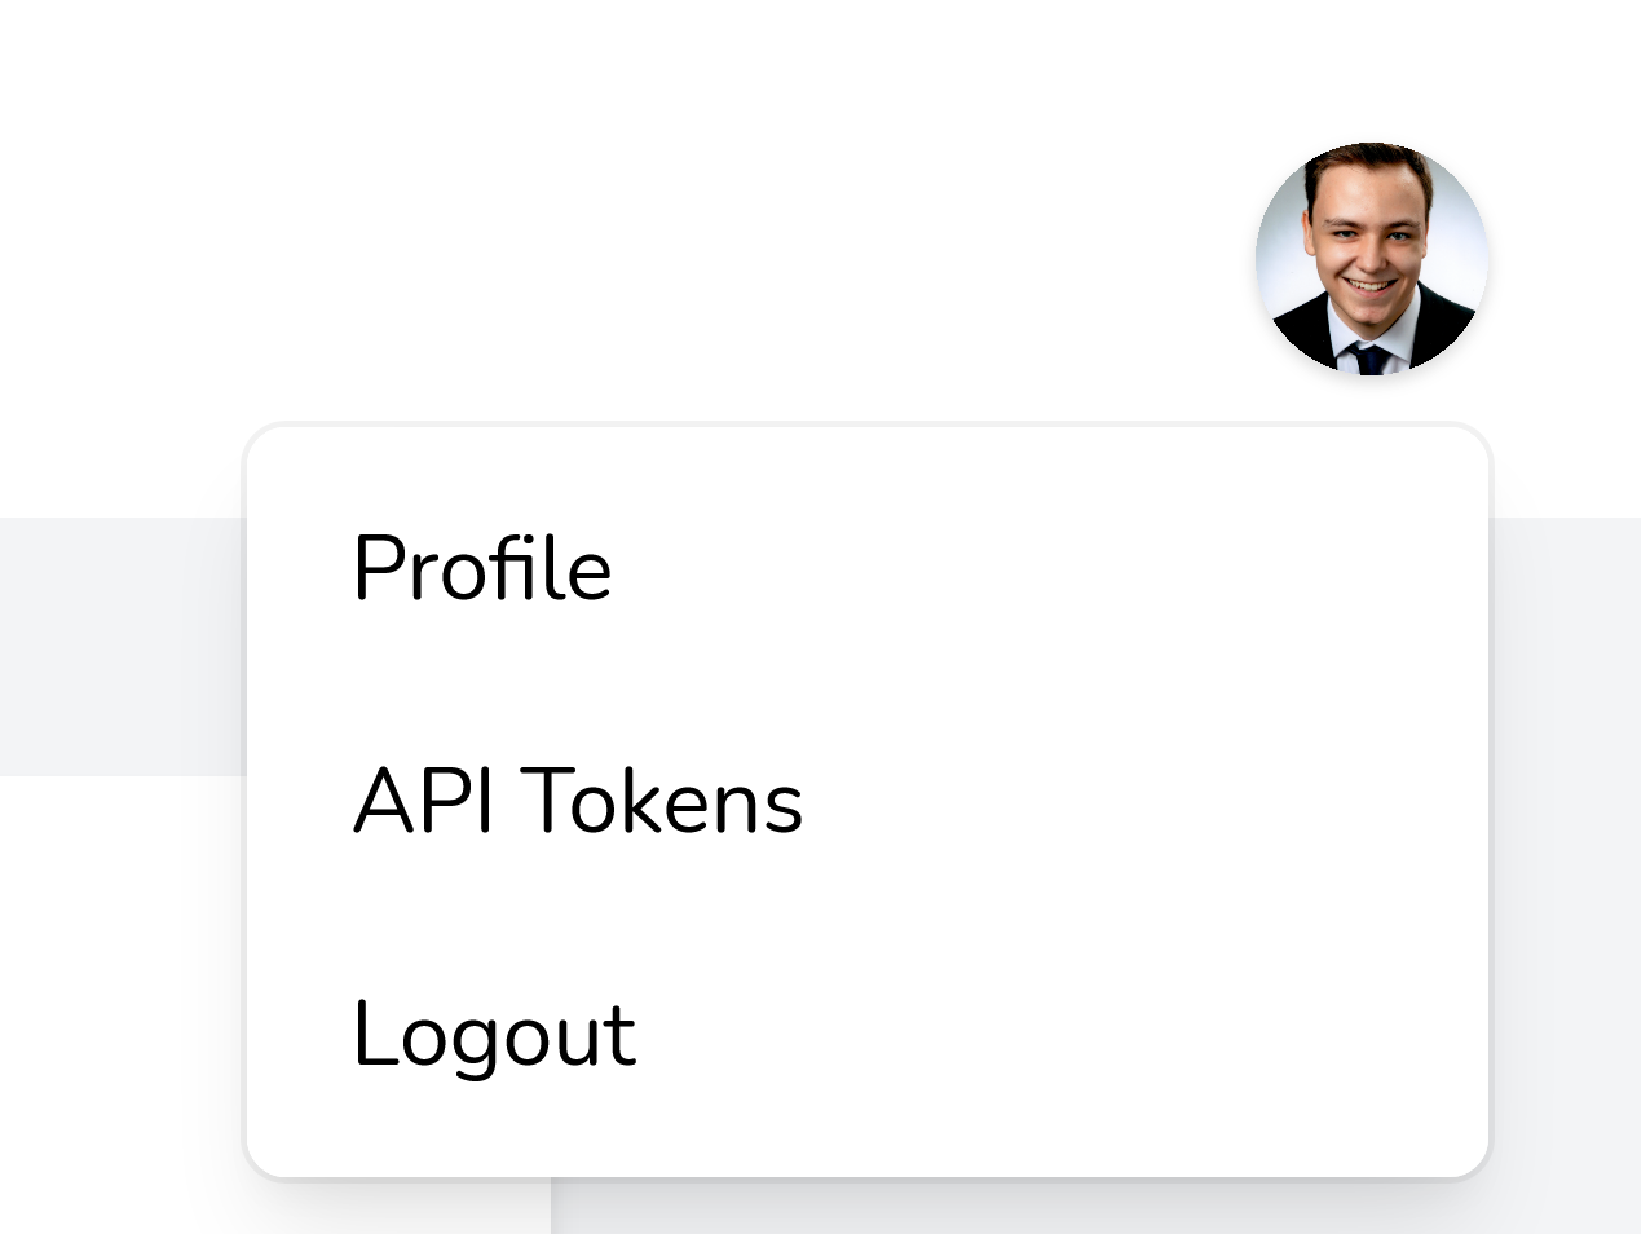
\includegraphics[width=0.4\linewidth]{webinterface/navbar_dropdown.pdf}}
  \caption{Navigationsleiste Dropdown}
\end{figure}

\subsubsection{Lokalisierung}
Lokalisierung ist sehr ähnlich zur Übersetzung, aber anstatt einer wörtlichen
Übersetzung wird die Sprache and das Zielpublikum angepasst. Gegenbenfalls
werden auch Maßeinheiten, Datums- und Uhrzeitformate angepasst.\\

Das Webinterface besitzt die Möglichkeit zwischen Deutsch und Englisch
auszuwählen, hierbei wurde das Webinterface zuerst in Englisch verfasst und dann
in das Deutsche lokalisiert.

\paragraph{Funktion der Sprachauswahl}\mbox{}\\
Wie bereits in der Sektion~\ref{sec:profile} erklärt kann ein Benutzer in den
Profileinstellungen sich eine Sprache je nach Bedürfnis auswählen, dabei wird
diese Sprache nur lokal bei diesem Benutzer angepasst.\\

Bei der Sprachauswahl wird ein \verb|select| Element verwendet, wenn ein
Benutzer nun eine andere Option auswählt wird dieser weitergeleitet,
beispielsweise bei einem Klick auf English wird dieser auf \verb|/locale/en|
weitergeleitet. 

\begin{listing}[H]
  \begin{minted}{php}
    <?php
    <select name="language" onChange="location = this.value;">
    <option {{ Session::get('locale') == 'en' ? 'selected' : '' }}
      value="{{ route('locale', ['locale' => 'en']) }}">
      English</option>
    <option {{ Session::get('locale') == 'de' ? 'selected' : '' }}
      value="{{ route('locale', ['locale' => 'de']) }}">
      Deutsch</option>
    </select>
  \end{minted}
  \caption{Spracheauswahl}
\end{listing}

Beim Aufruf dieser Route wird in die Session des Benutzers die gewünschte
Sprache geschrieben und der Benutzer wird direkt wieder zu der Ursprungsseite
zurück geschickt. Diese Vorgang geht so schnell, dass ein Benutzer nicht
bemerkt, dass die Seite gewechselt wurde.

\begin{listing}[H]
  \begin{minted}{php}
    <?php
    Route::get('locale/{locale}', function ($locale) {
        Session::put('locale', $locale);
        return redirect()->back();
    })->name('locale');
  \end{minted}
  \caption{Spracheauswahl Route}
\end{listing}

Nun steht in der Session des Benutzers die gewünschte Sprache, diese muss nun
angewandt werden. Für das Anwenden der Sprache wird eine \verb|Middleware|
verwendet. Die \verb|Localization| Middleware wird bei jedem Aufruf einer Route
ausgeführt, dabei wird geprüft ob der Benutzer den Eintrag \verb|locale|
besitz, welcher vorhin durch den Service Provider gesetzt wurde und dann wird
die gewünschte Sprache gesetzt.

\begin{listing}[H]
  \begin{minted}{php}
    <?php
    if (\Session::has('locale')) {
      \App::setlocale(\Session::get('locale'));
    } else {
      \App::setlocale(config('settings.default_language'));
      \Session::put('locale', config('settings.default_language'));
    }
  \end{minted}
  \caption{Localization Middleware}
\end{listing}

Besitzt der Benutzer keine \verb|locale| Variable in seiner Session bedeutet,
dass dieser noch keine Sprache festgelegt hat, somit wird automatisch die
ausgewählte Standardsprache aus den Seiten Einstellungen ausgewählt.

\subsection{API}
\subsubsection{Einleitung}
\ac*{API} ist der Teil des Webinterfaces der mit der Hardware kommuniziert.
Diese Programmierschnittstelle ist sehr einfach zu verwenden und wird mit
Laravel Sanctum abgesichert. Die API ermöglicht ein bearbeiten von lesen von
Daten aus dem Webinterface mithilfe von HTTP-Anfragen.

\subsubsection{Autorisierung mit Bearer Token}
Wie bereits besprochen erfolgt die Autorisierung der HTTP-Anfragen mit Laravel
Sanctum. Sanctum verwendet dabei einen sogenannten Bearer Token. Dieser Bearer
Token wird bei Anfragen einfach in der Anfrage im HTTP-Header mitgeschickt und
der Server gleicht dies mit den verschlüsselten Token in der Datenbank ab
erlaubt oder verweigert den Zugriff.

\subsubsection{API Tokens erstellen}
Über das Webinterface kann entweder über die Sidebar oder über das Dropdown Menü
in der Navigationsleiste das Menü \textit{API Tokens} erreicht werden. Dort
können nun neue API Tokens erstellt werden, zur späteren Identifikation kann
diesem API Token mit einem Namen versehen werden, dieser Name spielt aber
ansonsten keine Rolle. 

\begin{figure}[H]
  \centering
  \frame{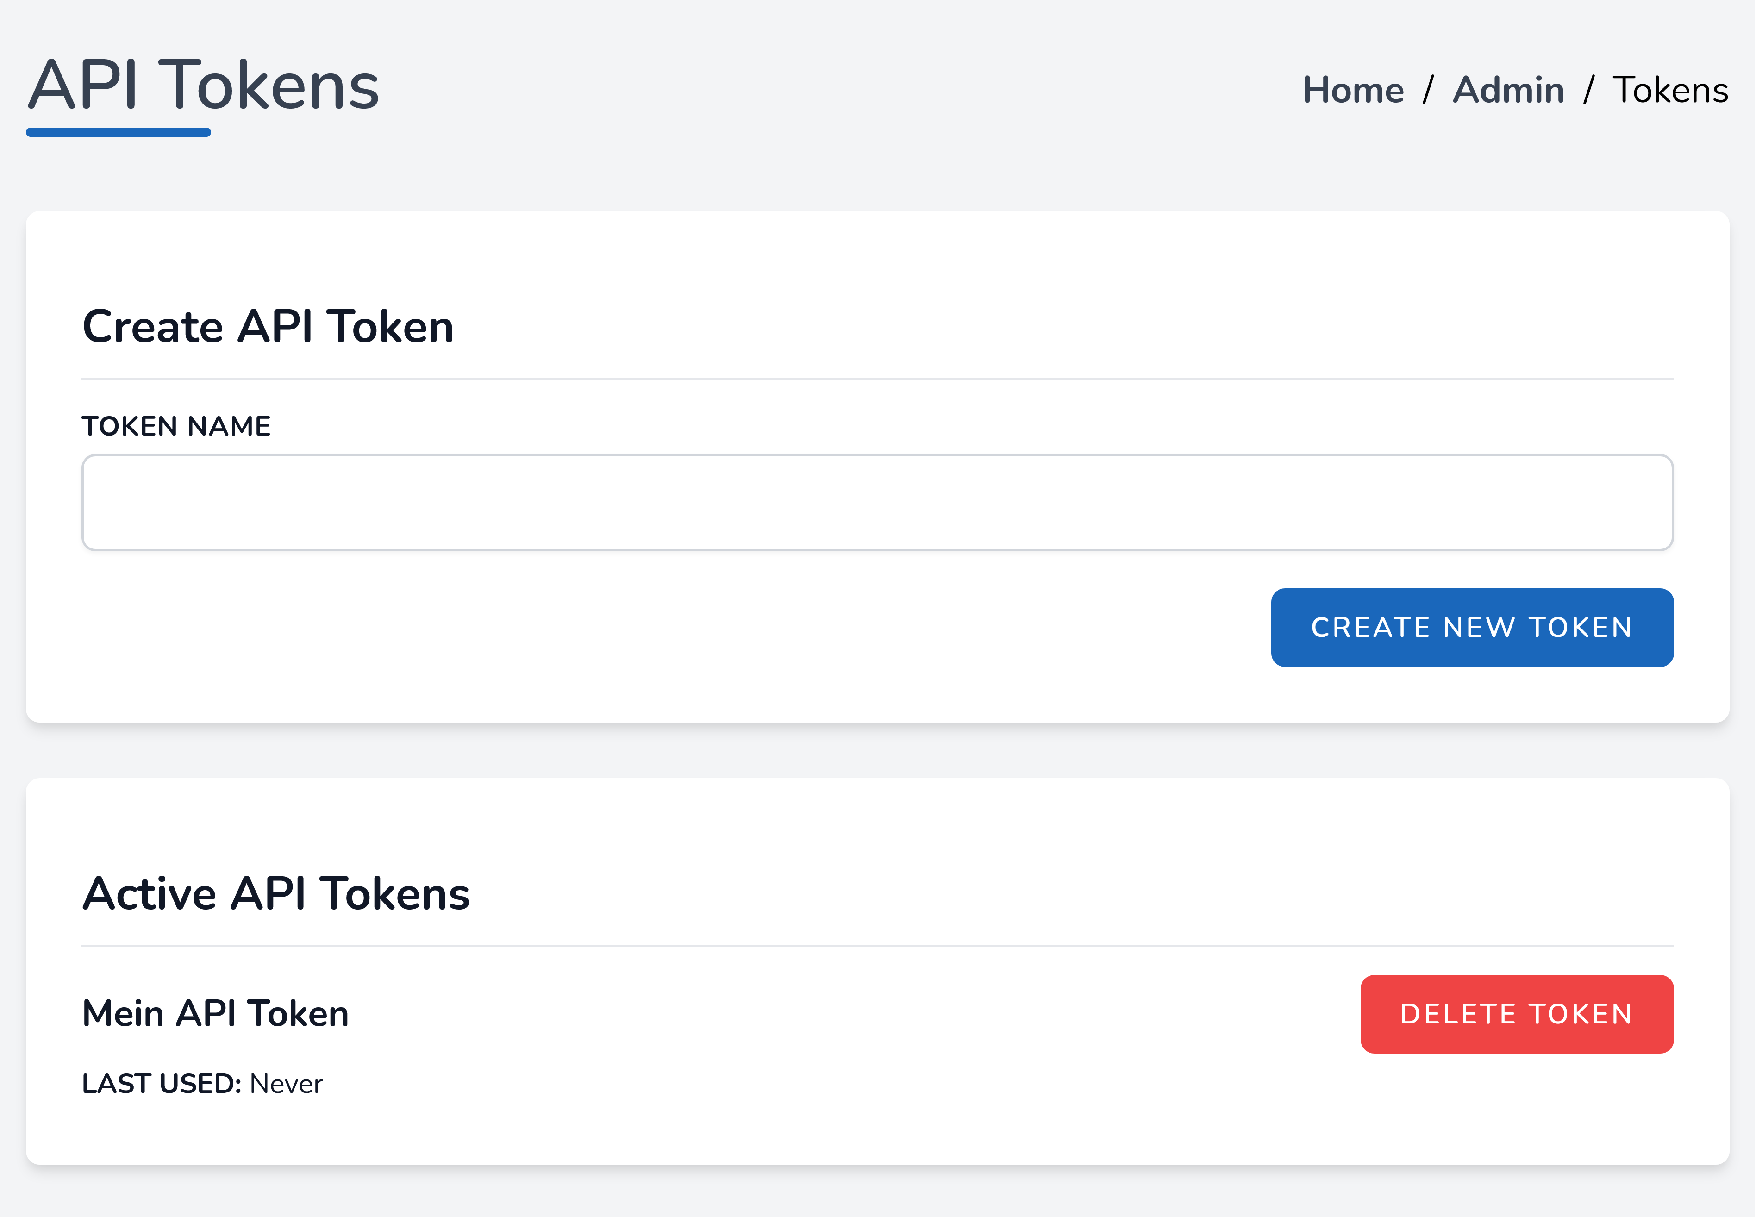
\includegraphics[width=1\linewidth]{webinterface/create_api_token.pdf}}
  \caption{API Token}
\end{figure}

Beim erstellen des API Tokens öffnet sich einmalig ein Popup mit dem Bearer
Token, dieser muss nun abgespeichert werden, denn der Token wird aus
Sicherheitsgründen nur einmalig angezeigt.

\begin{figure}[H]
  \centering
  \frame{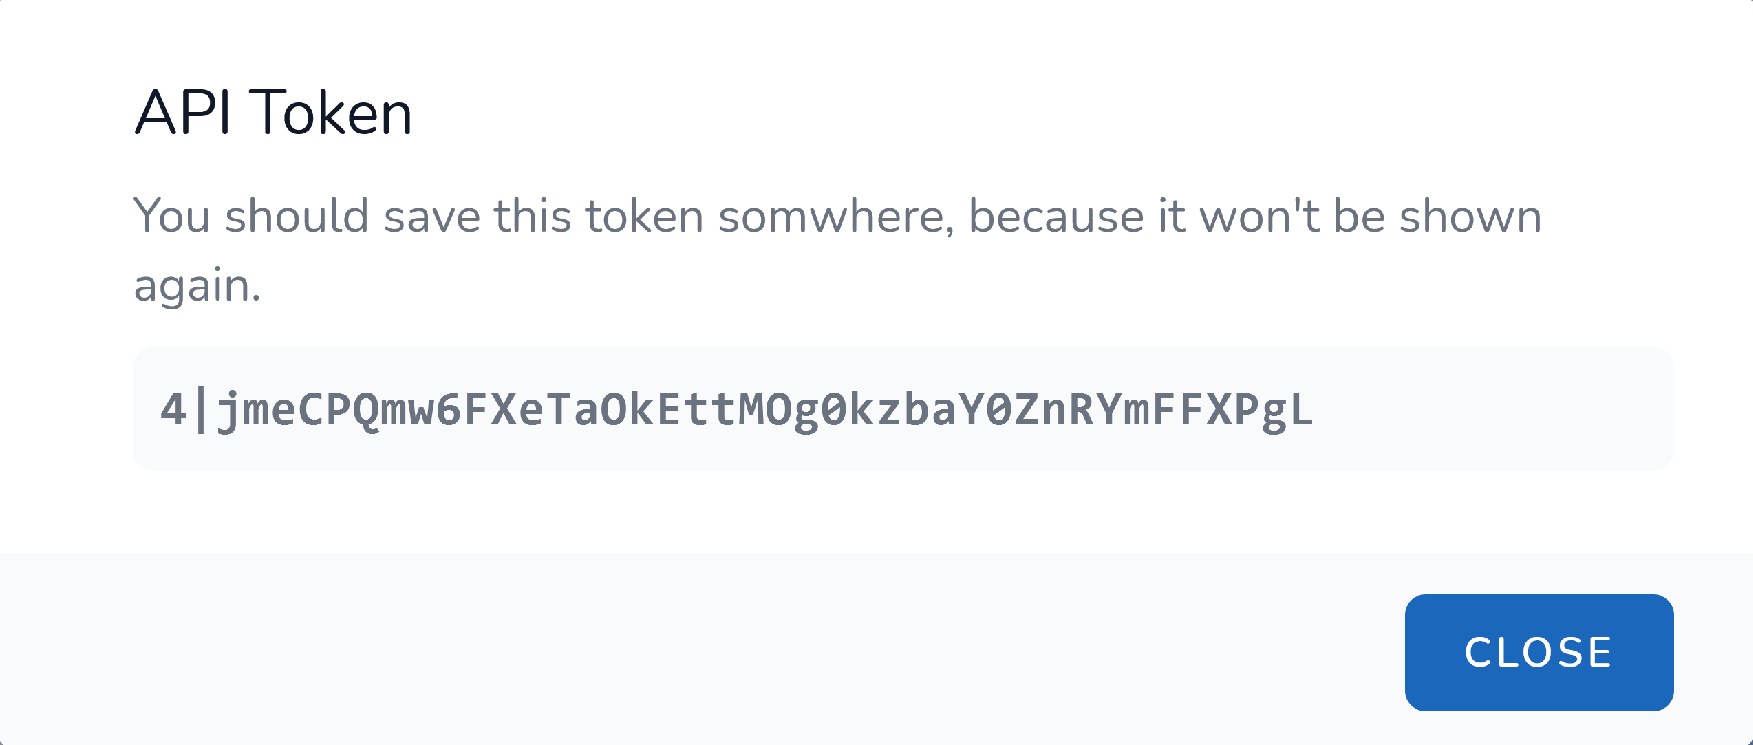
\includegraphics[width=0.5\linewidth]{webinterface/api_token.pdf}}
  \caption{API Token Popup}
\end{figure}

\subsubsection{Erkennungen}
\paragraph{GET /api/v1/detections}\mbox{}\\

\begin{table}[H]
  \centering
  \begin{tabular}{|l|l|}
  \hline
  \multicolumn{2}{|c|}{\textbf{Erkennungen GET}} \\ \hline
  \textbf{Pfad}                & /api/v1/detections  \\ \hline
  \textbf{Beschreibung}        &                     \\ \hline
  \textbf{HTTP-Methode}        & GET                 \\ \hline
  \textbf{Authentifizierung}   & Bearer Token        \\ \hline
  \textbf{Rückgabetyp}         & application/json    \\ \hline
  \multicolumn{2}{|c|}{\textbf{Path Parameter}}                      \\ \hline
  \multicolumn{2}{|c|}{None}          \\ \hline
  \multicolumn{2}{|c|}{\textbf{Query Parameter}}                      \\ \hline
  \multicolumn{2}{|c|}{None}          \\ \hline
  \end{tabular}
  \caption{GET /api/v1/detections}
\end{table}

Die Rückgabe entspricht der Rückgabe von \verb|GET /api/v1/detections/{id}|, jedoch wird ein
Array von Erkennungen geliefert.

\paragraph{GET /api/v1/detections/\{id\}}\mbox{}\\

\begin{table}[H]
  \centering
  \begin{tabular}{|l|l|}
  \hline
  \multicolumn{2}{|c|}{\textbf{Erkennungen GET}}         \\ \hline
  \textbf{Pfad}              & /api/v1/detections        \\ \hline
  \textbf{Beschreibung}      &                           \\ \hline
  \textbf{HTTP-Methode}      & GET                       \\ \hline
  \textbf{Authentifizierung} & Bearer Token              \\ \hline
  \textbf{Rückgabetyp}       & application/json          \\ \hline
  \multicolumn{2}{|c|}{\textbf{Path Parameter}}          \\ \hline
  id                         & Required: true            \\ \hline
                             & Type: int                 \\ \hline
                             & Description: Detection Id \\ \hline
  \multicolumn{2}{|c|}{\textbf{Query Parameter}}                      \\ \hline
  \multicolumn{2}{|c|}{None}          \\ \hline
  \end{tabular}
  \caption{GET /api/v1/detections/\{id\}}
\end{table}

\begin{listing}[H]
  \begin{minted}{js}
    {
        "id": 1,
        "license_plate_id": 69,
        "parking_lot_id": 3,
        "parking_status": "Outside",
        "image": null,
        "created_at": "2021-03-23T02:10:57.000000Z",
        "updated_at": "2021-03-09T02:08:54.000000Z",
        "license_plate": {
            "id": 69,
            "user_id": 74,
            "name": "B509DYY",
            "country": "Austria",
            "parking_status": "Outside",
            "allowance_status": "Disallowed",
            "created_at": "2020-11-19T17:26:03.000000Z",
            "updated_at": "2021-03-20T21:12:24.000000Z"
        },
        "parking_lot": {
            "id": 3,
            "name": "Parking Space 1",
            "description": null,
            "image": "default.png",
            "created_at": "2021-03-31T22:40:24.000000Z",
            "updated_at": "2021-03-31T22:42:57.000000Z"
        }
    }
  \end{minted}
  \caption{Beispielhafte GET /api/v1/detections/\{id\} Rückgabe}
\end{listing}

\paragraph{POST /api/v1/detections}\mbox{}\\

\begin{table}[H]
  \centering
  \begin{tabular}{|l|l|}
  \hline
  \multicolumn{2}{|c|}{\textbf{Erkennungen POST}}          \\ \hline
  \textbf{Pfad}              & /api/v1/detections              \\ \hline
  \textbf{Beschreibung}      &                                 \\ \hline
  \textbf{HTTP-Methode}      & POST                            \\ \hline
  \textbf{Authentifizierung} & Bearer Token                    \\ \hline
  \textbf{Rückgabetyp}       & application/json                \\ \hline
  \multicolumn{2}{|c|}{\textbf{Query Parameter}}               \\ \hline
  name                       & Required: true                  \\ \hline
                             & Type: string                    \\ \hline
                             & Description: License plate name \\ \hline
  parking\_lot\_id           & Required: true                  \\ \hline
                             & Type: int                       \\ \hline
                             & Description: Parking Lot Id     \\ \hline
  \multicolumn{2}{|c|}{\textbf{Query Parameter}}                      \\ \hline
  \multicolumn{2}{|c|}{None}          \\ \hline
  \end{tabular}
  \caption{POST /api/v1/detections}
\end{table}

Die Rückgabe entspricht der Rückgabe von \verb|GET /api/v1/detections/{id}|.

\subsubsection{Kennzeichen}
\paragraph{GET /api/v1/plates}\mbox{}\\

\begin{table}[H]
  \centering
  \begin{tabular}{|l|l|}
  \hline
  \multicolumn{2}{|c|}{\textbf{Kennzeichen GET}} \\ \hline
  \textbf{Pfad}                & /api/v1/plates  \\ \hline
  \textbf{Beschreibung}        &                     \\ \hline
  \textbf{HTTP-Methode}        & GET                 \\ \hline
  \textbf{Authentifizierung}   & Bearer Token        \\ \hline
  \textbf{Rückgabetyp}         & application/json    \\ \hline
  \multicolumn{2}{|c|}{\textbf{Path Parameter}}                      \\ \hline
  \multicolumn{2}{|c|}{None}          \\ \hline
  \multicolumn{2}{|c|}{\textbf{Query Parameter}}                      \\ \hline
  \multicolumn{2}{|c|}{None}          \\ \hline
  \end{tabular}
  \caption{GET /api/v1/plates}
\end{table}

Die Rückgabe entspricht \verb|GET /api/v1/plates/{id}|, jedoch wird ein
Array mit einzelnen Kennzeichen geliefert.

\paragraph{GET /api/v1/plates/\{id\}}\mbox{}\\

\begin{table}[H]
  \centering
  \begin{tabular}{|l|l|}
  \hline
  \multicolumn{2}{|c|}{\textbf{Kennzeichen GET}}         \\ \hline
  \textbf{Pfad}              & /api/v1/plates        \\ \hline
  \textbf{Beschreibung}      &                           \\ \hline
  \textbf{HTTP-Methode}      & GET                       \\ \hline
  \textbf{Authentifizierung} & Bearer Token              \\ \hline
  \textbf{Rückgabetyp}       & application/json          \\ \hline
  \multicolumn{2}{|c|}{\textbf{Path Parameter}}          \\ \hline
  id                         & Required: true            \\ \hline
                             & Type: int                 \\ \hline
                             & Description: License Plate Id \\ \hline
  \end{tabular}
  \caption{GET /api/v1/plates/\{id\}}
\end{table}

\begin{listing}[H]
  \begin{minted}{js}
    {
        "id": 1,
        "user_id": 8,
        "name": "FK8VD0",
        "country": "Austria",
        "parking_status": "Inside",
        "allowance_status": "Unknown",
        "created_at": "2020-12-05T07:04:31.000000Z",
        "updated_at": "2021-03-22T09:31:46.000000Z",
        "detections": [
            {
                "id": 149,
                "license_plate_id": 1,
                "parking_lot_id": 2,
                "parking_status": "Inside",
                "image": null,
                "created_at": "2021-03-12T18:18:40.000000Z",
                "updated_at": "2021-03-22T11:46:44.000000Z"
            },
            ...
        ]
    }
  \end{minted}
  \caption{Beispielhafte GET /api/v1/plates/\{id\} Rückgabe}
\end{listing}

\subsubsection{Parkplätze}
\paragraph{GET /api/v1/lots}\mbox{}\\

\begin{table}[H]
  \centering
  \begin{tabular}{|l|l|}
  \hline
  \multicolumn{2}{|c|}{\textbf{Parkplätze GET}} \\ \hline
  \textbf{Pfad}                & /api/v1/lots  \\ \hline
  \textbf{Beschreibung}        &                     \\ \hline
  \textbf{HTTP-Methode}        & GET                 \\ \hline
  \textbf{Authentifizierung}   & Bearer Token        \\ \hline
  \textbf{Rückgabetyp}         & application/json    \\ \hline
  \multicolumn{2}{|c|}{\textbf{Path Parameter}}                      \\ \hline
  \multicolumn{2}{|c|}{None}          \\ \hline
  \multicolumn{2}{|c|}{\textbf{Query Parameter}}                      \\ \hline
  \multicolumn{2}{|c|}{None}          \\ \hline
  \end{tabular}
  \caption{GET /api/v1/lots}
\end{table}

Die Rückgabe entspricht \verb|GET /api/v1/lots/{i\}|, jedoch wird ein
Array von einzelnen Parkplätzen geliefert.

\paragraph{GET /api/v1/lots/\{id\}}\mbox{}\\

\begin{table}[H]
  \centering
  \begin{tabular}{|l|l|}
  \hline
  \multicolumn{2}{|c|}{\textbf{Parkplätze GET}}         \\ \hline
  \textbf{Pfad}              & /api/v1/lots        \\ \hline
  \textbf{Beschreibung}      &                           \\ \hline
  \textbf{HTTP-Methode}      & GET                       \\ \hline
  \textbf{Authentifizierung} & Bearer Token              \\ \hline
  \textbf{Rückgabetyp}       & application/json          \\ \hline
  \multicolumn{2}{|c|}{\textbf{Path Parameter}}          \\ \hline
  id                         & Required: true            \\ \hline
                             & Type: int                 \\ \hline
                             & Description: Parking Lot Id \\ \hline
  \multicolumn{2}{|c|}{\textbf{Query Parameter}}                      \\ \hline
  \multicolumn{2}{|c|}{None}          \\ \hline
  \end{tabular}
  \caption{GET /api/v1/lots/\{id\}}
\end{table}

\begin{listing}[H]
  \begin{minted}{js}
    {
        "id": 3,
        "name": "Parking Space 1",
        "description": null,
        "image": "default.png",
        "created_at": "2021-03-31T22:40:24.000000Z",
        "updated_at": "2021-03-31T22:42:57.000000Z",
        "detections": [
            {
                "id": 1,
                "license_plate_id": 69,
                "parking_lot_id": 3,
                "parking_status": "Outside",
                "image": null,
                "created_at": "2021-03-23T02:10:57.000000Z",
                "updated_at": "2021-03-09T02:08:54.000000Z"
            },
            ...
        ]
    }
  \end{minted}
  \caption{Beispielhafte GET /api/v1/lots/\{id\} Rückgabe}
\end{listing}

\subsubsection{Parklücken}
\paragraph{GET /api/v1/spots}\mbox{}\\

\begin{table}[H]
  \centering
  \begin{tabular}{|l|l|}
  \hline
  \multicolumn{2}{|c|}{\textbf{Parklücke GET}} \\ \hline
  \textbf{Pfad}                & /api/v1/spots  \\ \hline
  \textbf{Beschreibung}        &                     \\ \hline
  \textbf{HTTP-Methode}        & GET                 \\ \hline
  \textbf{Authentifizierung}   & Bearer Token        \\ \hline
  \textbf{Rückgabetyp}         & application/json    \\ \hline
  \multicolumn{2}{|c|}{\textbf{Path Parameter}}                      \\ \hline
  \multicolumn{2}{|c|}{None}          \\ \hline
  \multicolumn{2}{|c|}{\textbf{Query Parameter}}                      \\ \hline
  \multicolumn{2}{|c|}{None}          \\ \hline
  \end{tabular}
  \caption{GET /api/v1/spots}
\end{table}

Die Rückgabe entspricht \verb|GET /api/v1/spots/{id}|, jedoch wird ein
Array von einzelnen Parklücken geliefert.

\paragraph{GET /api/v1/spots/\{id\}}\mbox{}\\

\begin{table}[H]
  \centering
  \begin{tabular}{|l|l|}
  \hline
  \multicolumn{2}{|c|}{\textbf{Parklücke GET}}         \\ \hline
  \textbf{Pfad}              & /api/v1/spots        \\ \hline
  \textbf{Beschreibung}      &                           \\ \hline
  \textbf{HTTP-Methode}      & GET                       \\ \hline
  \textbf{Authentifizierung} & Bearer Token              \\ \hline
  \textbf{Rückgabetyp}       & application/json          \\ \hline
  \multicolumn{2}{|c|}{\textbf{Path Parameter}}          \\ \hline
  id                         & Required: true            \\ \hline
                             & Type: int                 \\ \hline
                             & Description: Parking Spot Id \\ \hline
  \multicolumn{2}{|c|}{\textbf{Query Parameter}}                      \\ \hline
  \multicolumn{2}{|c|}{None}          \\ \hline
  \end{tabular}
  \caption{GET /api/v1/spots/\{id\}}
\end{table}

\begin{listing}[H]
  \begin{minted}{js}
    {
        "id": 40,
        "address": null,
        "parking_lot_id": 2,
        "occupied": 0,
        "created_at": "2021-03-22T17:51:10.000000Z",
        "updated_at": "2021-02-13T23:23:55.000000Z",
        "parking_lot": {
            "id": 2,
            "name": "Parkplatz Ost",
            "description": "Dieser Parkplatz ist für Schüler gedacht",
            "image": "parkplatz_ost.png",
            "created_at": "2021-03-30T15:44:19.000000Z",
            "updated_at": "2021-03-30T15:44:19.000000Z"
        }
    }
  \end{minted}
  \caption{Beispielhafte GET /api/v1/spots/\{id\} Rückgabe}
\end{listing}

\paragraph{POST /api/v1/lots/\{id\}/spots}\mbox{}\\

\begin{table}[H]
  \centering
  \begin{tabular}{|l|l|}
  \hline
  \multicolumn{2}{|c|}{\textbf{Parklücken POST}}                  \\ \hline
  \textbf{Pfad}              & /api/v1/lots/\{id\}/spots              \\ \hline
  \textbf{Beschreibung}      &                                        \\ \hline
  \textbf{HTTP-Methode}      & POST                                   \\ \hline
  \textbf{Authentifizierung} & Bearer Token                           \\ \hline
  \textbf{Rückgabetyp}       & application/json                       \\ \hline
  \multicolumn{2}{|c|}{\textbf{Path Parameter}}                       \\ \hline
  id                         & Required: true                         \\ \hline
                             & Type: int                              \\ \hline
                             & Description: Parking Lot Id            \\ \hline
  \multicolumn{2}{|c|}{\textbf{Query Parameter}}                      \\ \hline
  address                    & Required: true                         \\ \hline
                             & Type: int                              \\ \hline
                             & Description: Hardware Adresse          \\ \hline
  occupied                   & Required: true                         \\ \hline
                             & Type: bool                             \\ \hline
                             & Description: 1 for occupied 0 for free \\ \hline
  \end{tabular}
  \caption{POST /api/v1/lots/\{id\}/spots}
\end{table}

\begin{listing}[H]
  \begin{minted}{js}
    {
      "id": 101,
      "address": 1337,
      "parking_lot_id": 1,
      "occupied": 0,
      "created_at": "2021-03-31T22:27:21.000000Z",
      "updated_at": "2021-03-31T22:27:21.000000Z",
      "parking_lot": {
          "id": 1,
          "name": "Parkplatz West",
          "description": "Dieser Parkplatz ist für Lehrer gedacht",
          "image": "parkplatz_west.png",
          "created_at": "2021-03-30T15:44:19.000000Z",
          "updated_at": "2021-03-30T15:44:19.000000Z"
      }
    }
  \end{minted}
  \caption{Beispielhafte POST /api/v1/lots/\{id\}/spots Rückgabe}
\end{listing}

\subsubsection{Einstellungen}
\paragraph{GET /api/v1/settings}\mbox{}\\

\begin{table}[H]
  \centering
  \begin{tabular}{|l|l|}
  \hline
  \multicolumn{2}{|c|}{\textbf{Einstellungen GET}} \\ \hline
  \textbf{Pfad}                & /api/v1/settings  \\ \hline
  \textbf{Beschreibung}        &                     \\ \hline
  \textbf{HTTP-Methode}        & GET                 \\ \hline
  \textbf{Authentifizierung}   & Bearer Token        \\ \hline
  \textbf{Rückgabetyp}         & application/json    \\ \hline
  \multicolumn{2}{|c|}{\textbf{Path Parameter}}                      \\ \hline
  \multicolumn{2}{|c|}{None}          \\ \hline
  \multicolumn{2}{|c|}{\textbf{Query Parameter}}                      \\ \hline
  \multicolumn{2}{|c|}{None}          \\ \hline
  \end{tabular}
  \caption{GET /api/v1/settings}
\end{table}

\begin{listing}[H]
  \begin{minted}{js}
    [
        {
            "id": 1,
            "key": "site_title",
            "value": "APM"
        },
        ...
    ]
  \end{minted}
  \caption{Beispielhafte GET /api/v1/settings Rückgabe}
\end{listing}

\subsubsection{Benutzer}
\paragraph{GET /api/v1/users}\mbox{}\\

\begin{table}[H]
  \centering
  \begin{tabular}{|l|l|}
  \hline
  \multicolumn{2}{|c|}{\textbf{Benutzer GET}} \\ \hline
  \textbf{Pfad}                & /api/v1/users  \\ \hline
  \textbf{Beschreibung}        &                     \\ \hline
  \textbf{HTTP-Methode}        & GET                 \\ \hline
  \textbf{Authentifizierung}   & Bearer Token        \\ \hline
  \textbf{Rückgabetyp}         & application/json    \\ \hline
  \multicolumn{2}{|c|}{\textbf{Path Parameter}}                      \\ \hline
  \multicolumn{2}{|c|}{None}          \\ \hline
  \multicolumn{2}{|c|}{\textbf{Query Parameter}}                      \\ \hline
  \multicolumn{2}{|c|}{None}          \\ \hline
  \end{tabular}
  \caption{GET /api/v1/users}
\end{table}

Die Rückgabe entspricht \verb|GET /api/v1/users/{id}|, jedoch wird ein
Array von einzelnen Benutzern geliefert.

\paragraph{GET /api/v1/users/\{id\}}\mbox{}\\

\begin{table}[H]
  \centering
  \begin{tabular}{|l|l|}
  \hline
  \multicolumn{2}{|c|}{\textbf{Benutzer GET}}         \\ \hline
  \textbf{Pfad}              & /api/v1/users        \\ \hline
  \textbf{Beschreibung}      &                           \\ \hline
  \textbf{HTTP-Methode}      & GET                       \\ \hline
  \textbf{Authentifizierung} & Bearer Token              \\ \hline
  \textbf{Rückgabetyp}       & application/json          \\ \hline
  \multicolumn{2}{|c|}{\textbf{Path Parameter}}          \\ \hline
  id                         & Required: true            \\ \hline
                             & Type: int                 \\ \hline
                             & Description: User Id \\ \hline
  \multicolumn{2}{|c|}{\textbf{Query Parameter}}                      \\ \hline
  \multicolumn{2}{|c|}{None}          \\ \hline
  \end{tabular}
  \caption{GET /api/v1/users/\{id\}}
\end{table}

\begin{listing}[H]
  \begin{minted}{js}
    {
        "id": 1,
        "first_name": "Philipp",
        "last_name": "Kraft",
        "email": "Mail@Philipp-Kraft.com",
        "avatar": "philipp.png",
        "email_verified_at": "2021-03-30T15:44:18.000000Z",
        "last_login_ip": "127.0.0.1",
        "last_login_at": "2021-04-01 09:22:01",
        "created_at": "2021-03-30T15:44:18.000000Z",
        "updated_at": "2021-04-01T09:22:01.000000Z",
        "license_plates": []
    }
  \end{minted}
  \caption{Beispielhafte GET /api/v1/users/\{id\} Rückgabe}
\end{listing}